\documentclass[10pt]{article}
\usepackage[utf8]{inputenc}
\usepackage[T1]{fontenc}
\usepackage{amsmath}
\usepackage{amsfonts}
\usepackage{amssymb}
\usepackage[version=4]{mhchem}
\usepackage{stmaryrd}
\usepackage{mathrsfs}
\usepackage{graphicx}
\usepackage[export]{adjustbox}
\graphicspath{ {./images/} }
\usepackage{bbold}

\title{Classification }


\author{Machine Learning Course - CS-433\\
Oct 17, 2023\\
Nicolas Flammarion}
\date{}


\begin{document}
\maketitle
EPFL

\section*{Definition of classification}
We observe some data $S=\left\{x_{n}, y_{n}\right\}_{n=1}^{N} \in \mathscr{X} \times \underbrace{\mathscr{Y}}_{\text {Discrete Set }}$

Goal: given a new observation $x$, we want to predict its label $y$

How:

\begin{center}
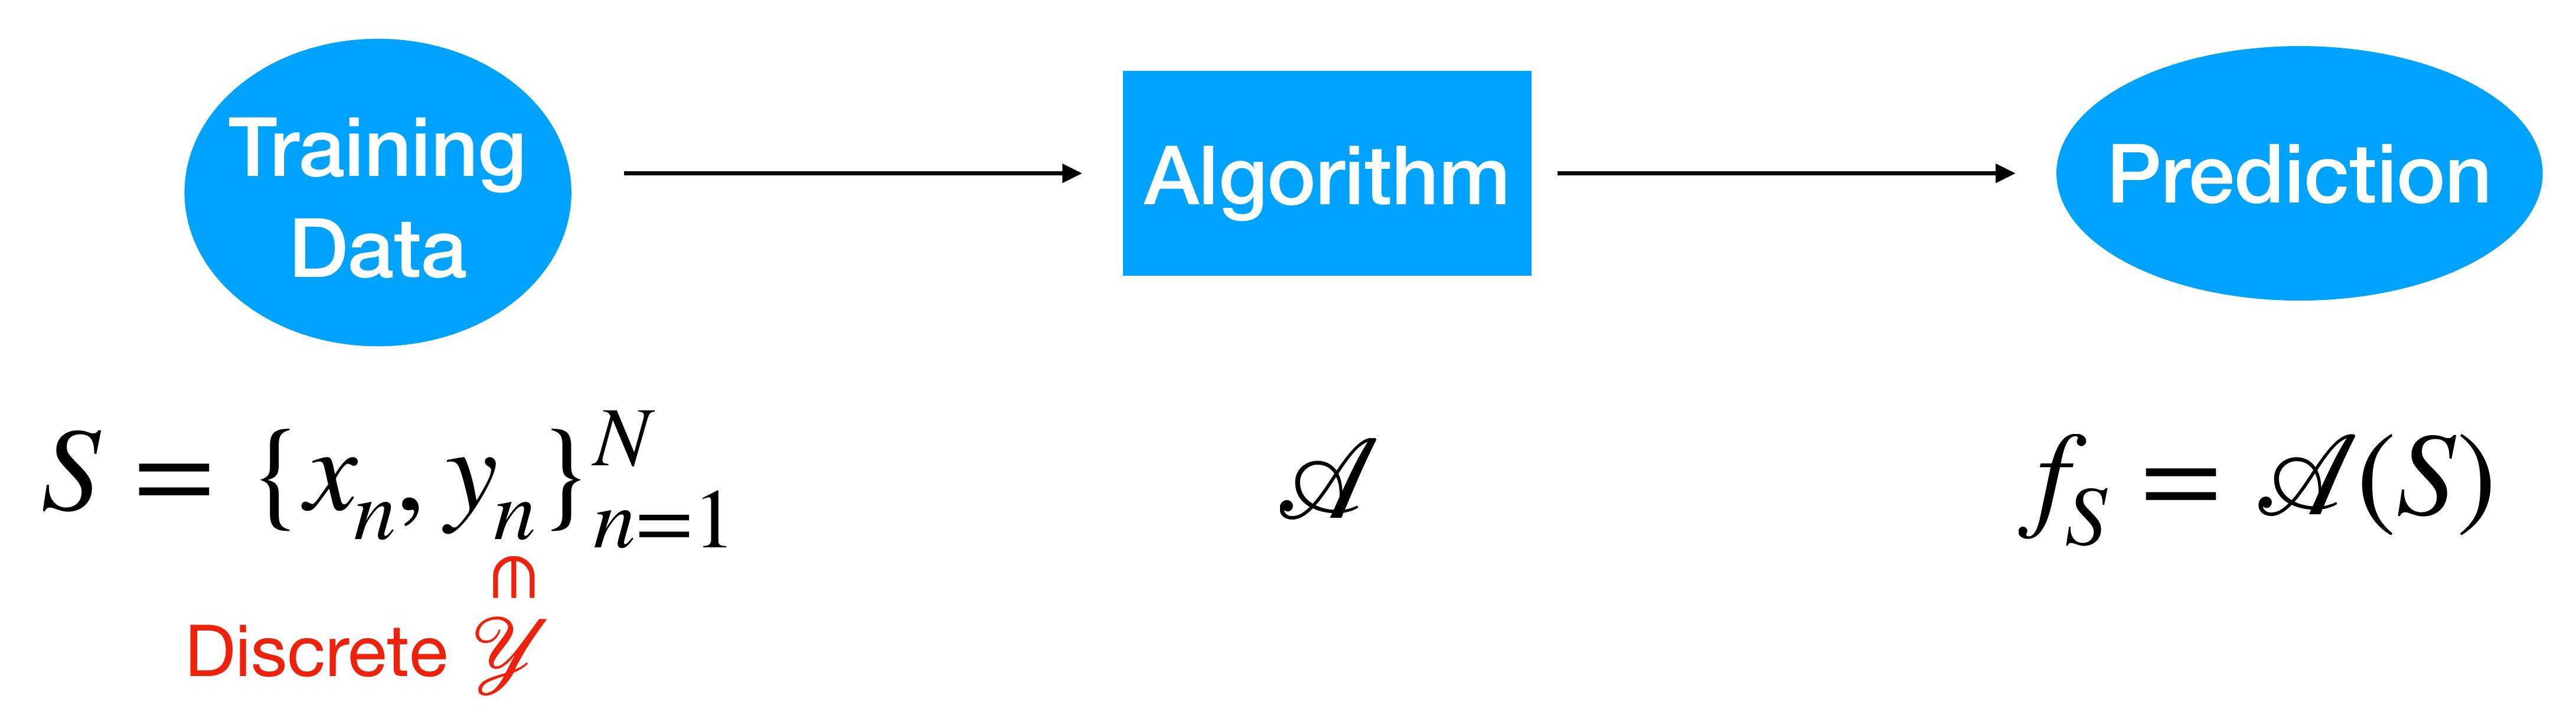
\includegraphics[max width=\textwidth]{2023_12_30_cf784c471dfd1dd5afbag-02}
\end{center}

\section*{Classification: relates input to a categorical variable}
$$
(x, y)=\underbrace{0}_{\text {Discrete Set }} \times \underbrace{0}_{b}
$$

Binary Classification: $y$ can take two values

$y \in\left\{c_{1}, c_{2}\right\}$ where $c_{i}$ are the class labels. We often use $\{0,1\}$ or $\{-1,1\}$

Multi-class classification: $y$ can take more than two values

$y \in\left\{c_{1}, \cdots, c_{K-1}\right\}$ for a $K$ classes problem. We often use $\{0, \cdots, K-1\}$

no ordering between classes

\section*{Spam Detection}
\begin{center}
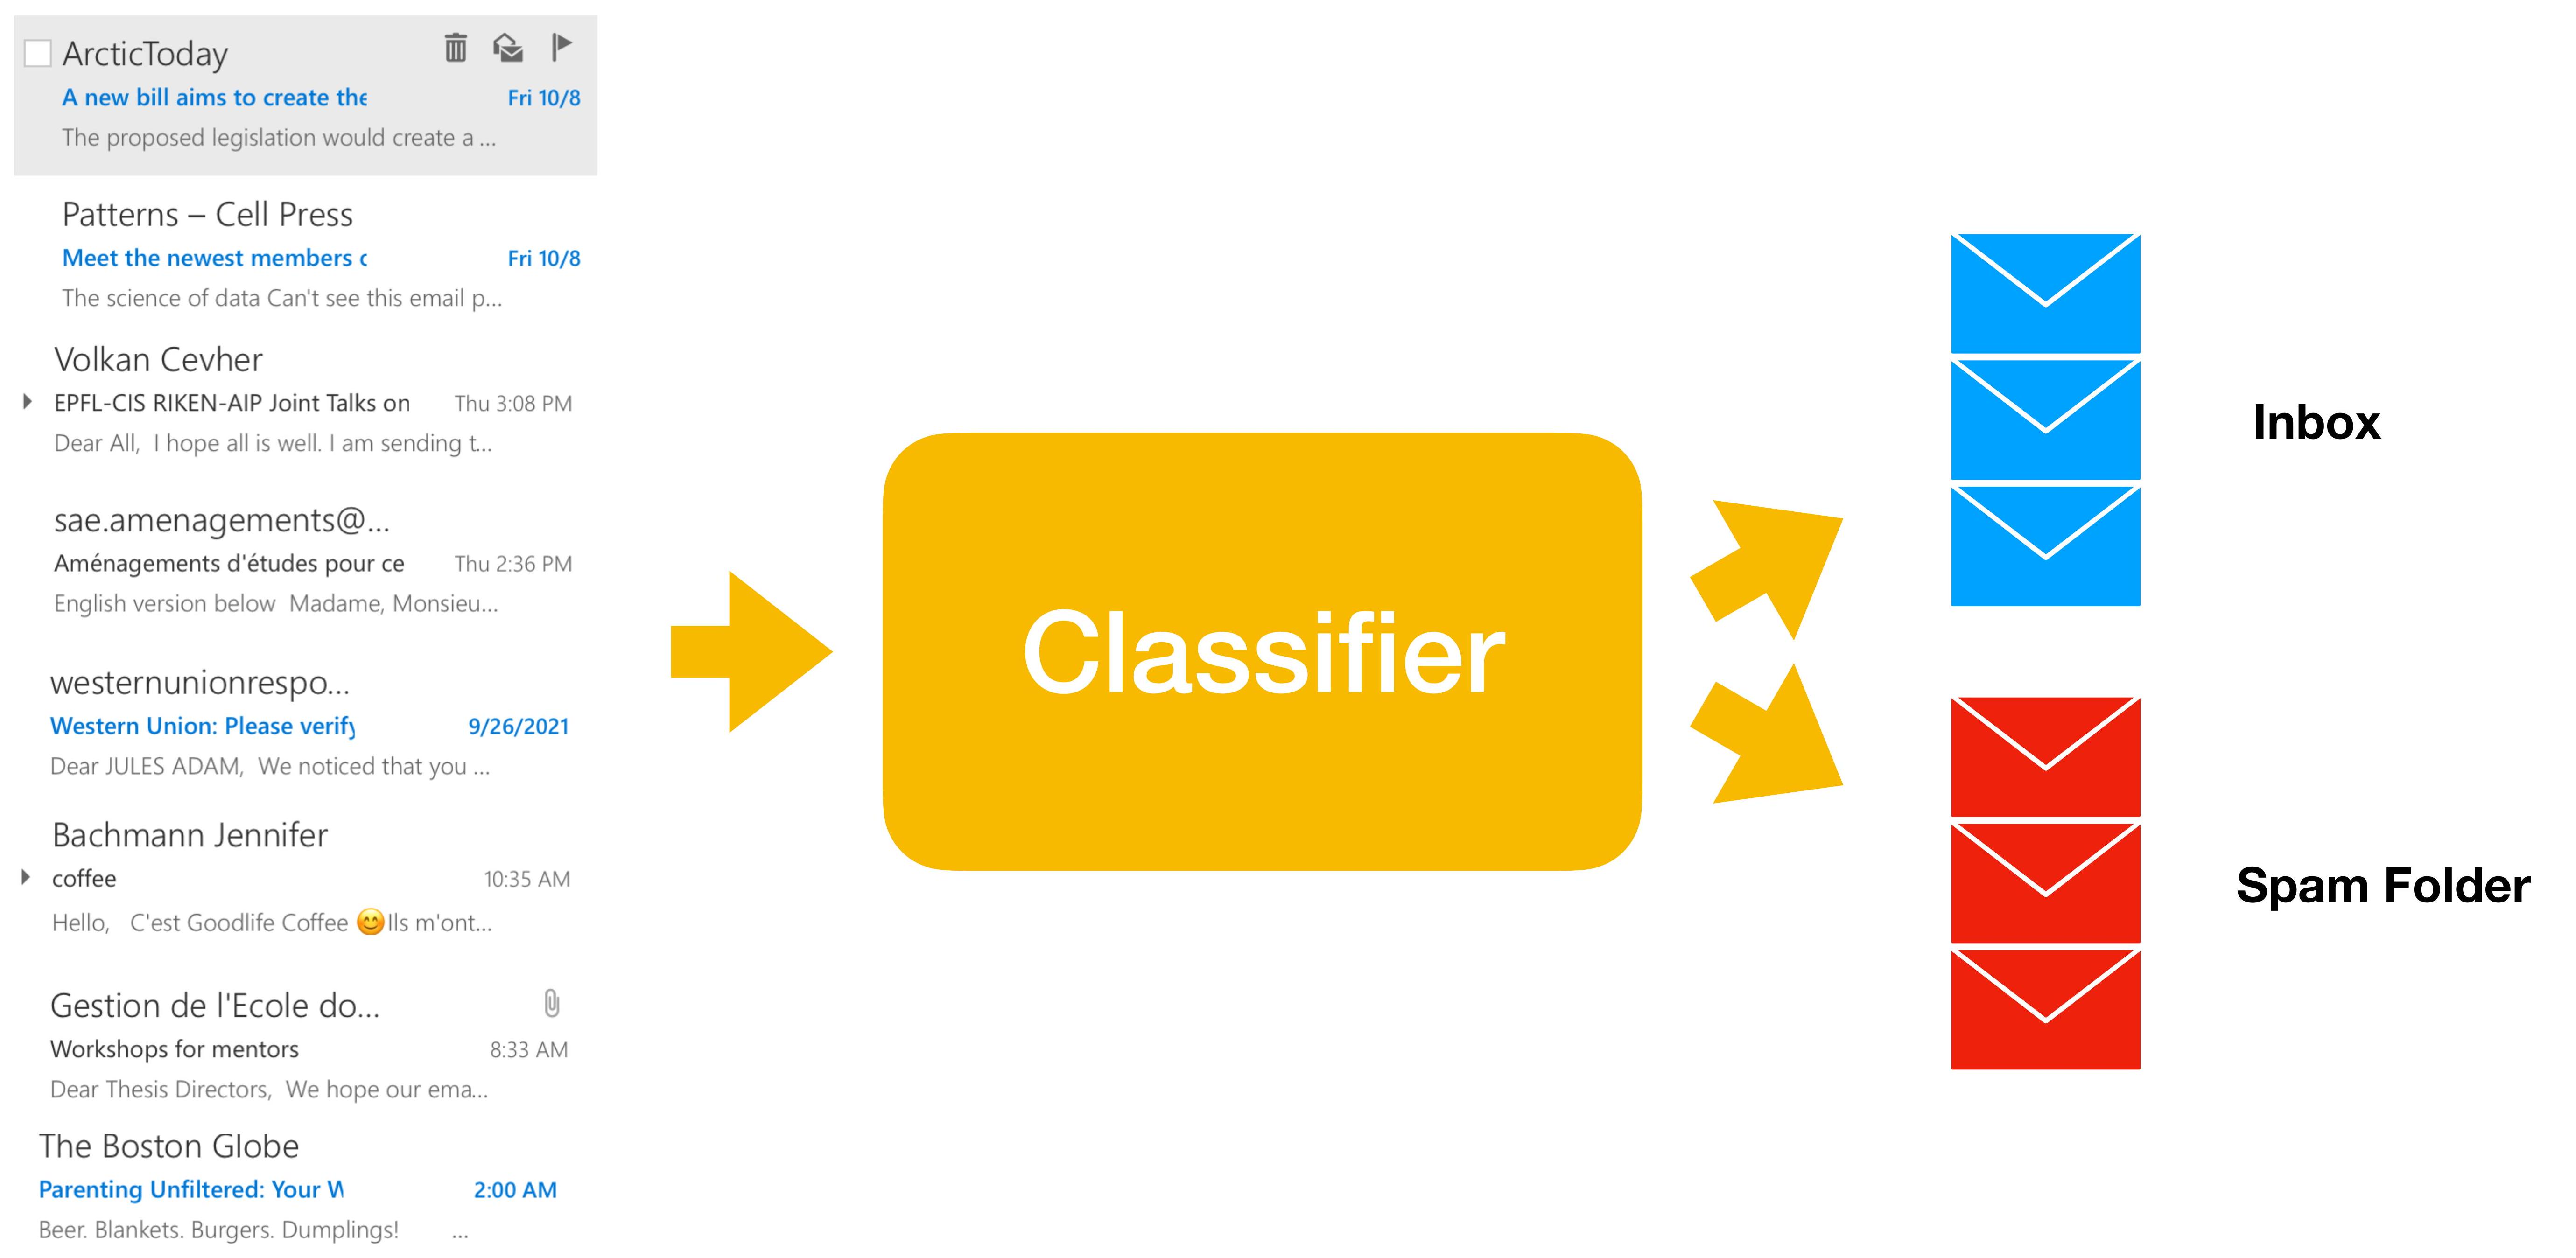
\includegraphics[max width=\textwidth]{2023_12_30_cf784c471dfd1dd5afbag-04}
\end{center}

\section*{Image classification}
\begin{center}
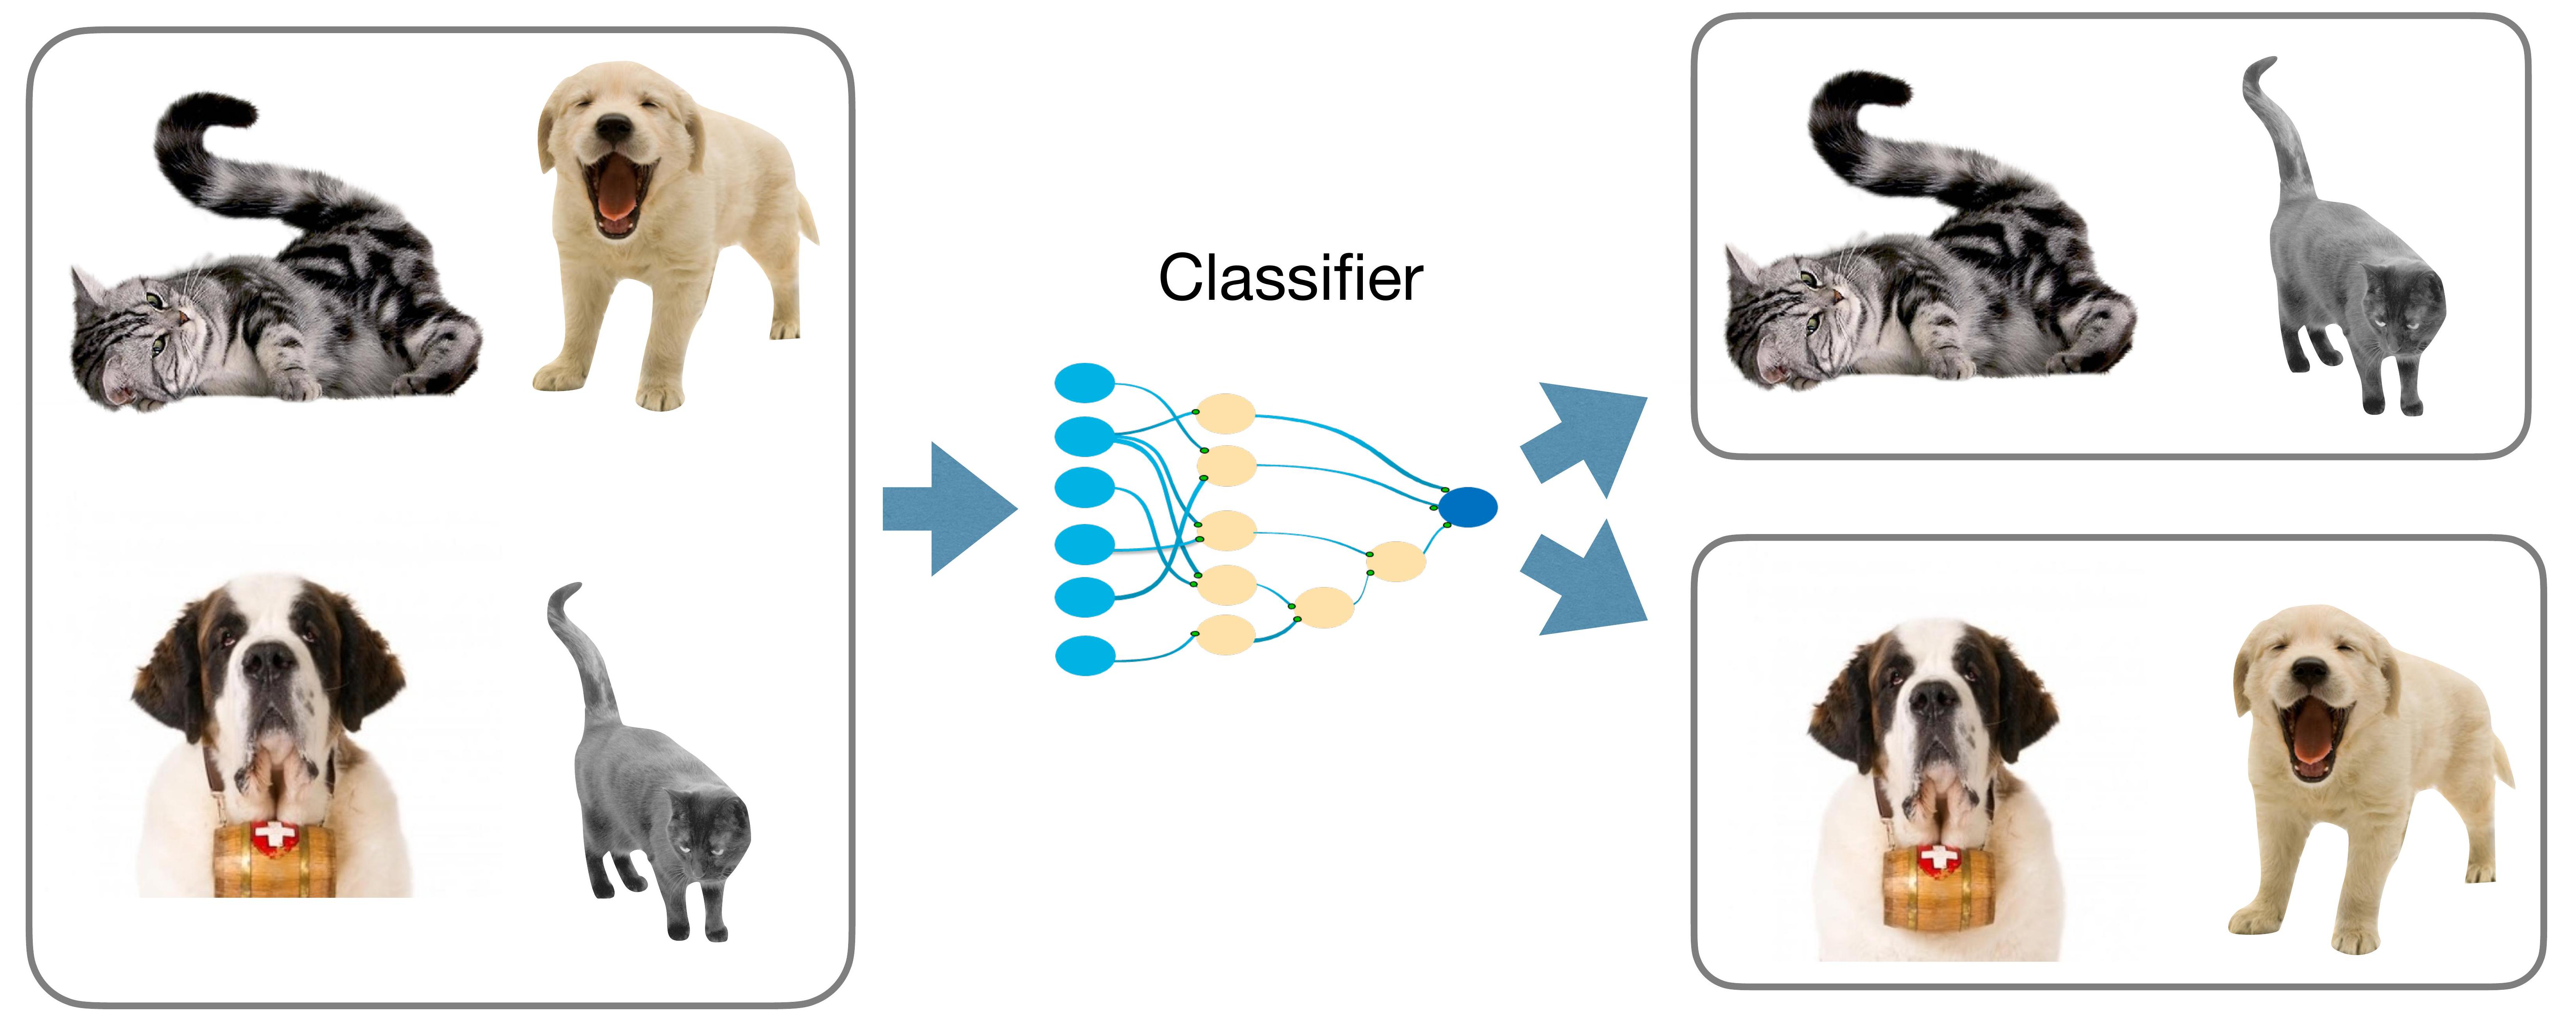
\includegraphics[max width=\textwidth]{2023_12_30_cf784c471dfd1dd5afbag-05}
\end{center}

\section*{Credit Card Default}
\begin{center}
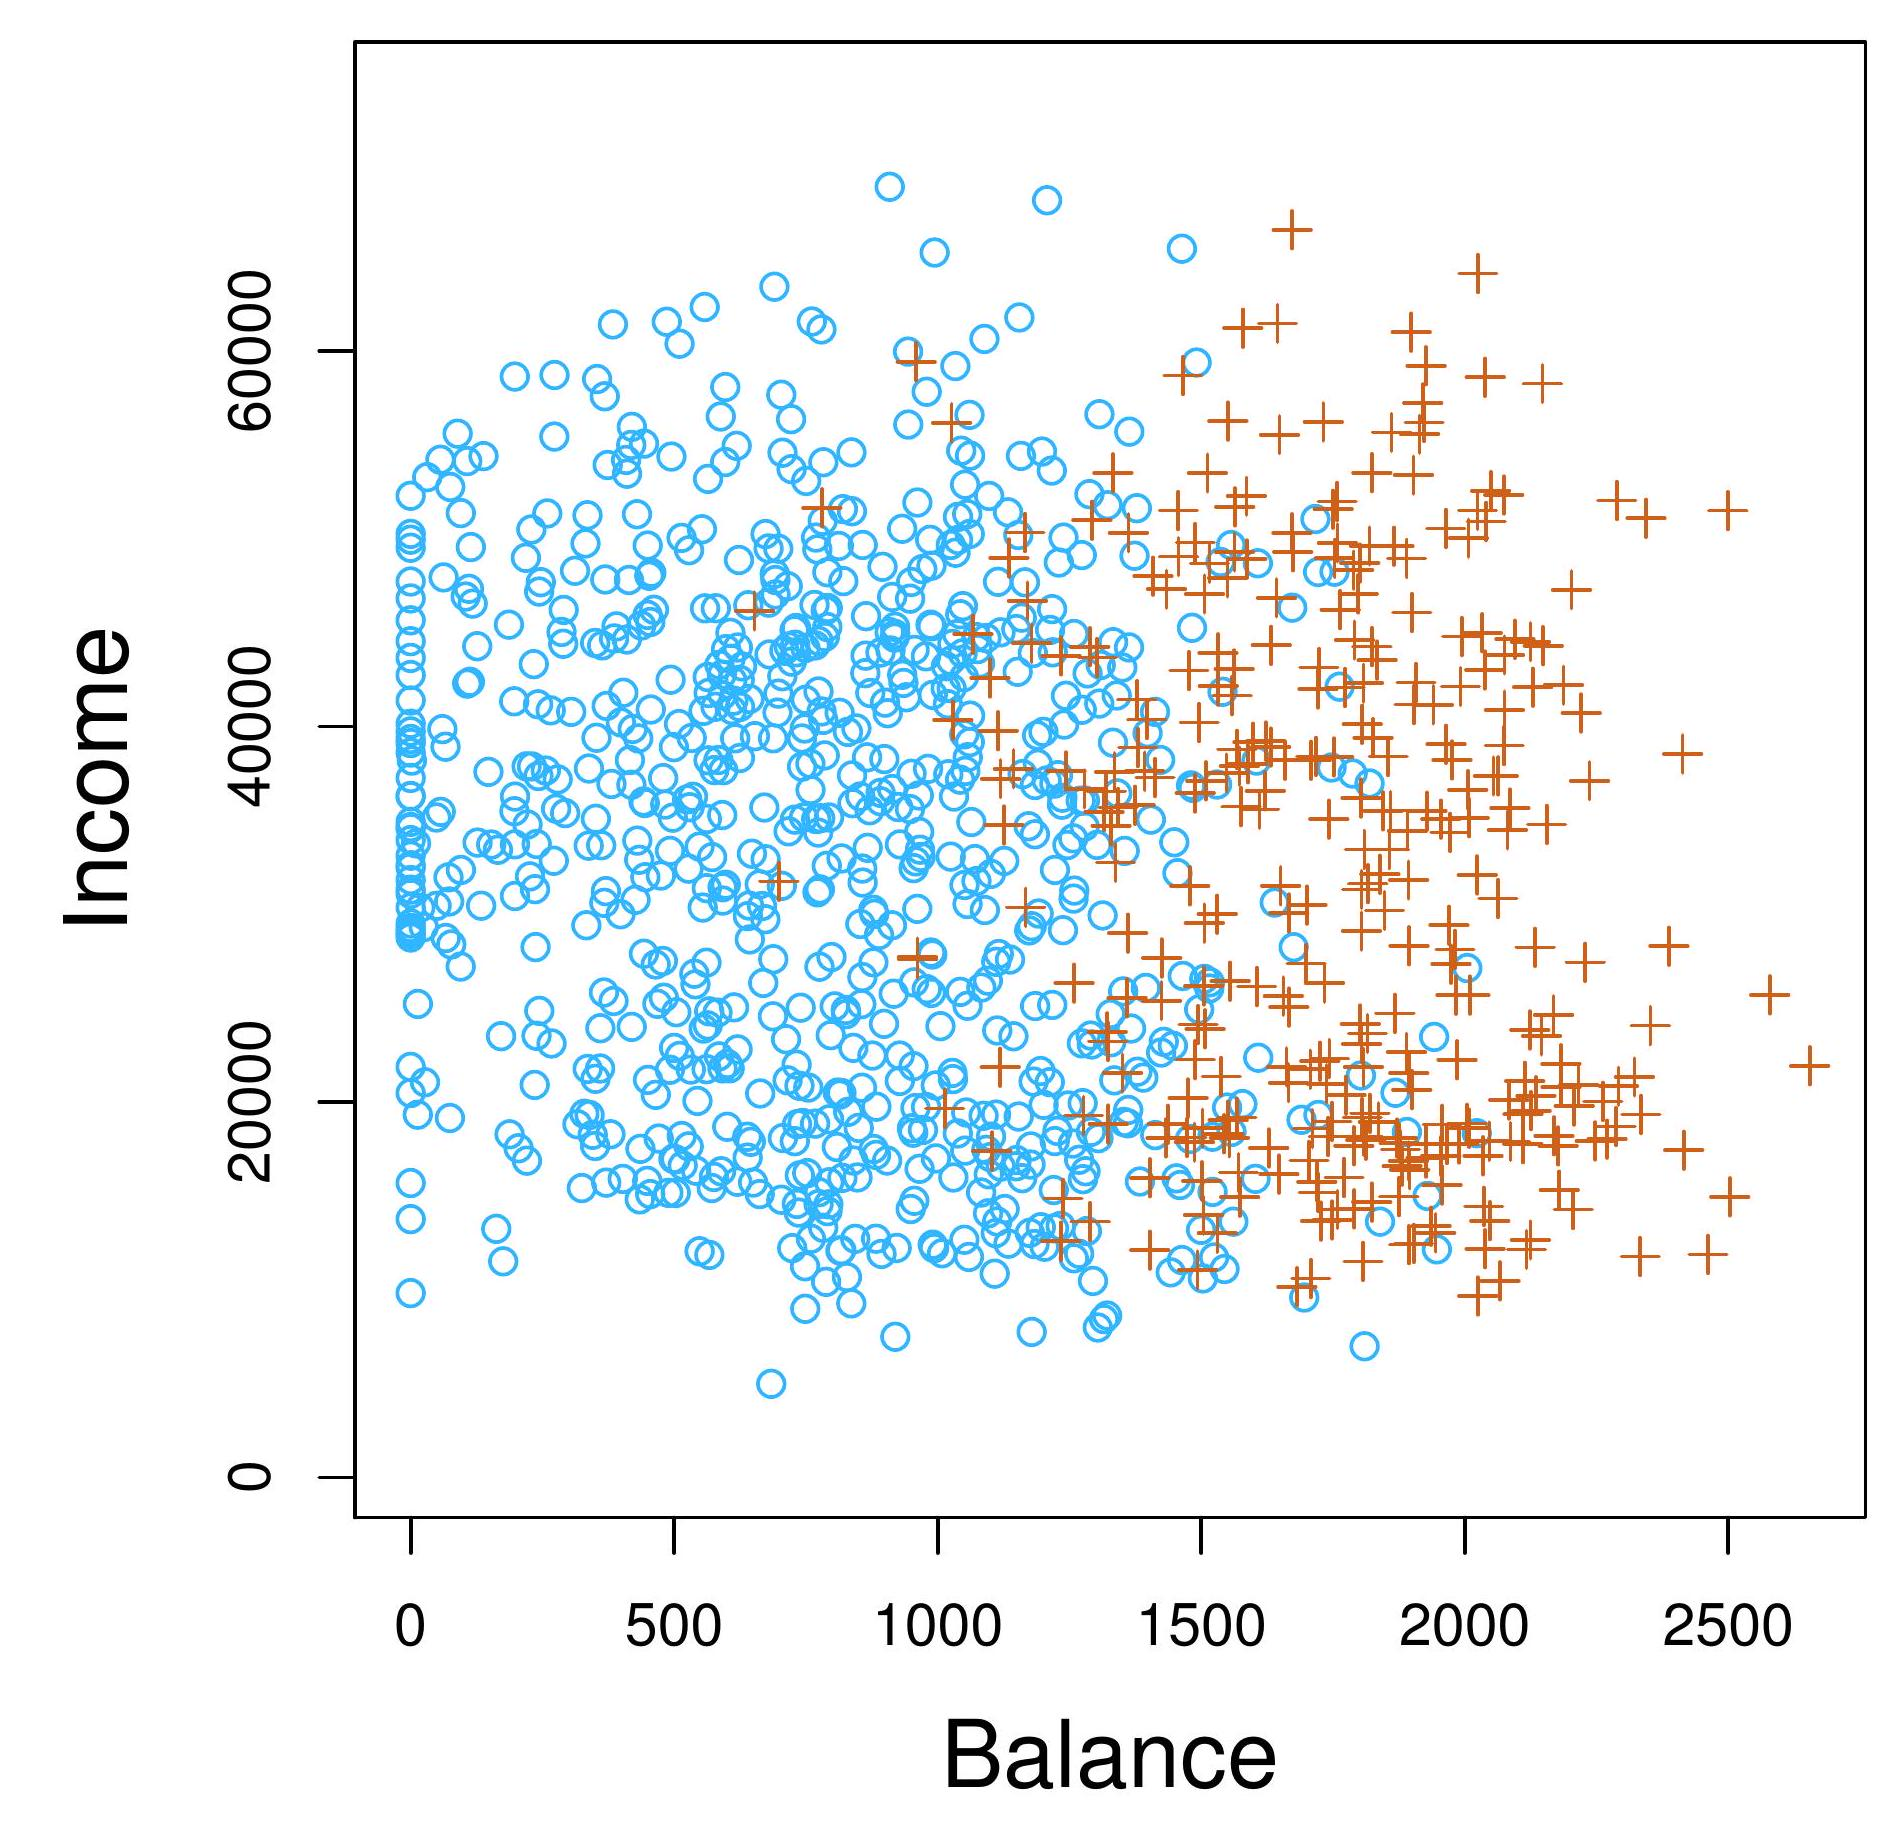
\includegraphics[max width=\textwidth]{2023_12_30_cf784c471dfd1dd5afbag-06}
\end{center}

\begin{itemize}
  \item individual who defaulted on their credit card payments individual who did not
\end{itemize}

\section*{Classifier}
A classifier $f: \mathscr{X} \rightarrow \mathscr{Y}$ divides the input space into a collection of regions belonging to each class

\begin{center}
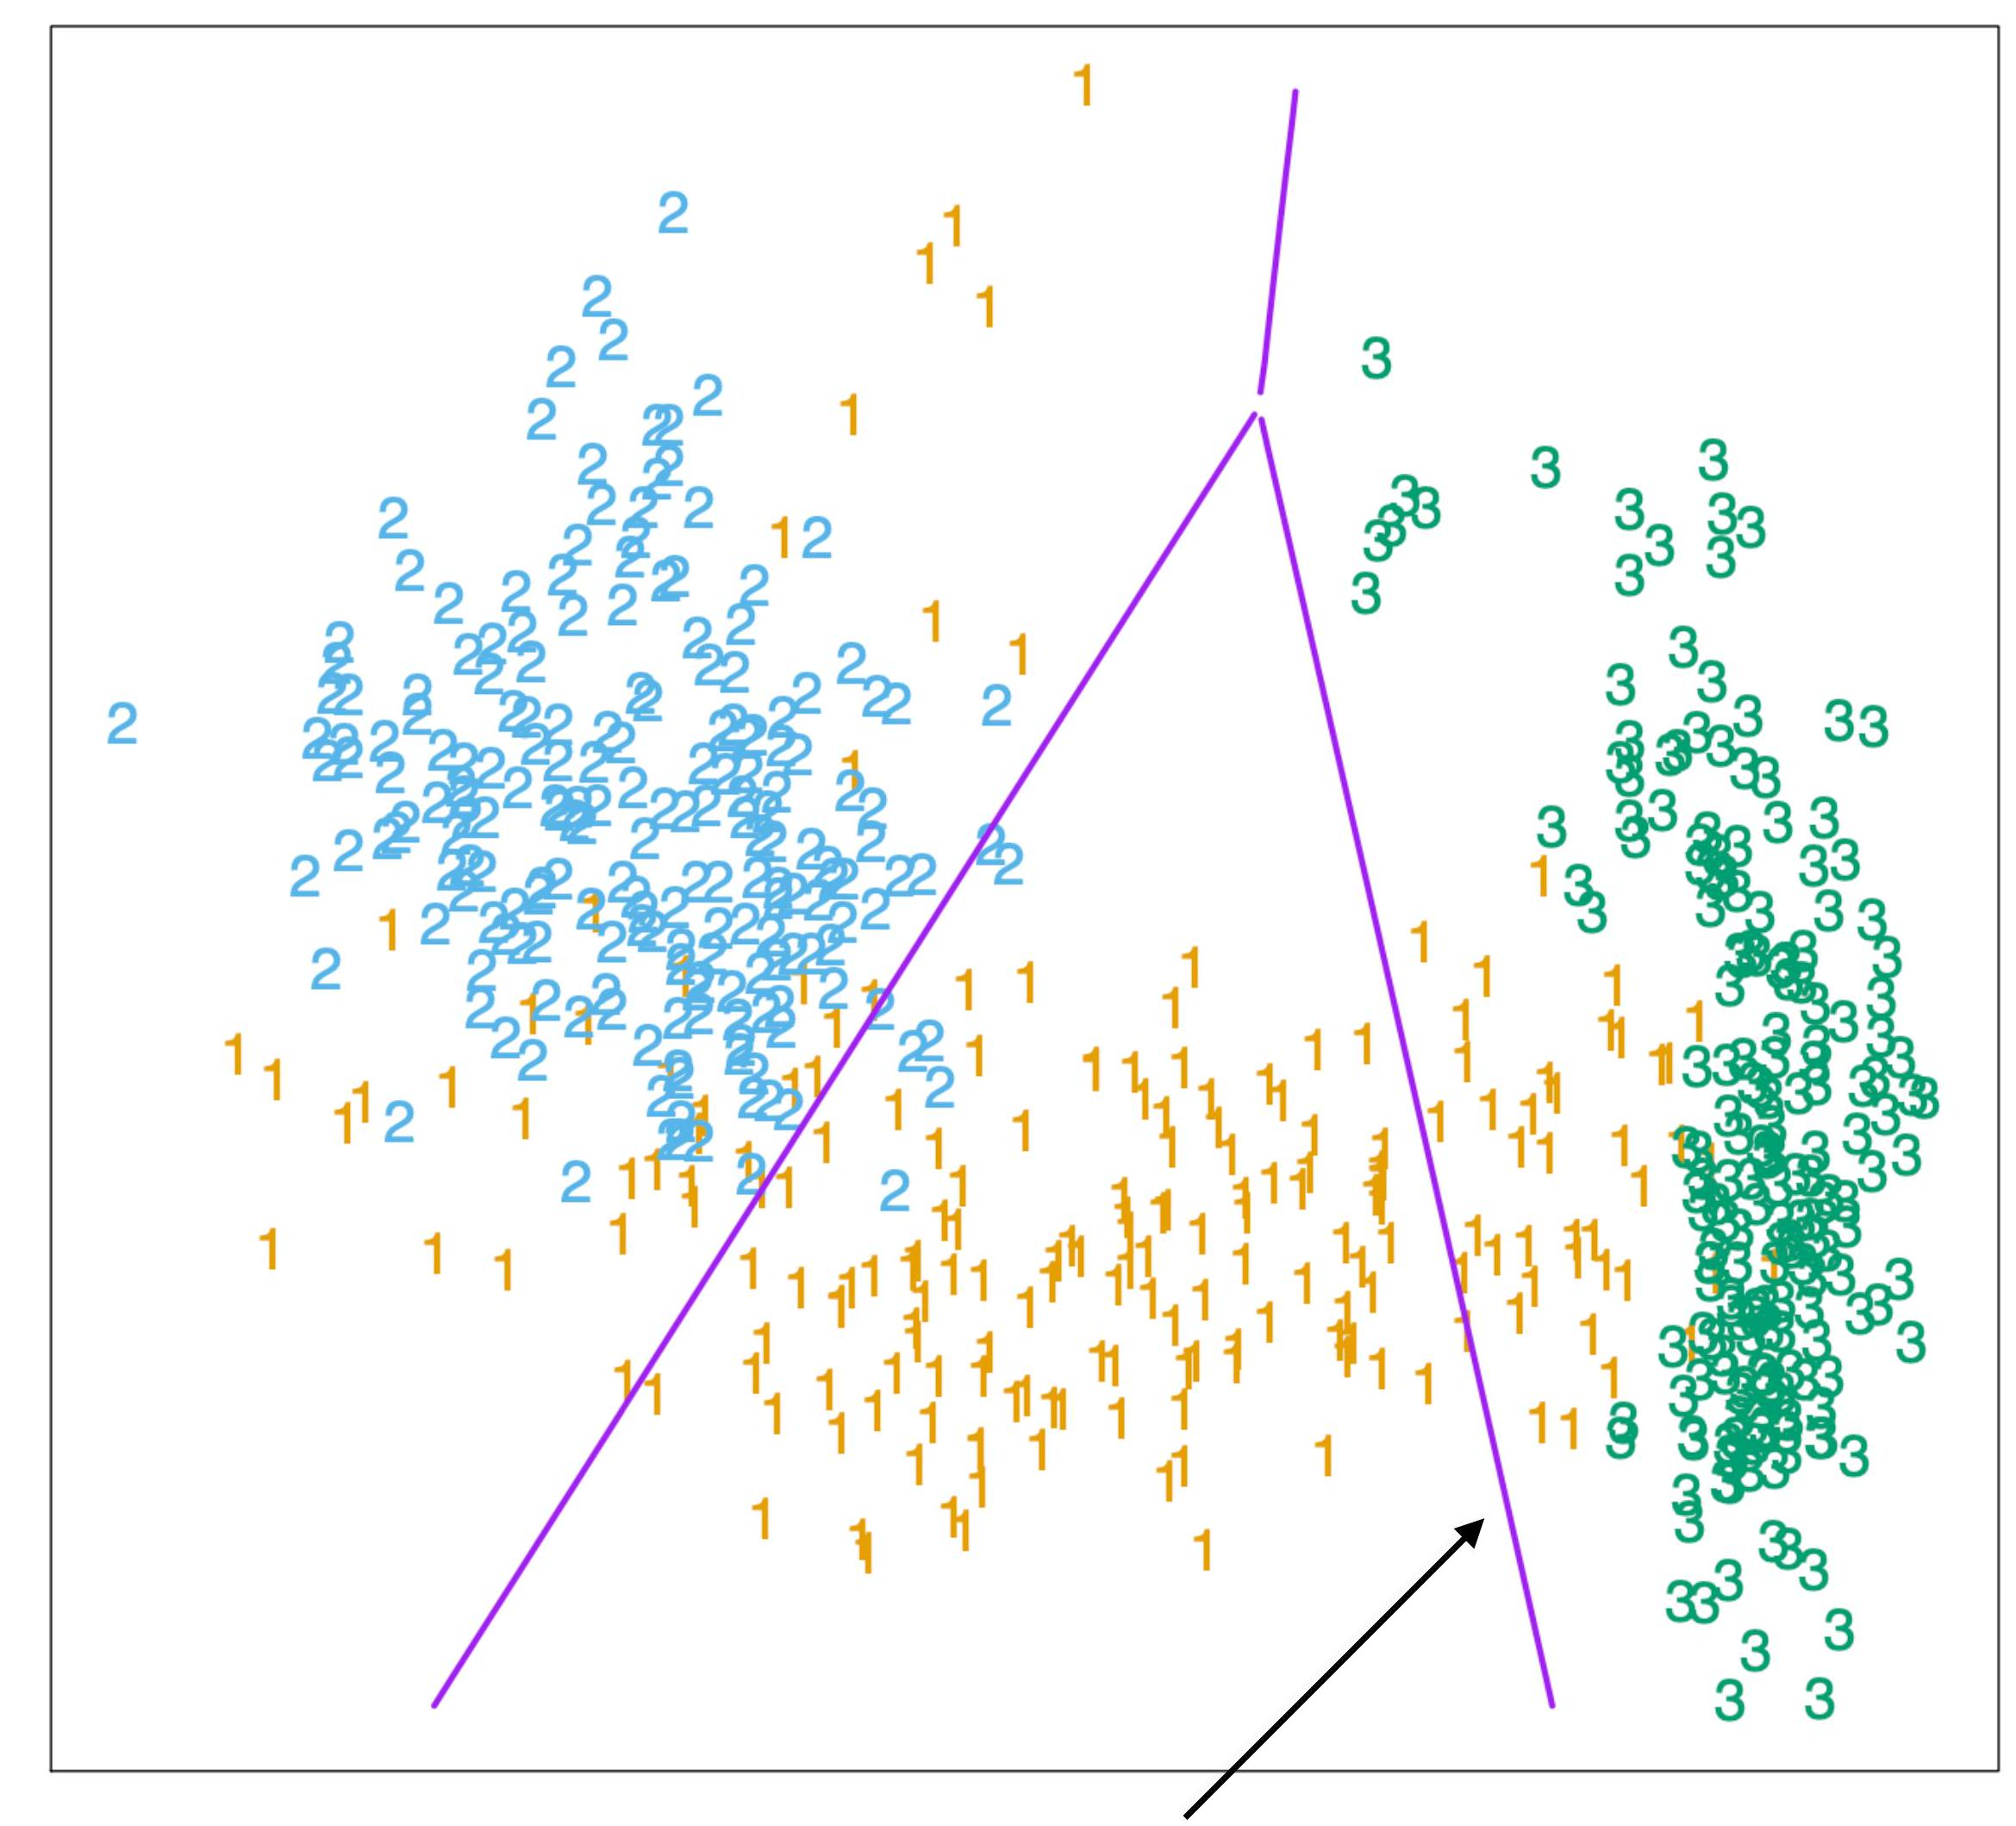
\includegraphics[max width=\textwidth]{2023_12_30_cf784c471dfd1dd5afbag-07}
\end{center}

\section*{Classifier}
A classifier $f: \mathscr{X} \rightarrow \mathcal{Y}$ divides the input space into a collection of regions belonging to each class

It can be linear

\begin{center}
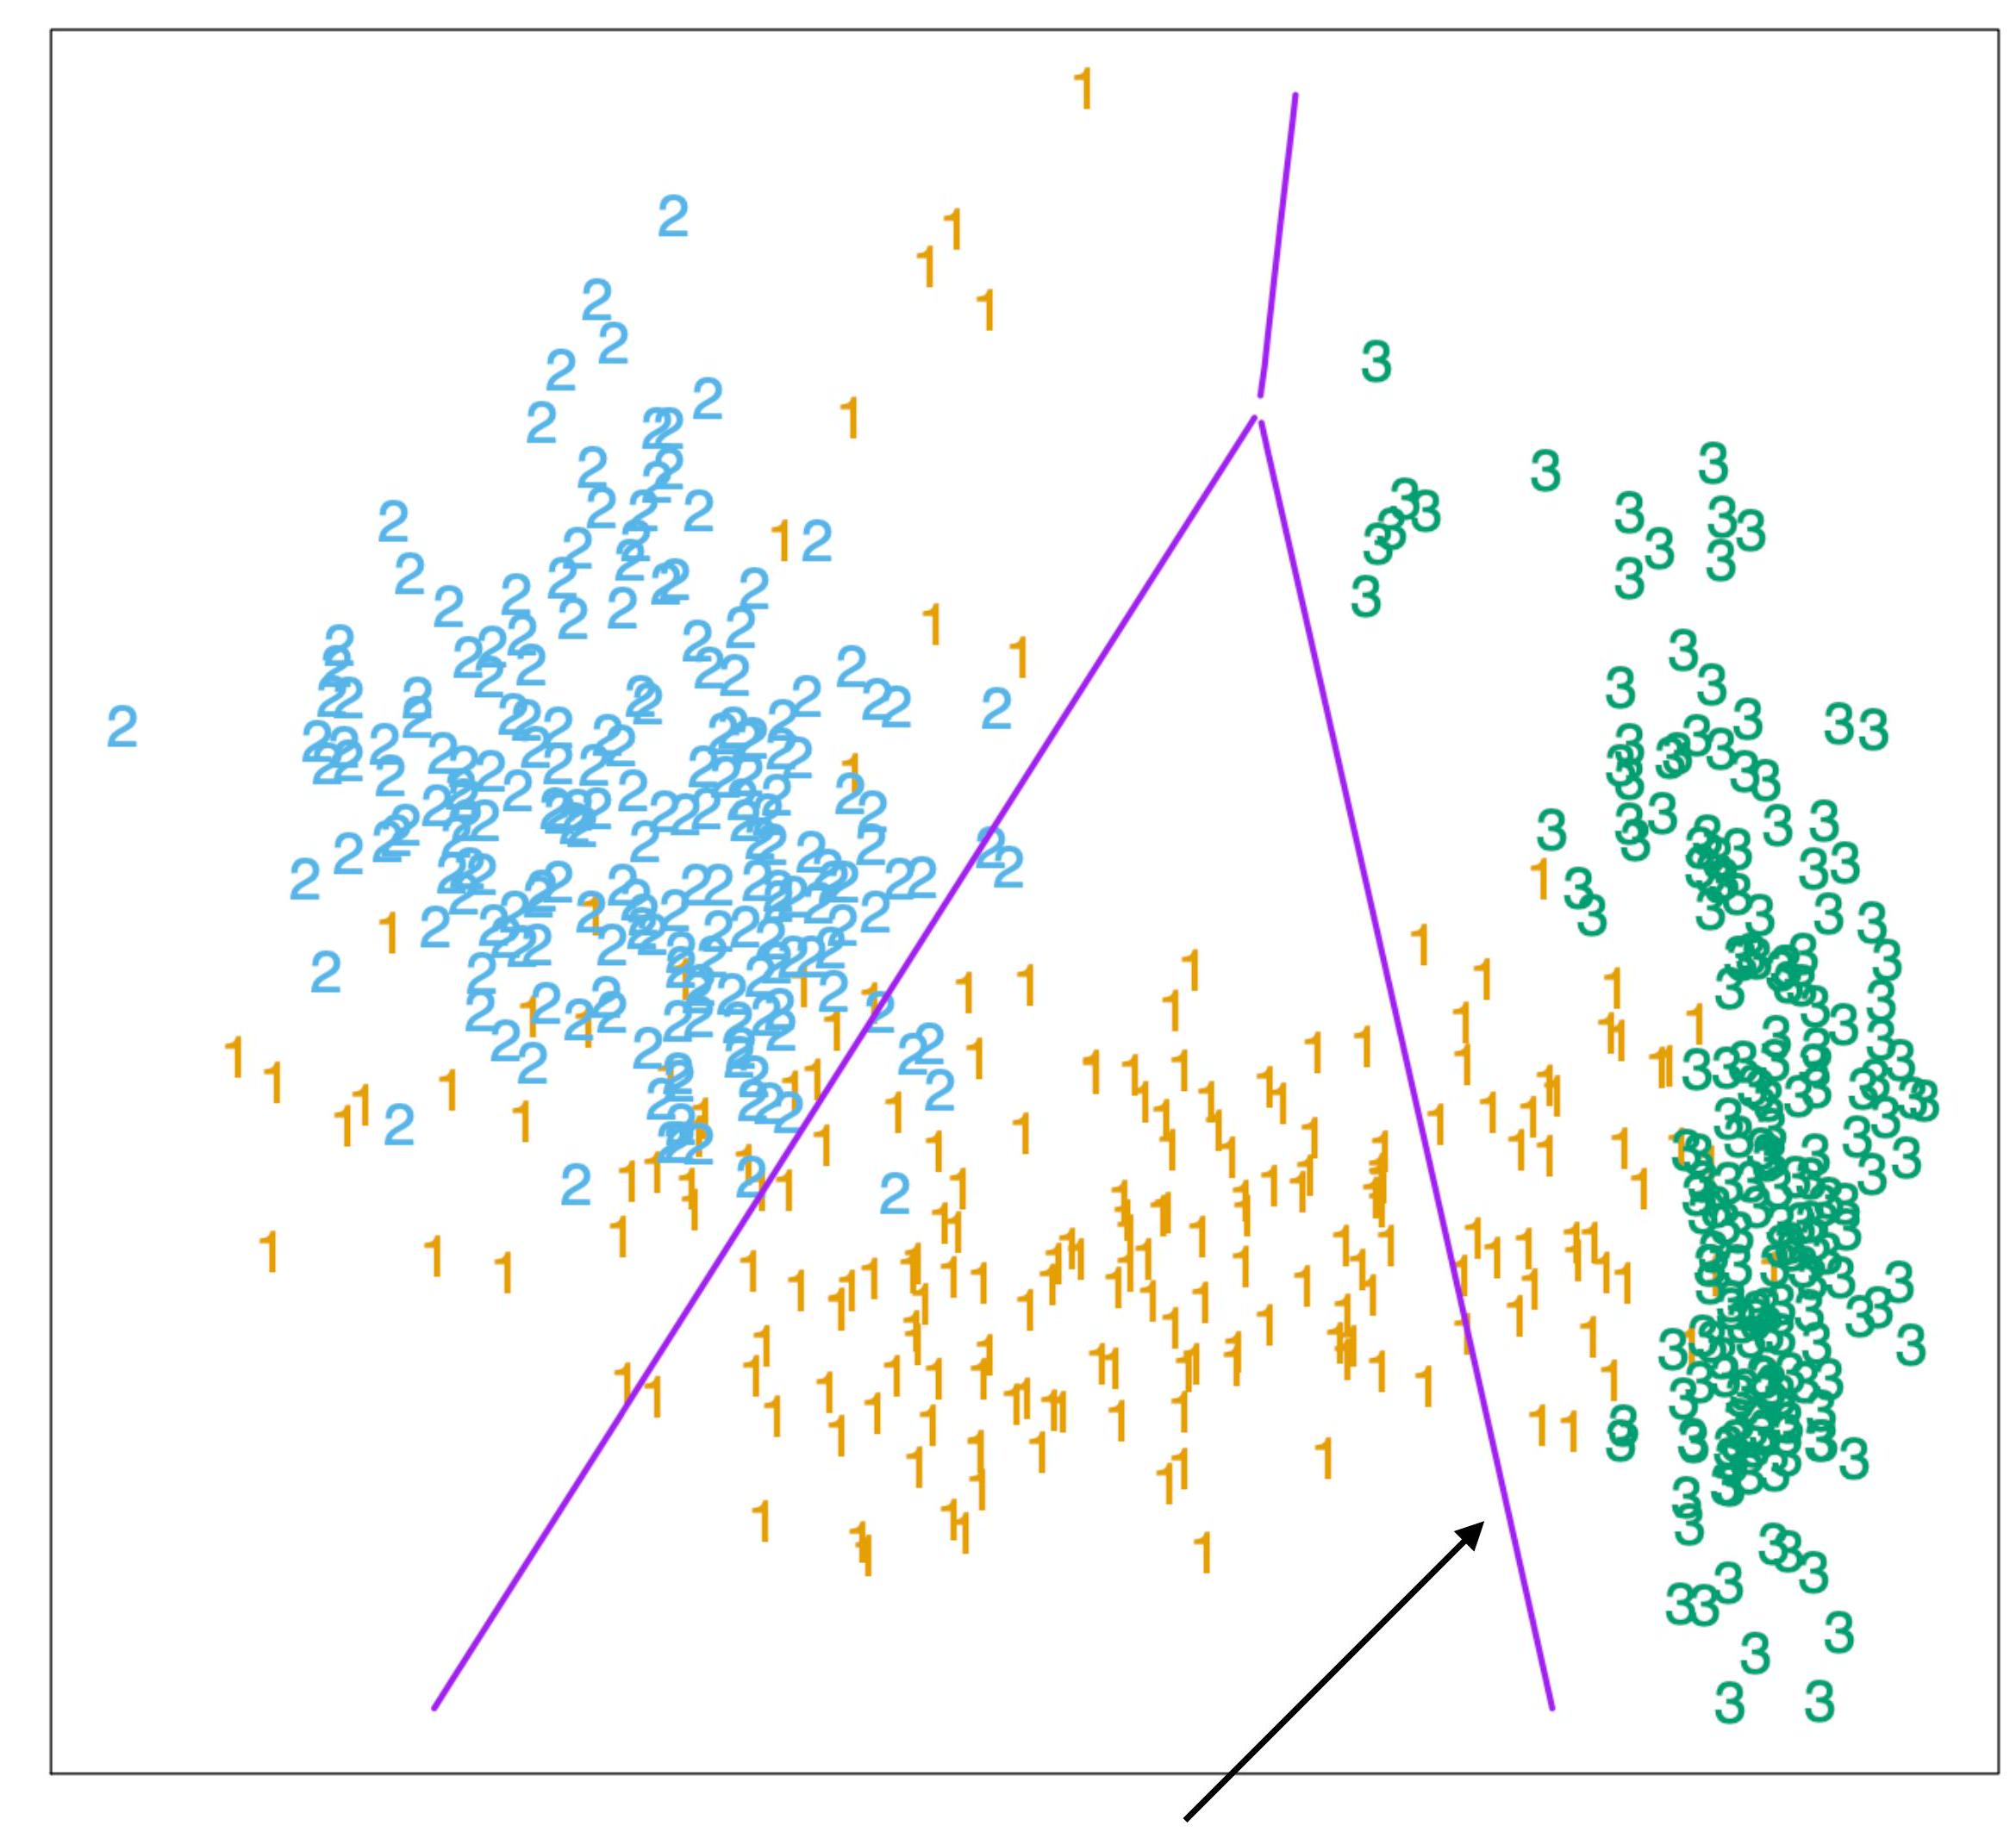
\includegraphics[max width=\textwidth]{2023_12_30_cf784c471dfd1dd5afbag-08}
\end{center}

Linear Decision boundary

\section*{Classifier}
A classifier $f: \mathscr{X} \rightarrow \mathcal{Y}$ divides the input space into a collection of regions belonging to each class

It can also be nonlinear

\begin{center}
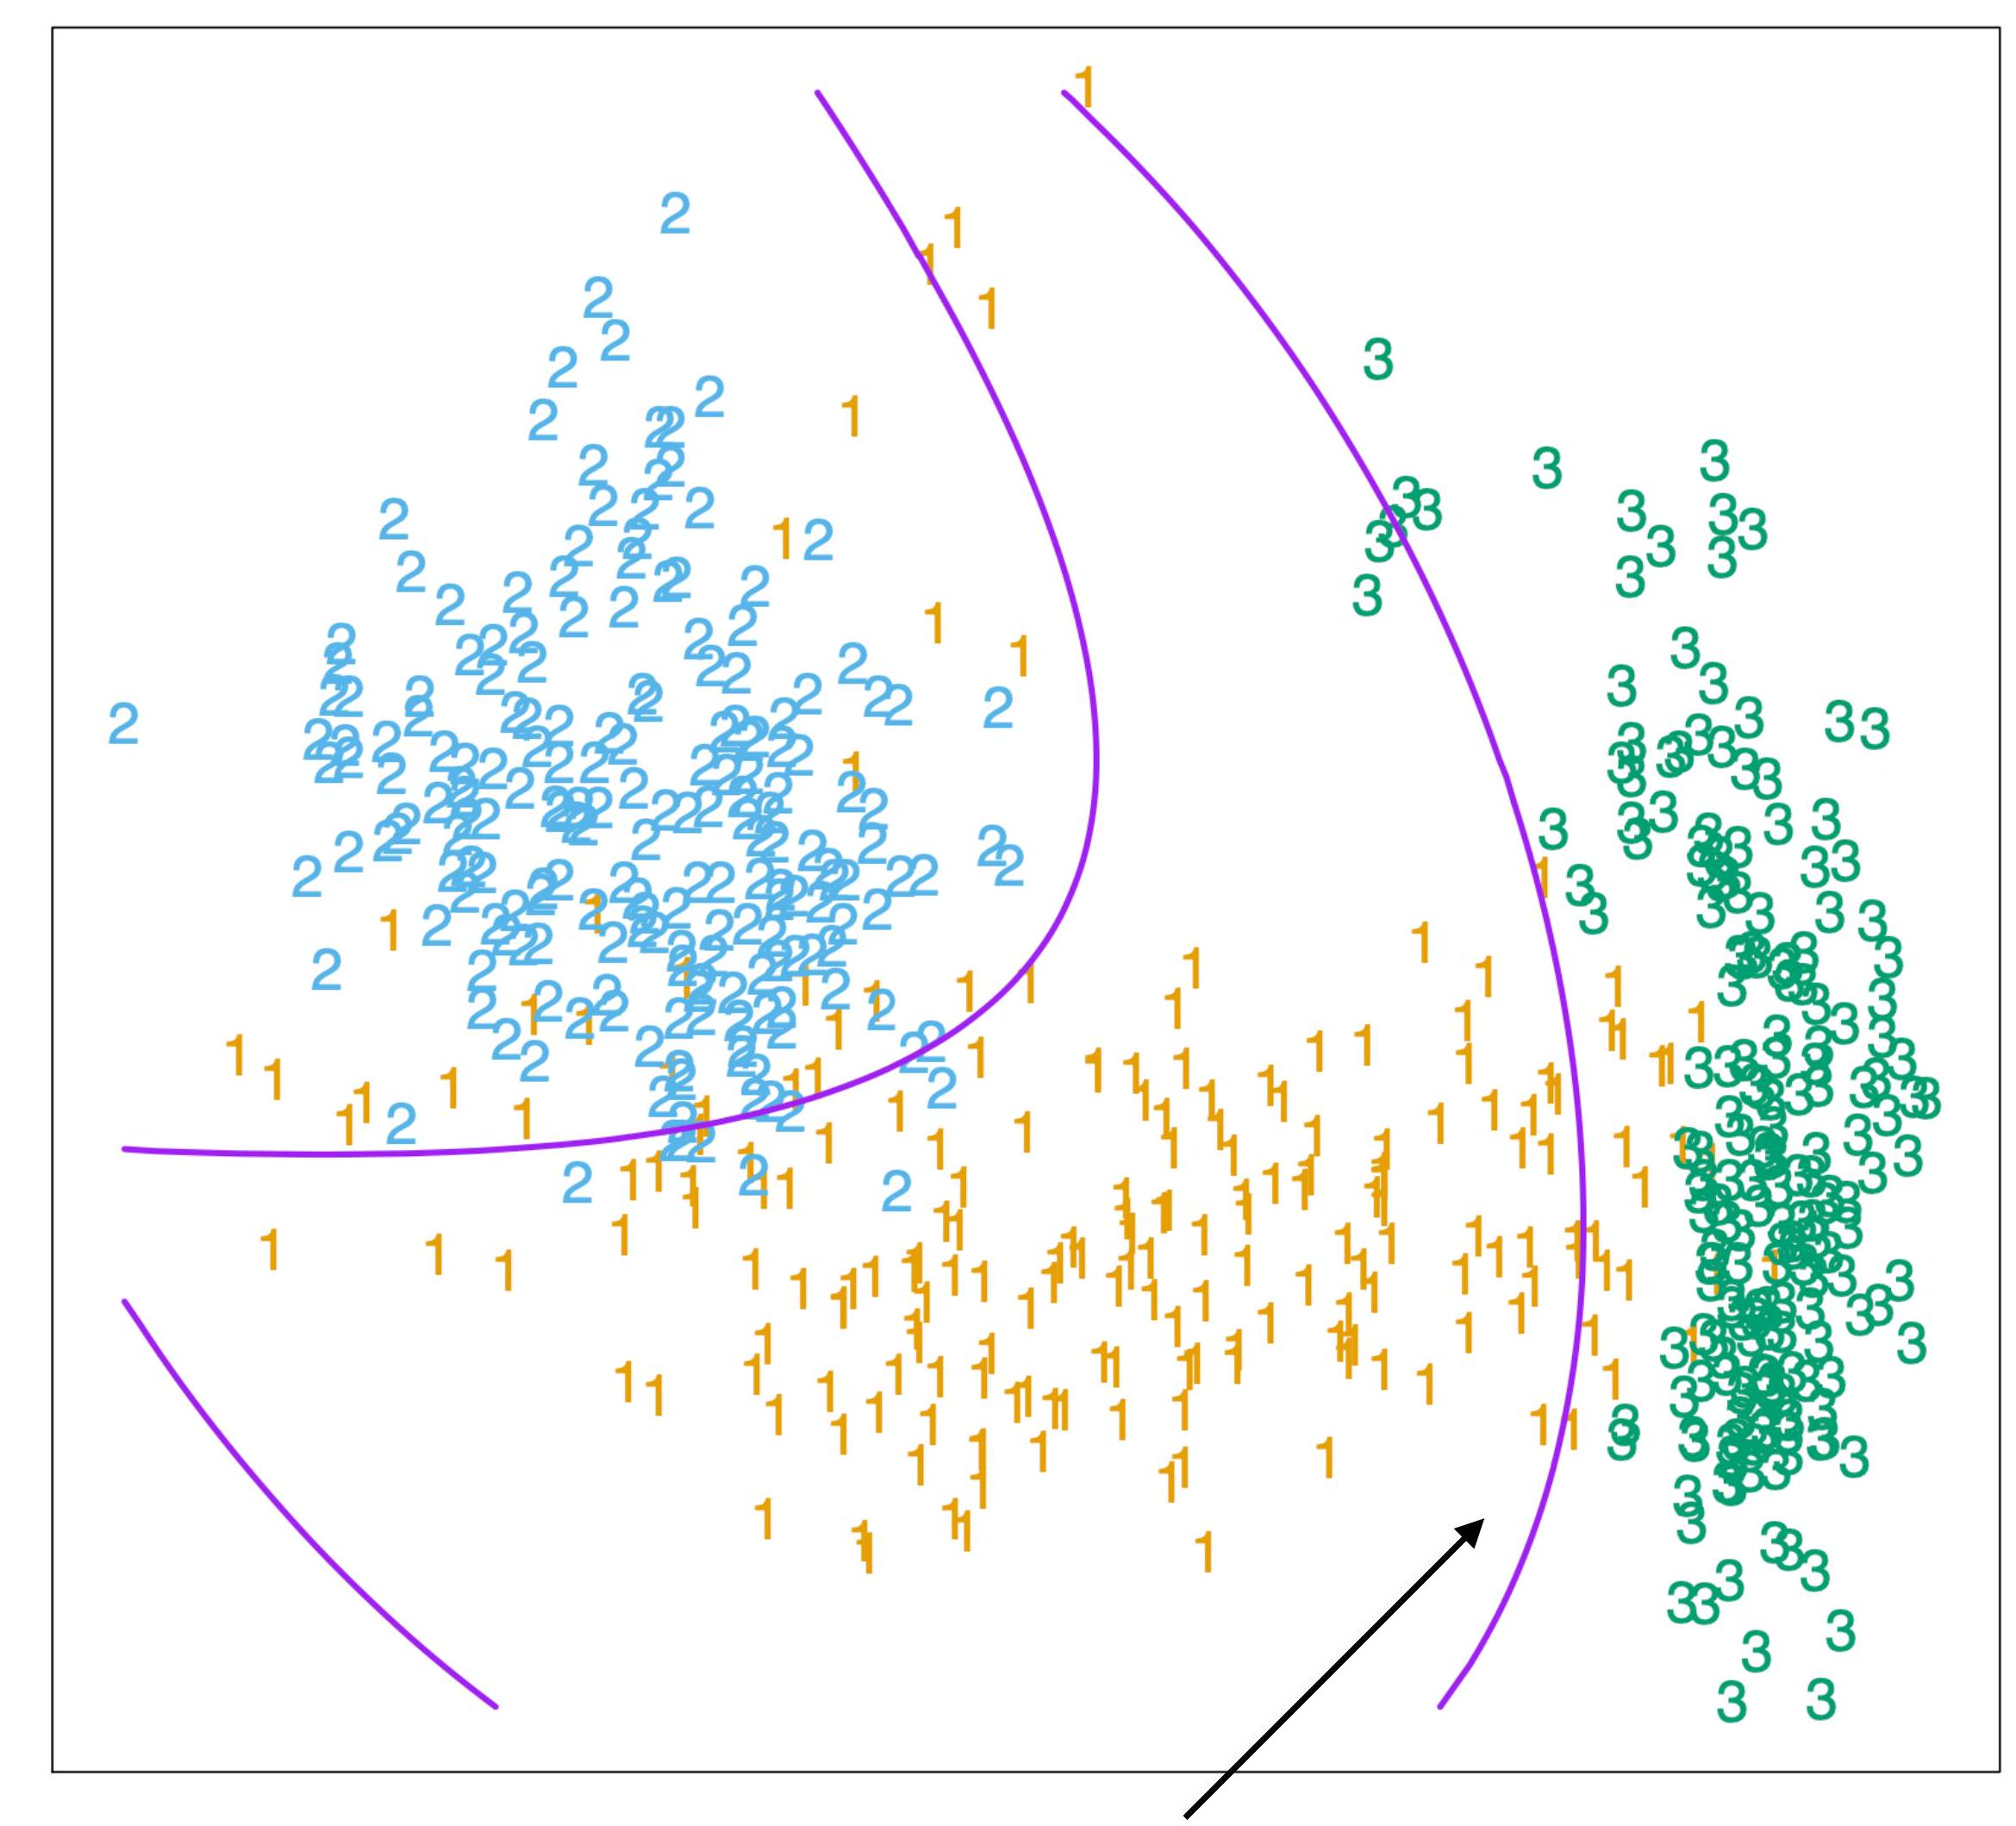
\includegraphics[max width=\textwidth]{2023_12_30_cf784c471dfd1dd5afbag-09}
\end{center}

\section*{Classification: a special case of regression?}
Classification is a regression problem with discrete labels:

$$
(x, y) \in \mathscr{X} \times\{0,1\} \subset \mathscr{X} \times \mathbb{R}
$$

Could we use previously seen regression methods to solve it?

\section*{Classification: a special case of regression?}
Classification is a regression problem with discrete labels:

$$
(x, y) \in \mathscr{X} \times\{0,1\} \subset \mathscr{X} \times \mathbb{R}
$$

Could we use previously seen regression methods to solve it?

\begin{center}
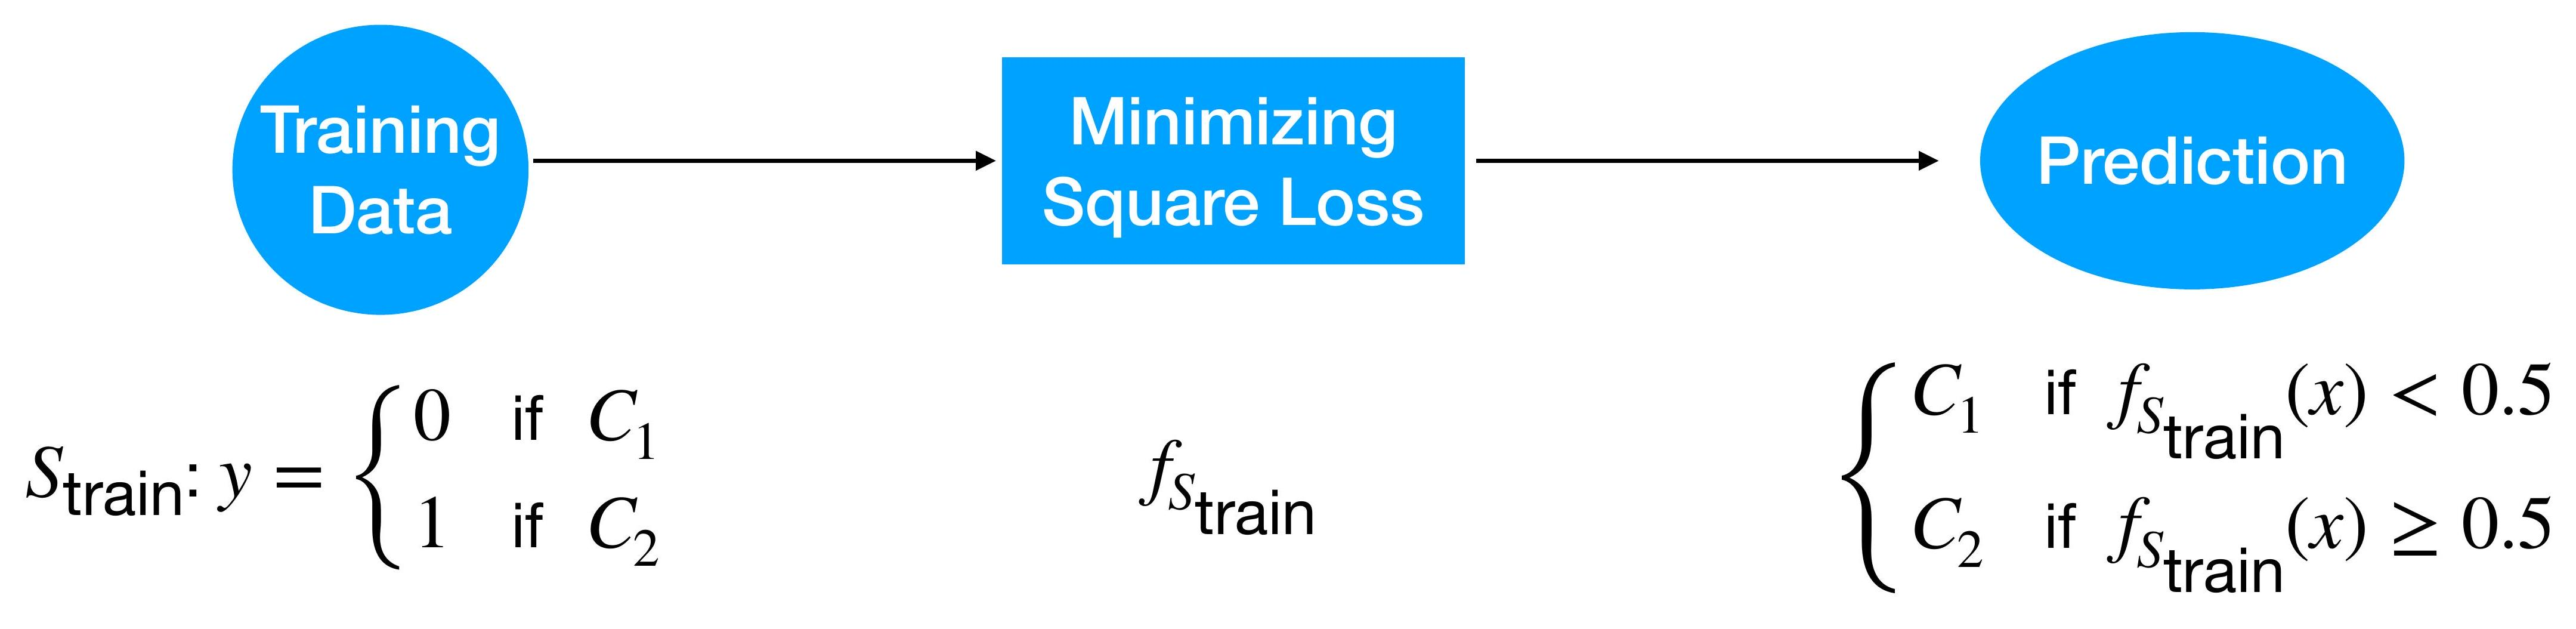
\includegraphics[max width=\textwidth]{2023_12_30_cf784c471dfd1dd5afbag-11}
\end{center}

\section*{Is it a good idea?}
Credit-card default problem:

We label the output as probability for sake of interpretation

\begin{center}
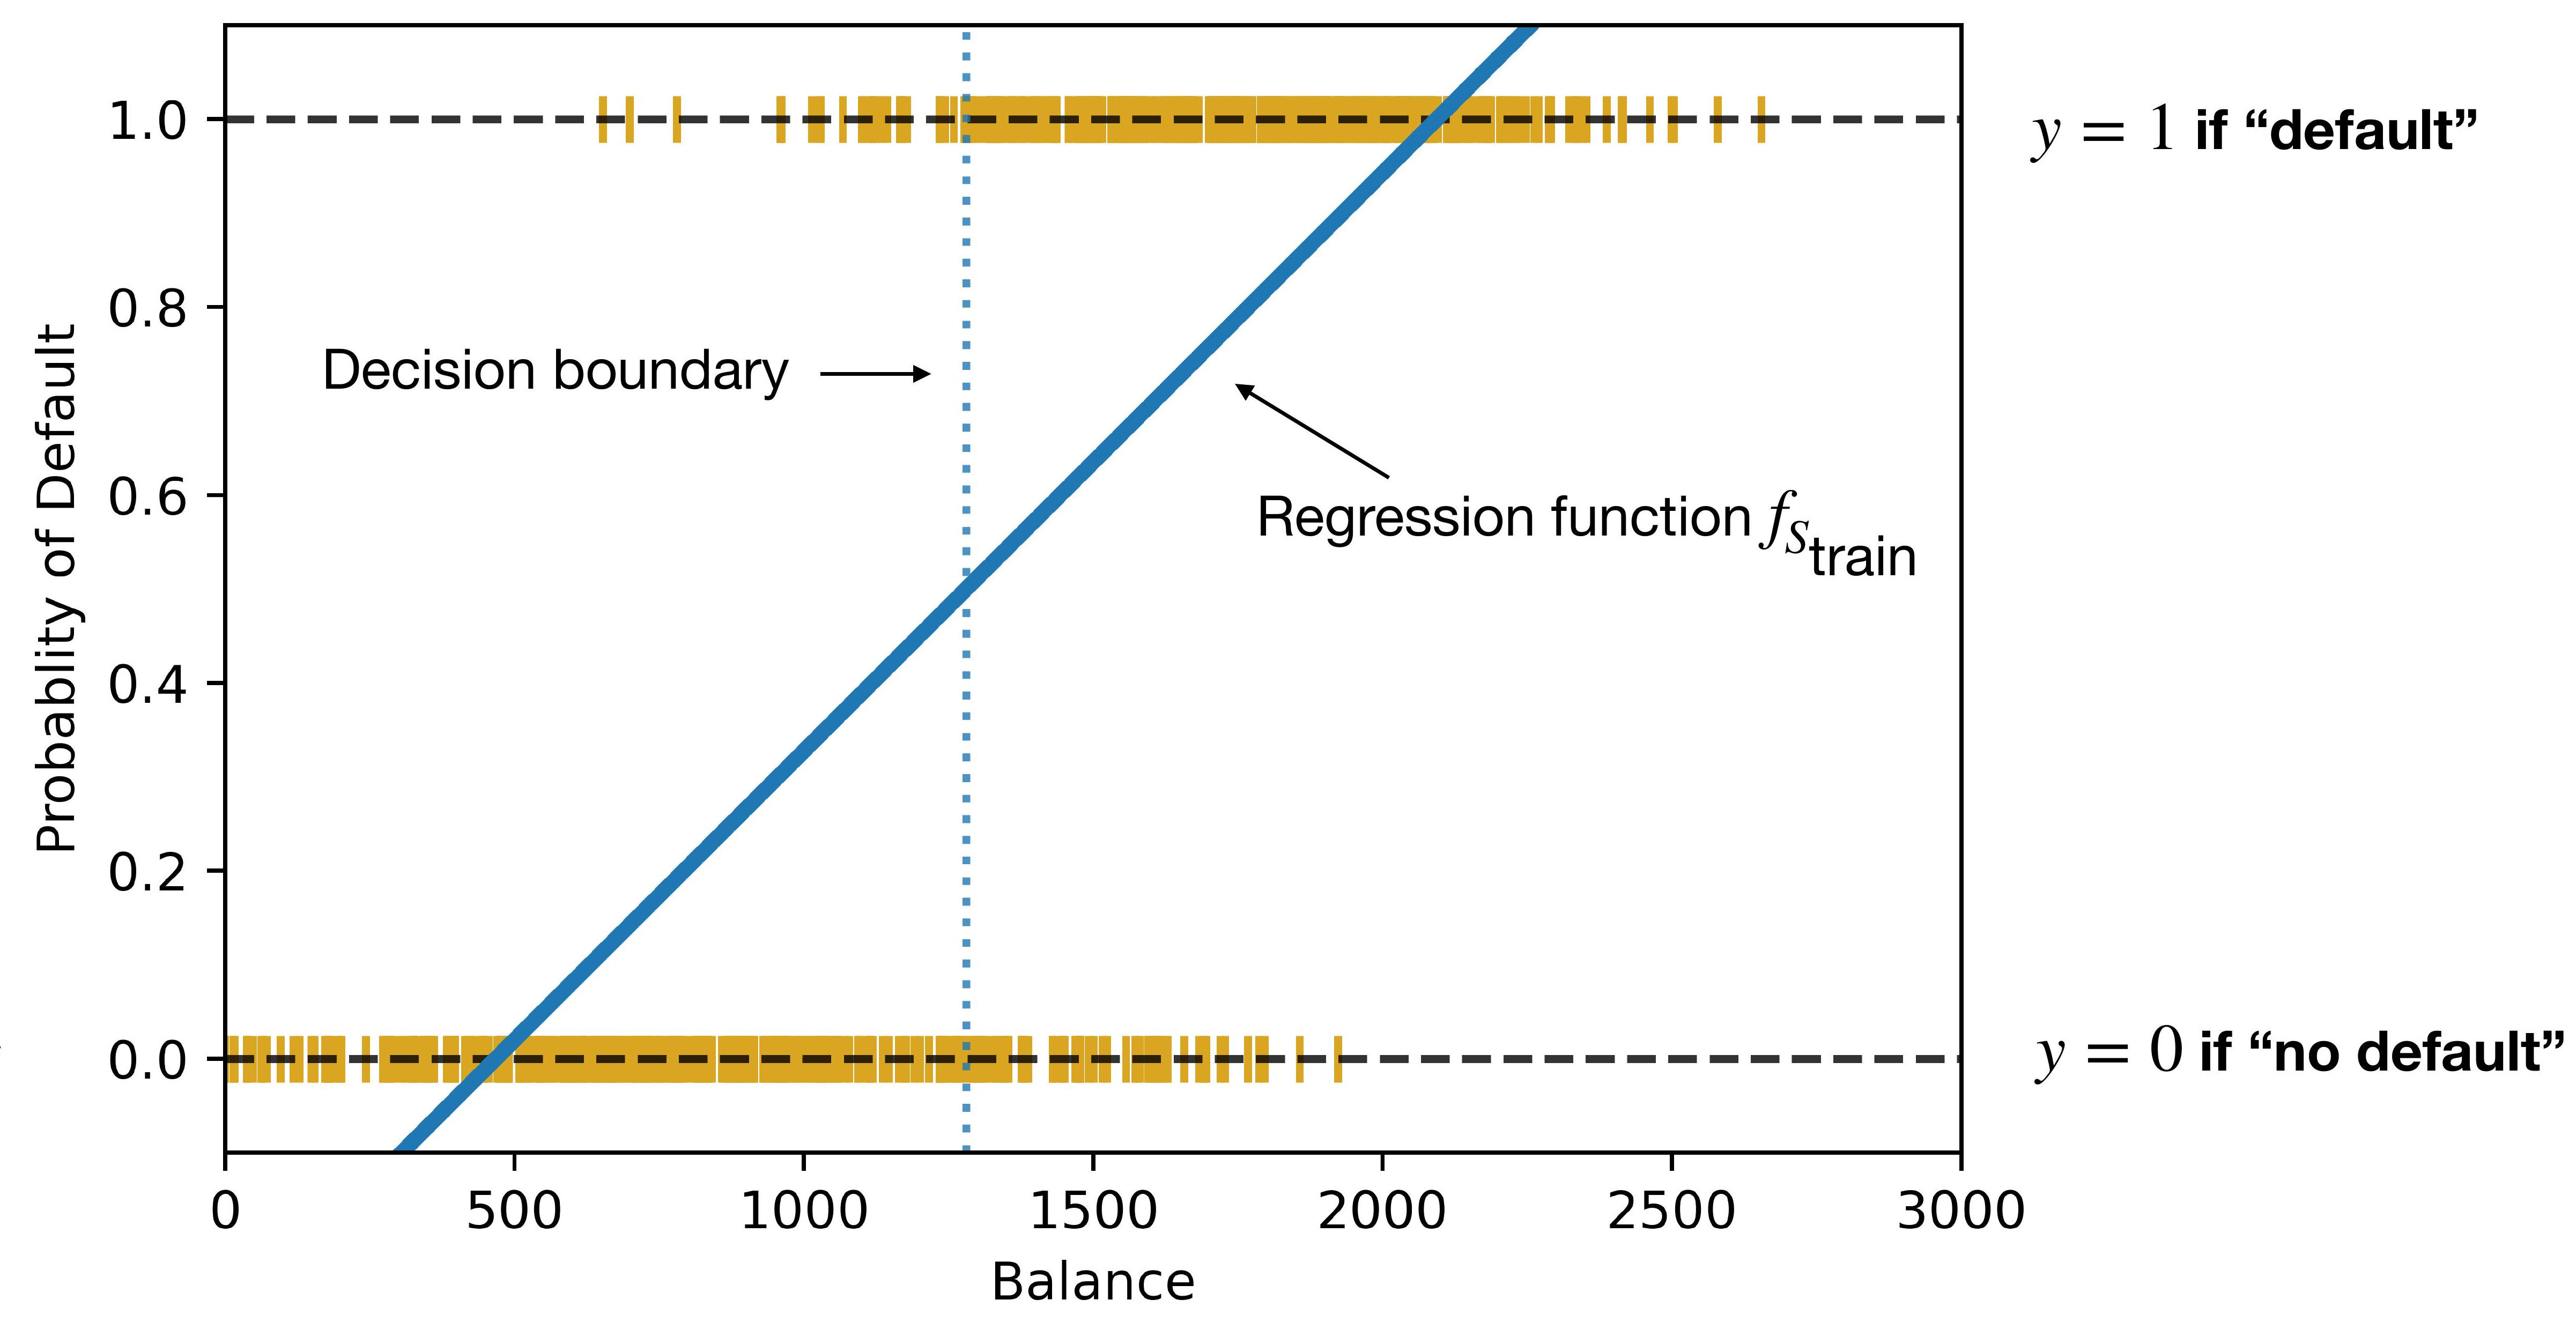
\includegraphics[max width=\textwidth]{2023_12_30_cf784c471dfd1dd5afbag-12}
\end{center}

\section*{Classification is not just a special form of regression}
A. The predicted values are not probabilities (not in $[0,1]$ )

\begin{center}
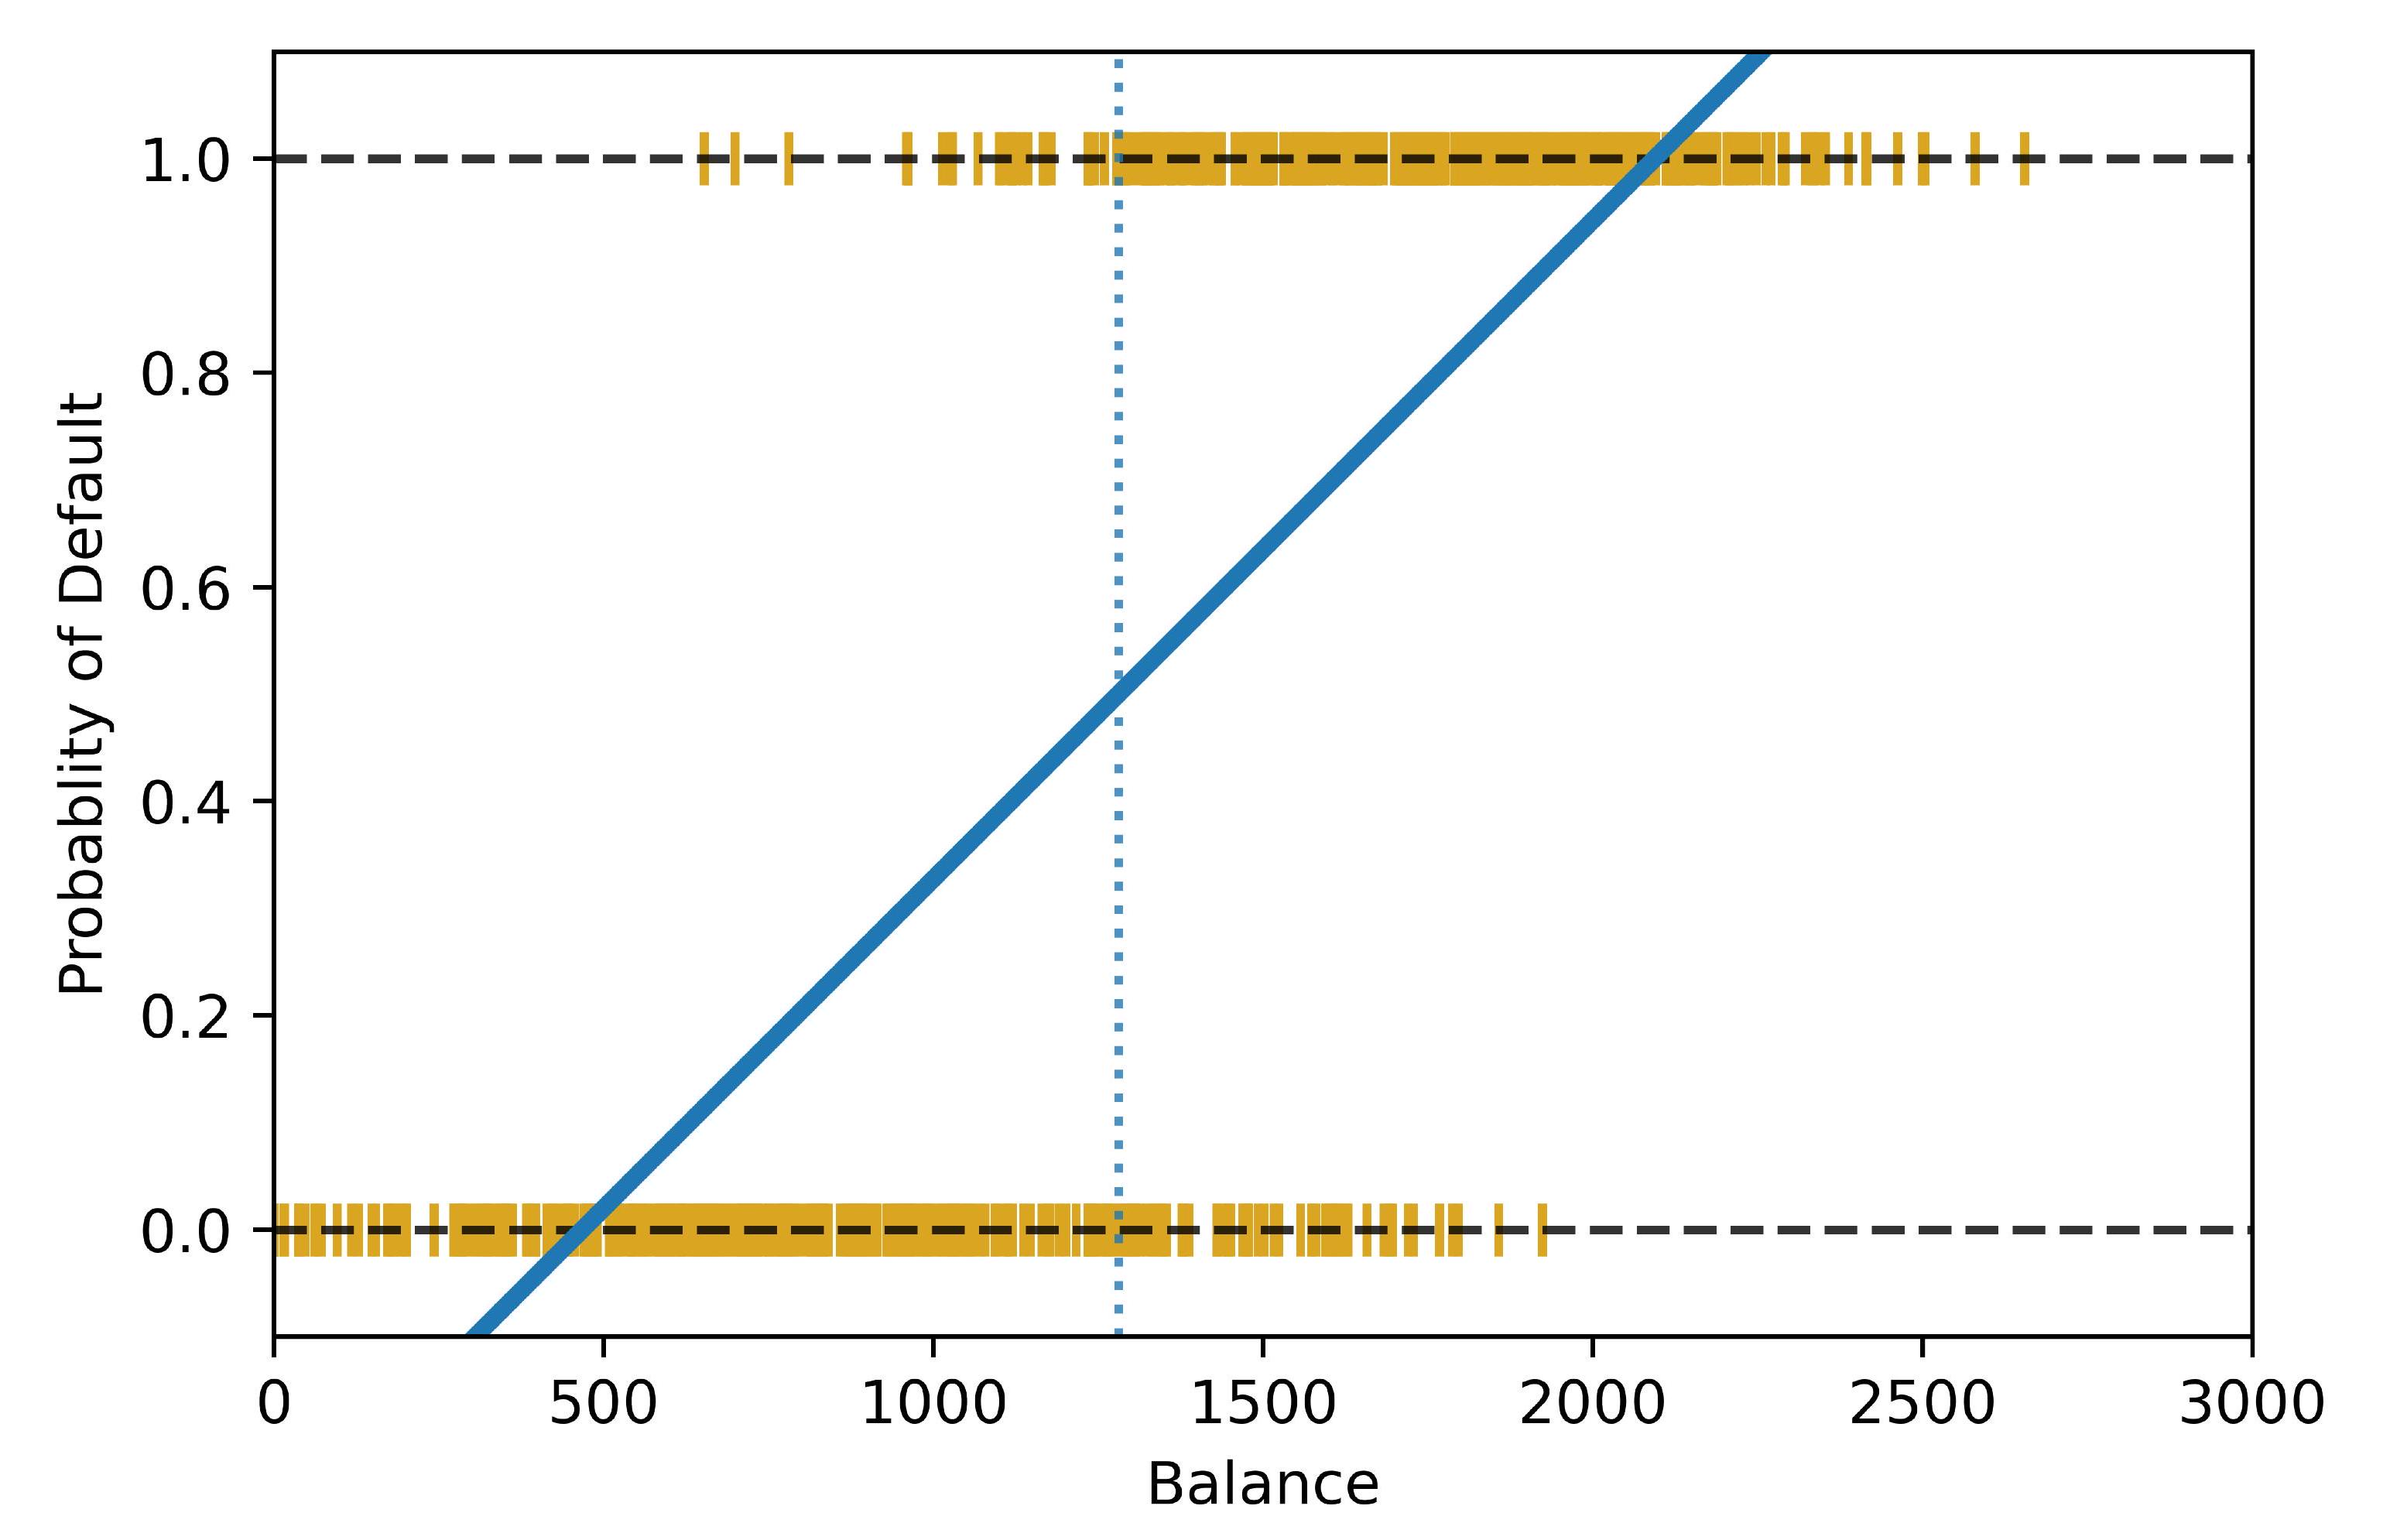
\includegraphics[max width=\textwidth]{2023_12_30_cf784c471dfd1dd5afbag-13}
\end{center}

\section*{Classification is not just a special form of regression}
B. Sensitivity to unbalanced data

\begin{center}
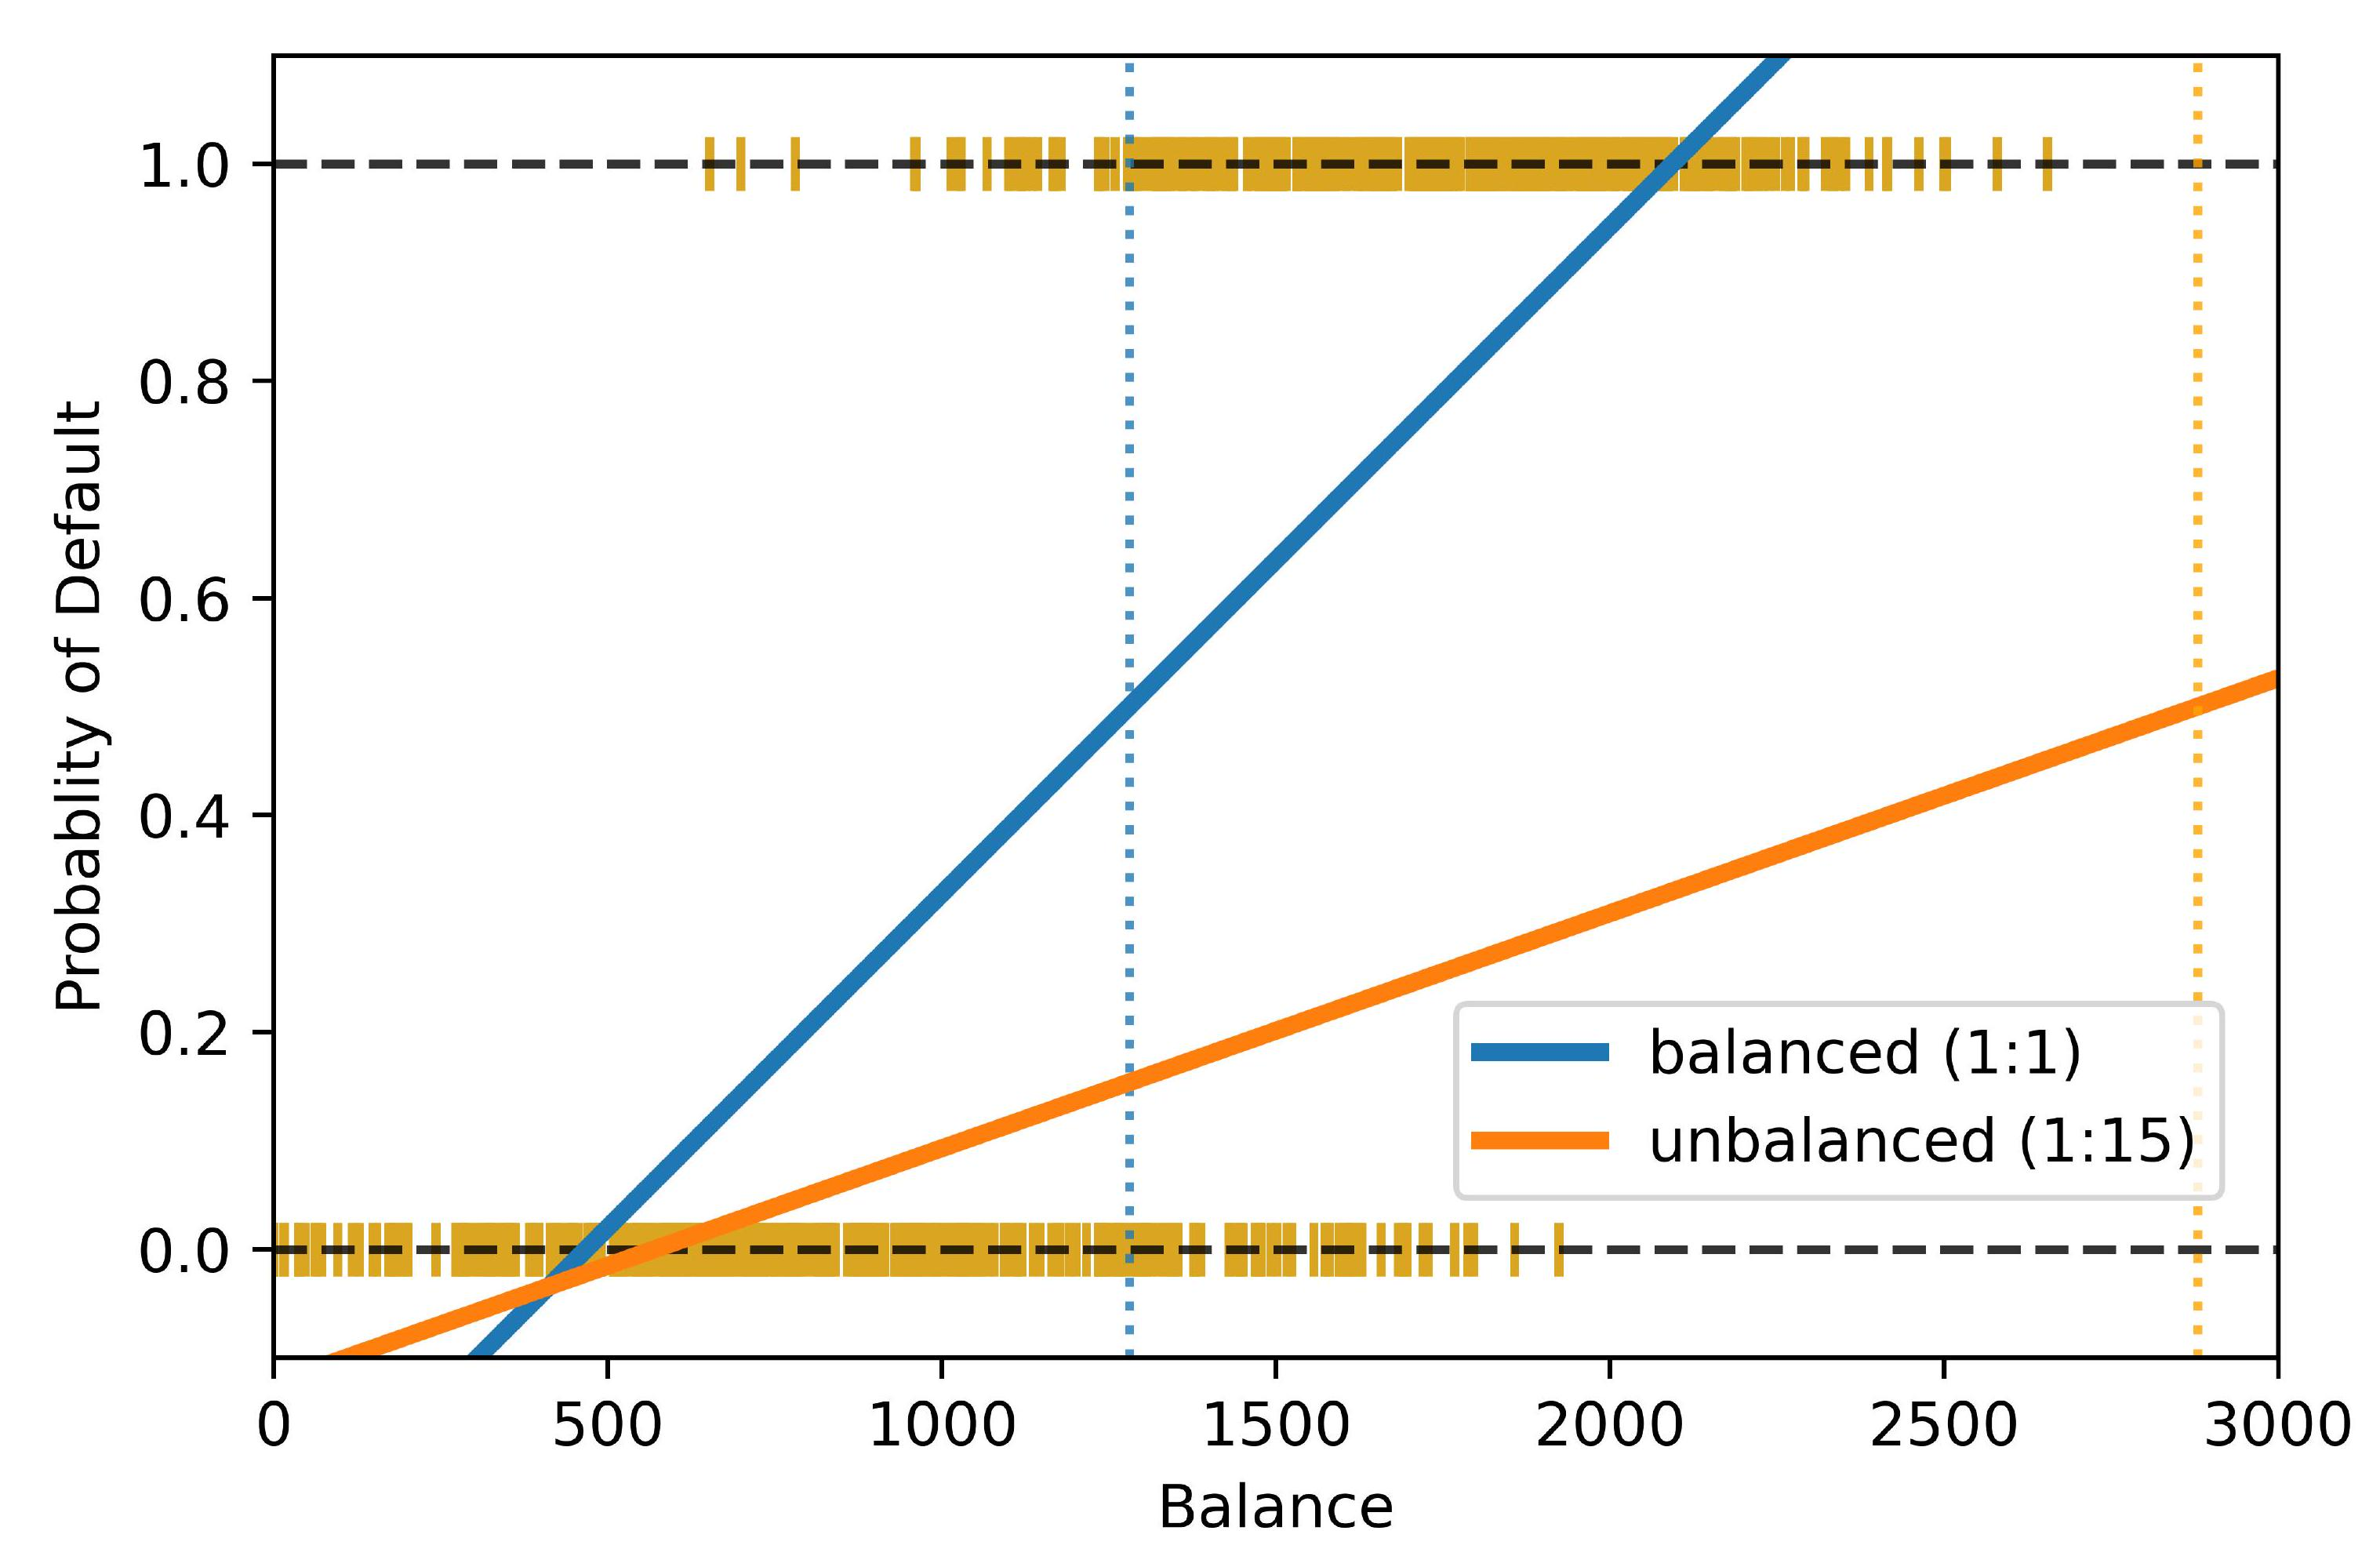
\includegraphics[max width=\textwidth]{2023_12_30_cf784c471dfd1dd5afbag-14}
\end{center}

The position of the line depends crucially on how many points are in each class

\section*{Classification is not just a special form of regression}
C. Sensitivity to extreme values:
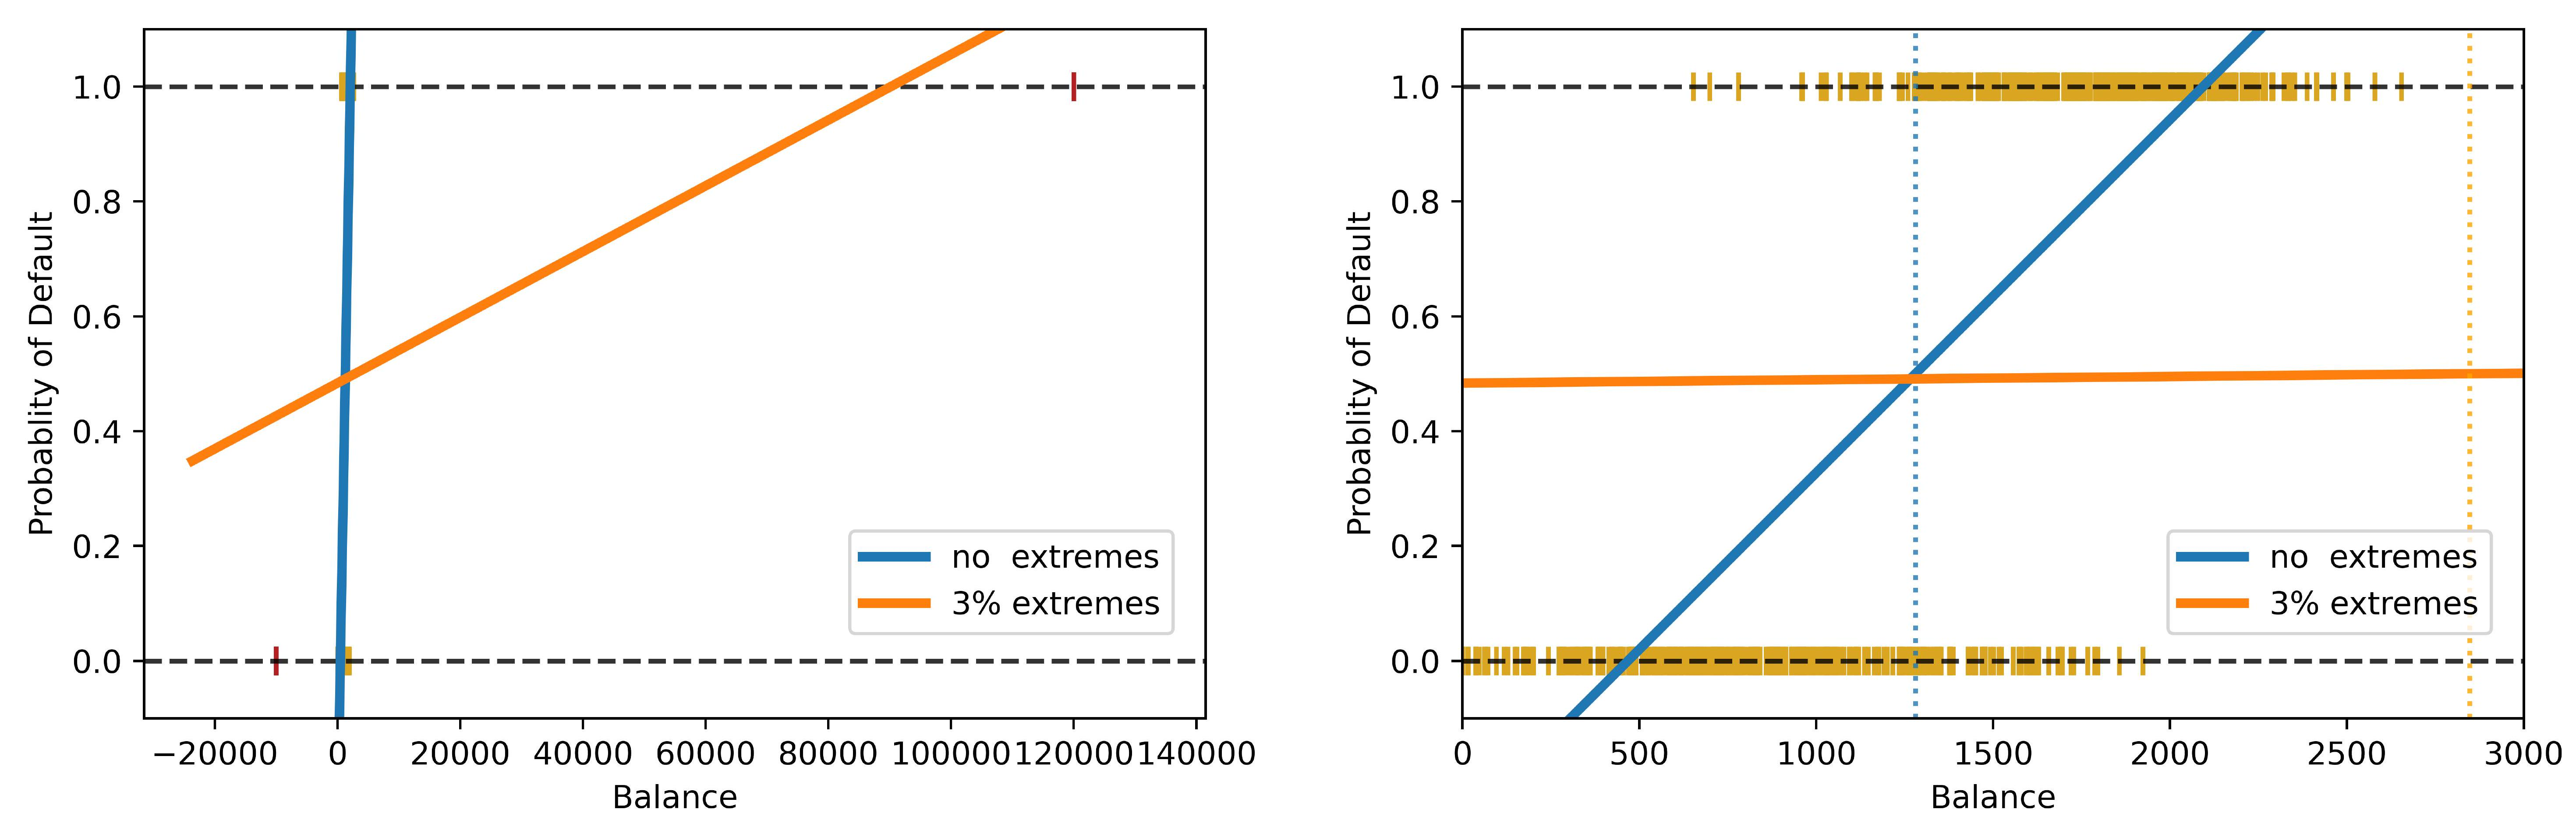
\includegraphics[max width=\textwidth, center]{2023_12_30_cf784c471dfd1dd5afbag-15}

The position of the line depends crucially on where the points lie

Why: the square loss we used for regression is not suitable for classification

\section*{How to perform classification?}
\begin{itemize}
  \item Many approaches have been developed

  \item We won't cover them in detail today

  \item Instead, we will provide quick introductions

  \item Fundamental task of classification:

\end{itemize}

\begin{center}
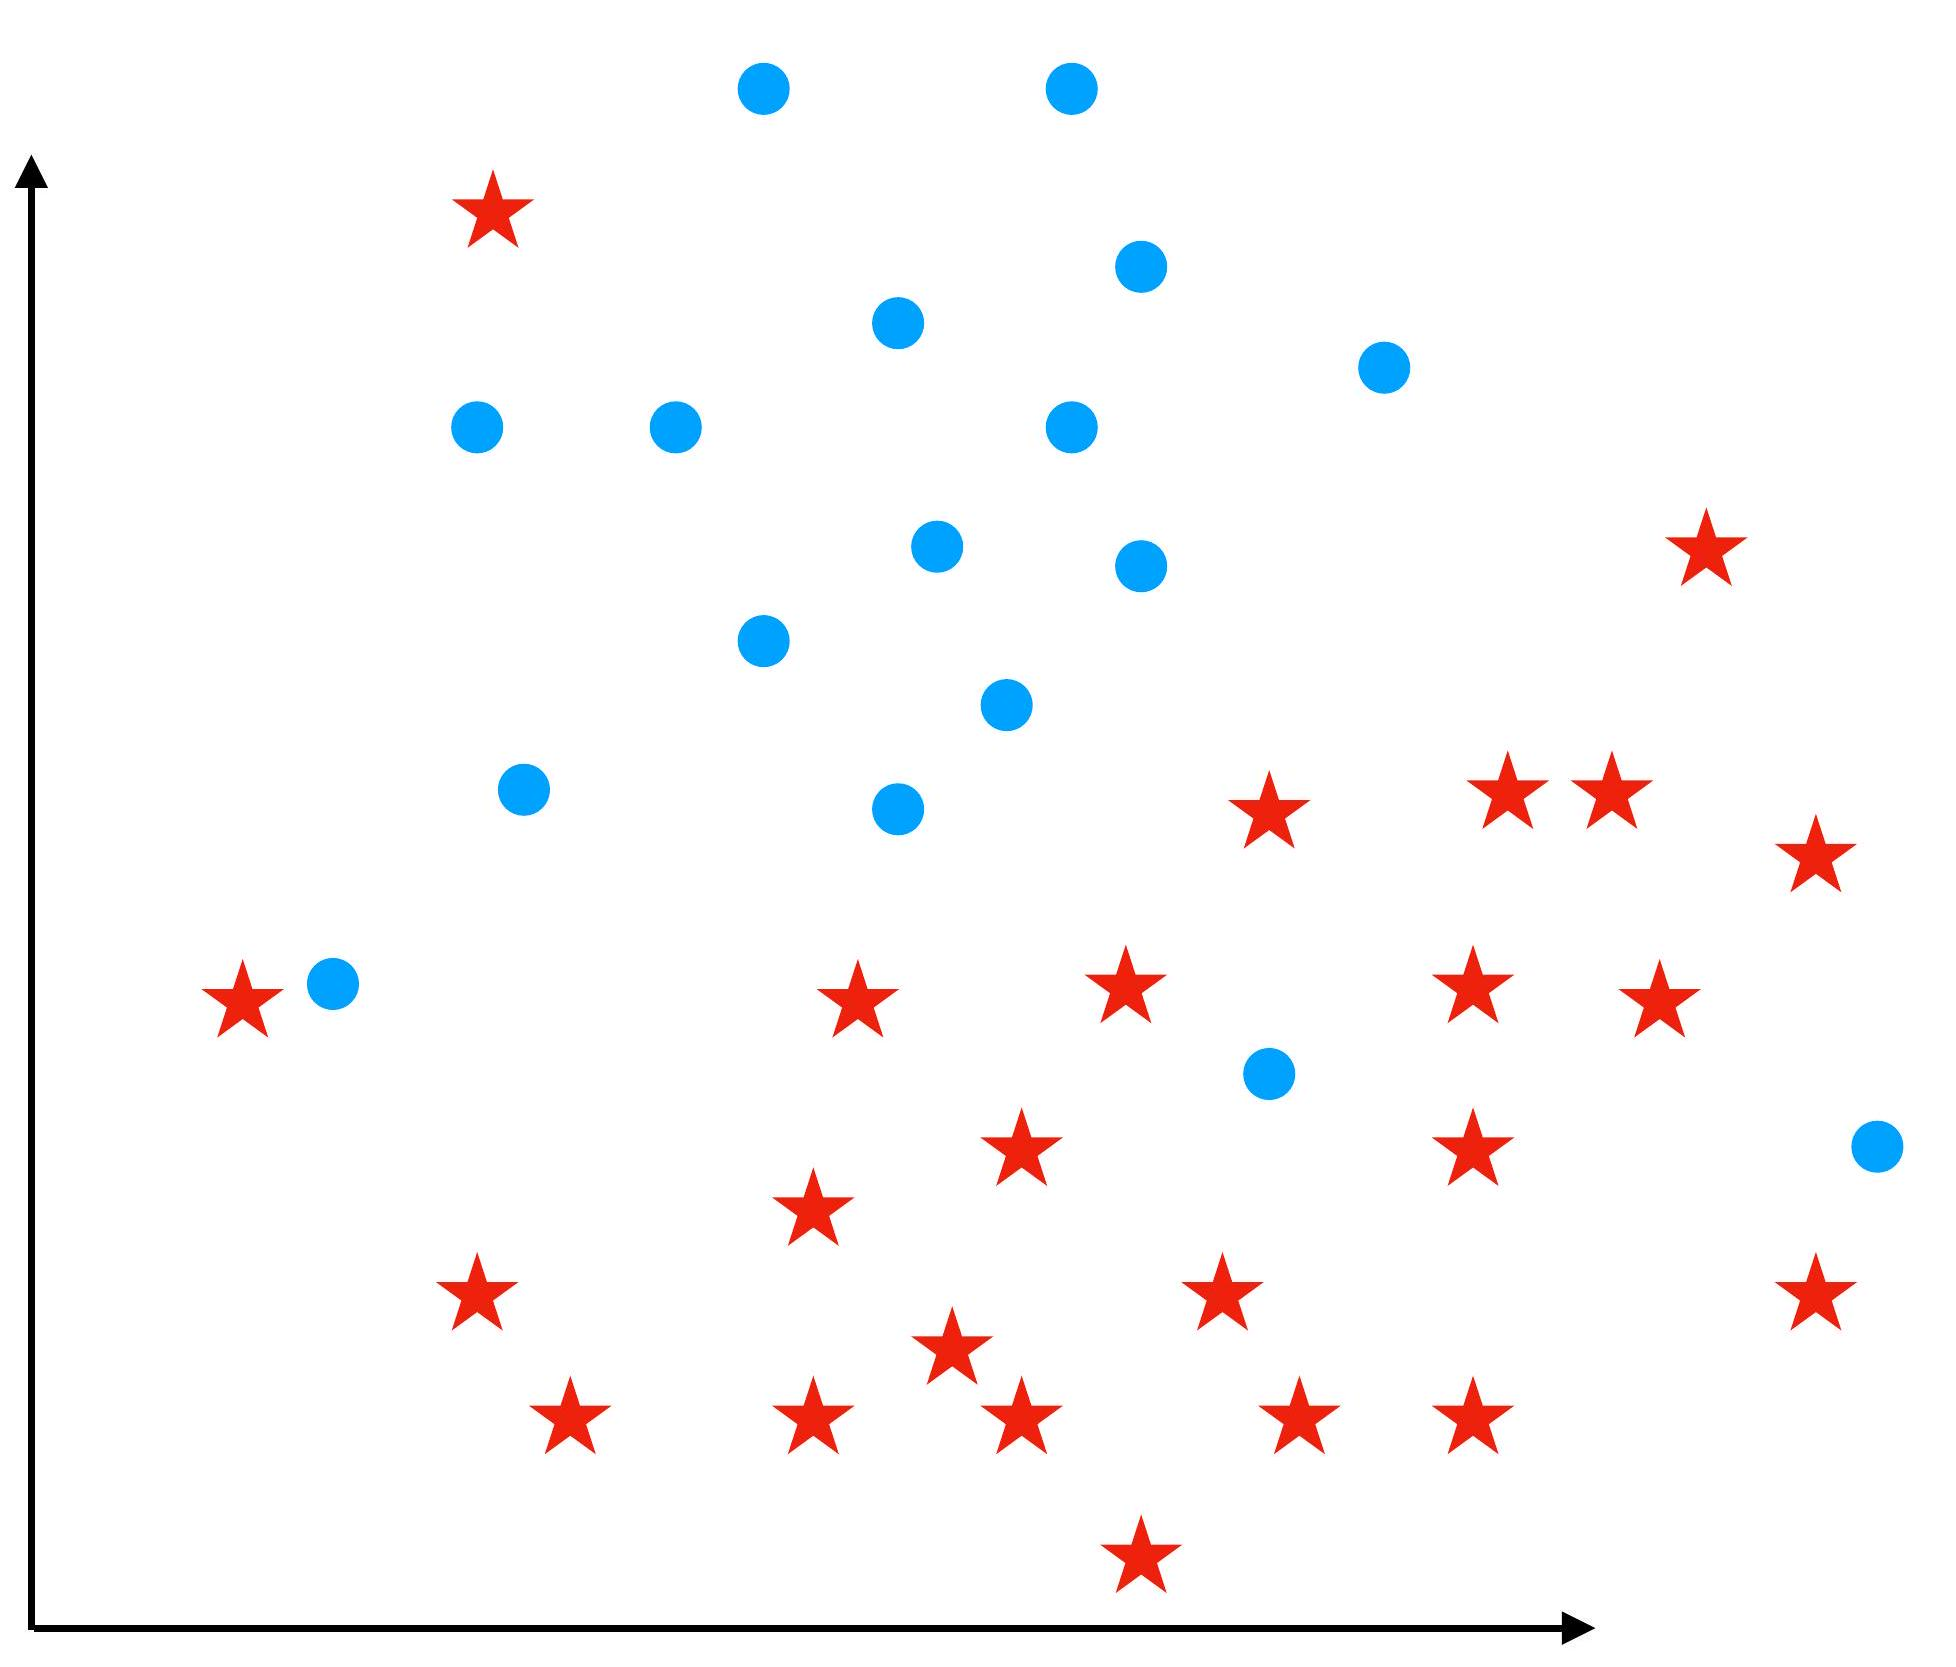
\includegraphics[max width=\textwidth]{2023_12_30_cf784c471dfd1dd5afbag-16}
\end{center}

Divide the space into distinct decision regions

\section*{k-Nearest Neighbor}
\begin{center}
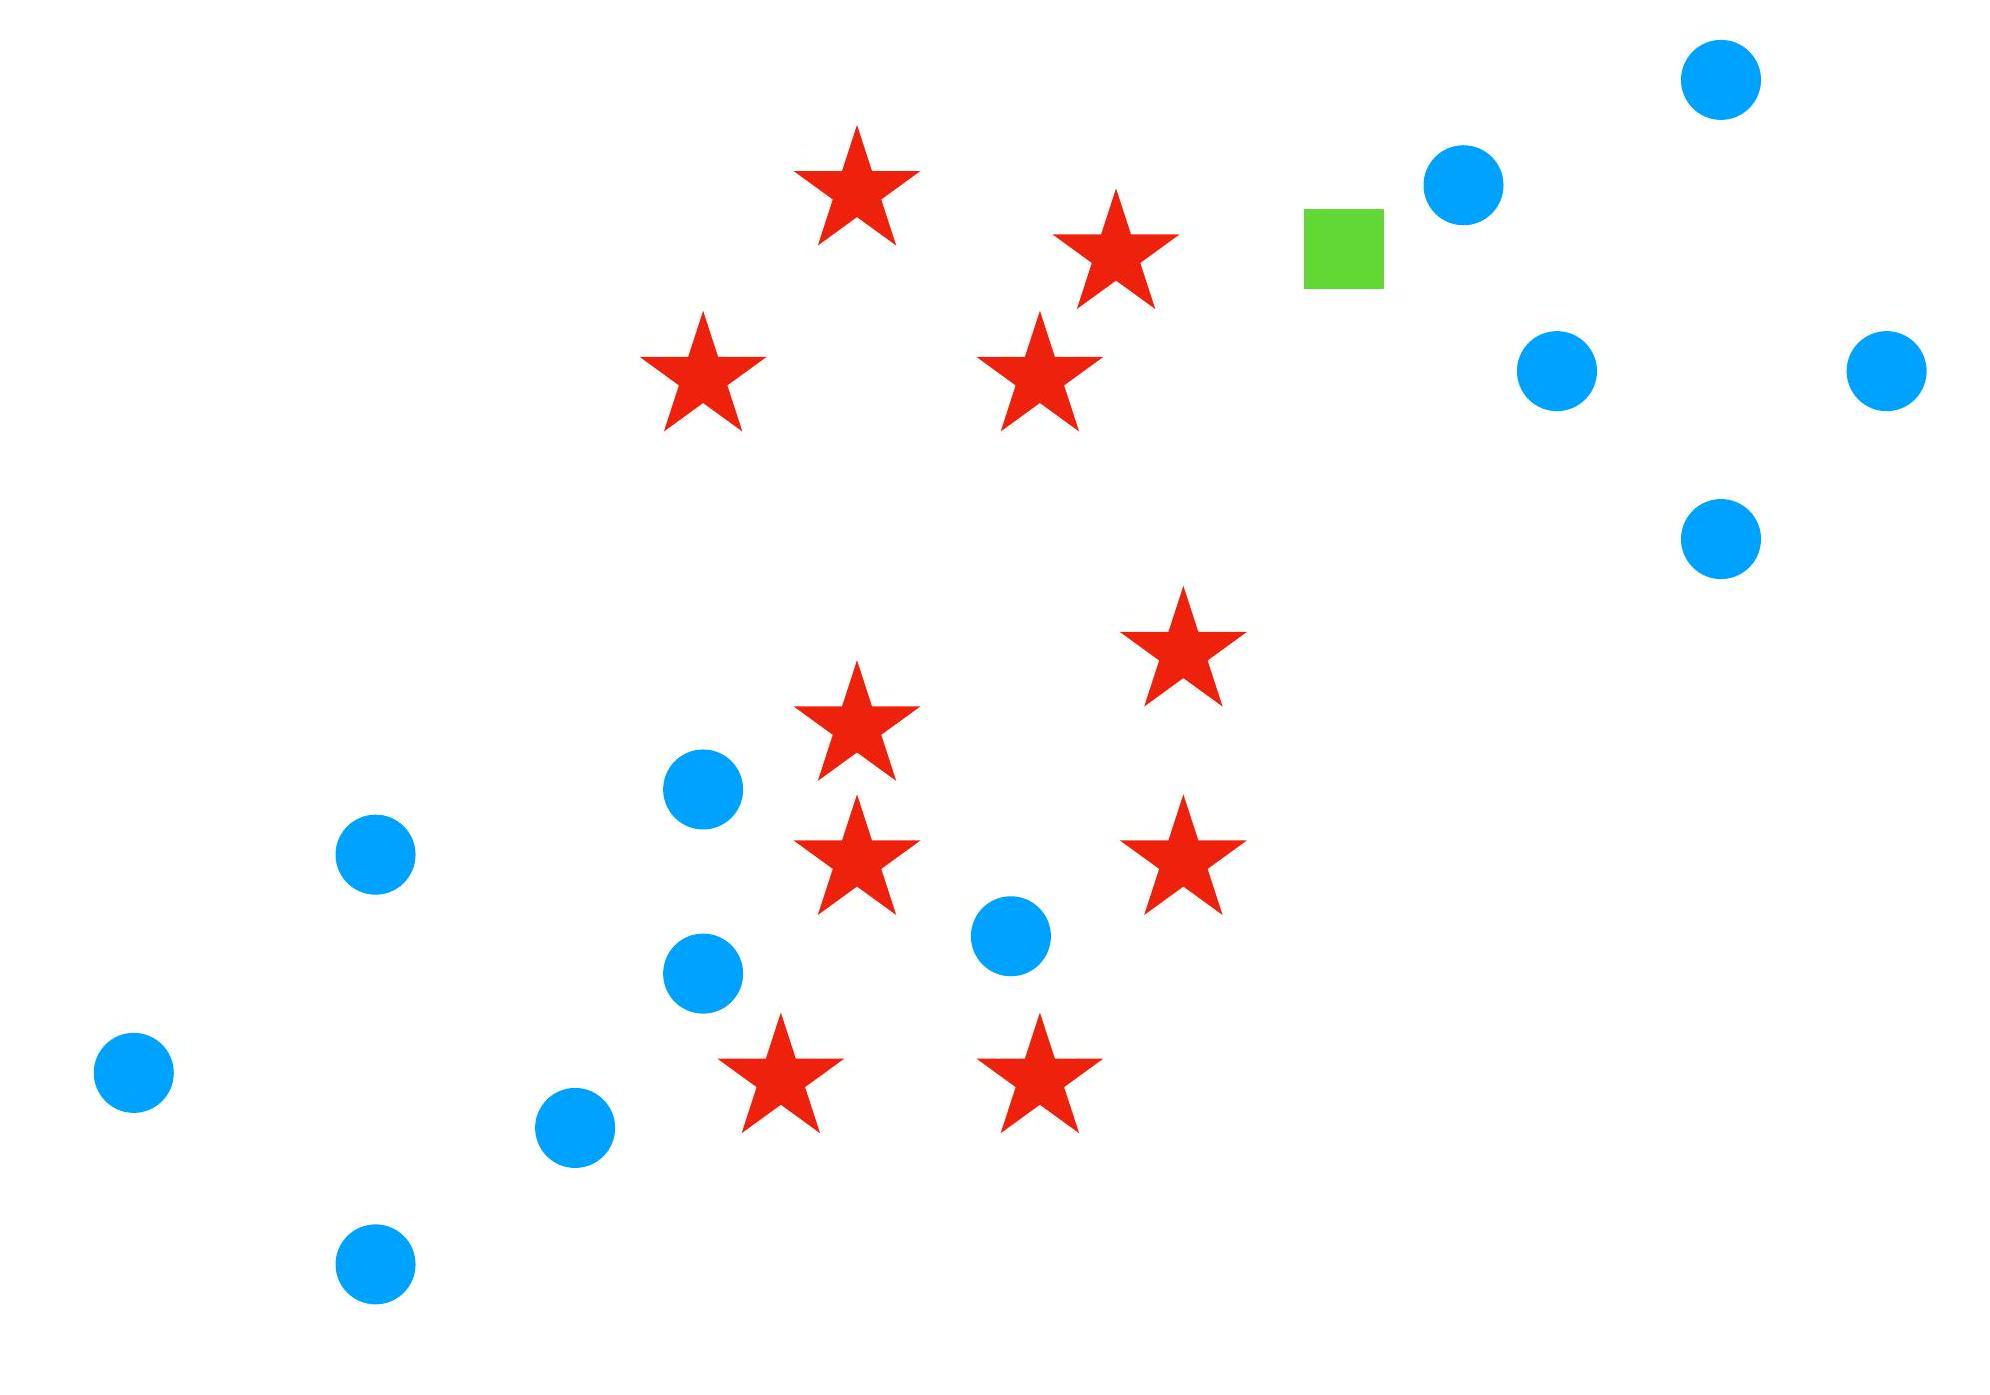
\includegraphics[max width=\textwidth]{2023_12_30_cf784c471dfd1dd5afbag-17}
\end{center}

\begin{center}
\begin{tabular}{|ll|}
\hline
 & Class 1 \\
$\star$ & Class 2 \\
 & Testing point \\
\hline
\end{tabular}
\end{center}

\section*{k-Nearest Neighbor}
Assume that nearby points are likely to have similar labels

\begin{center}
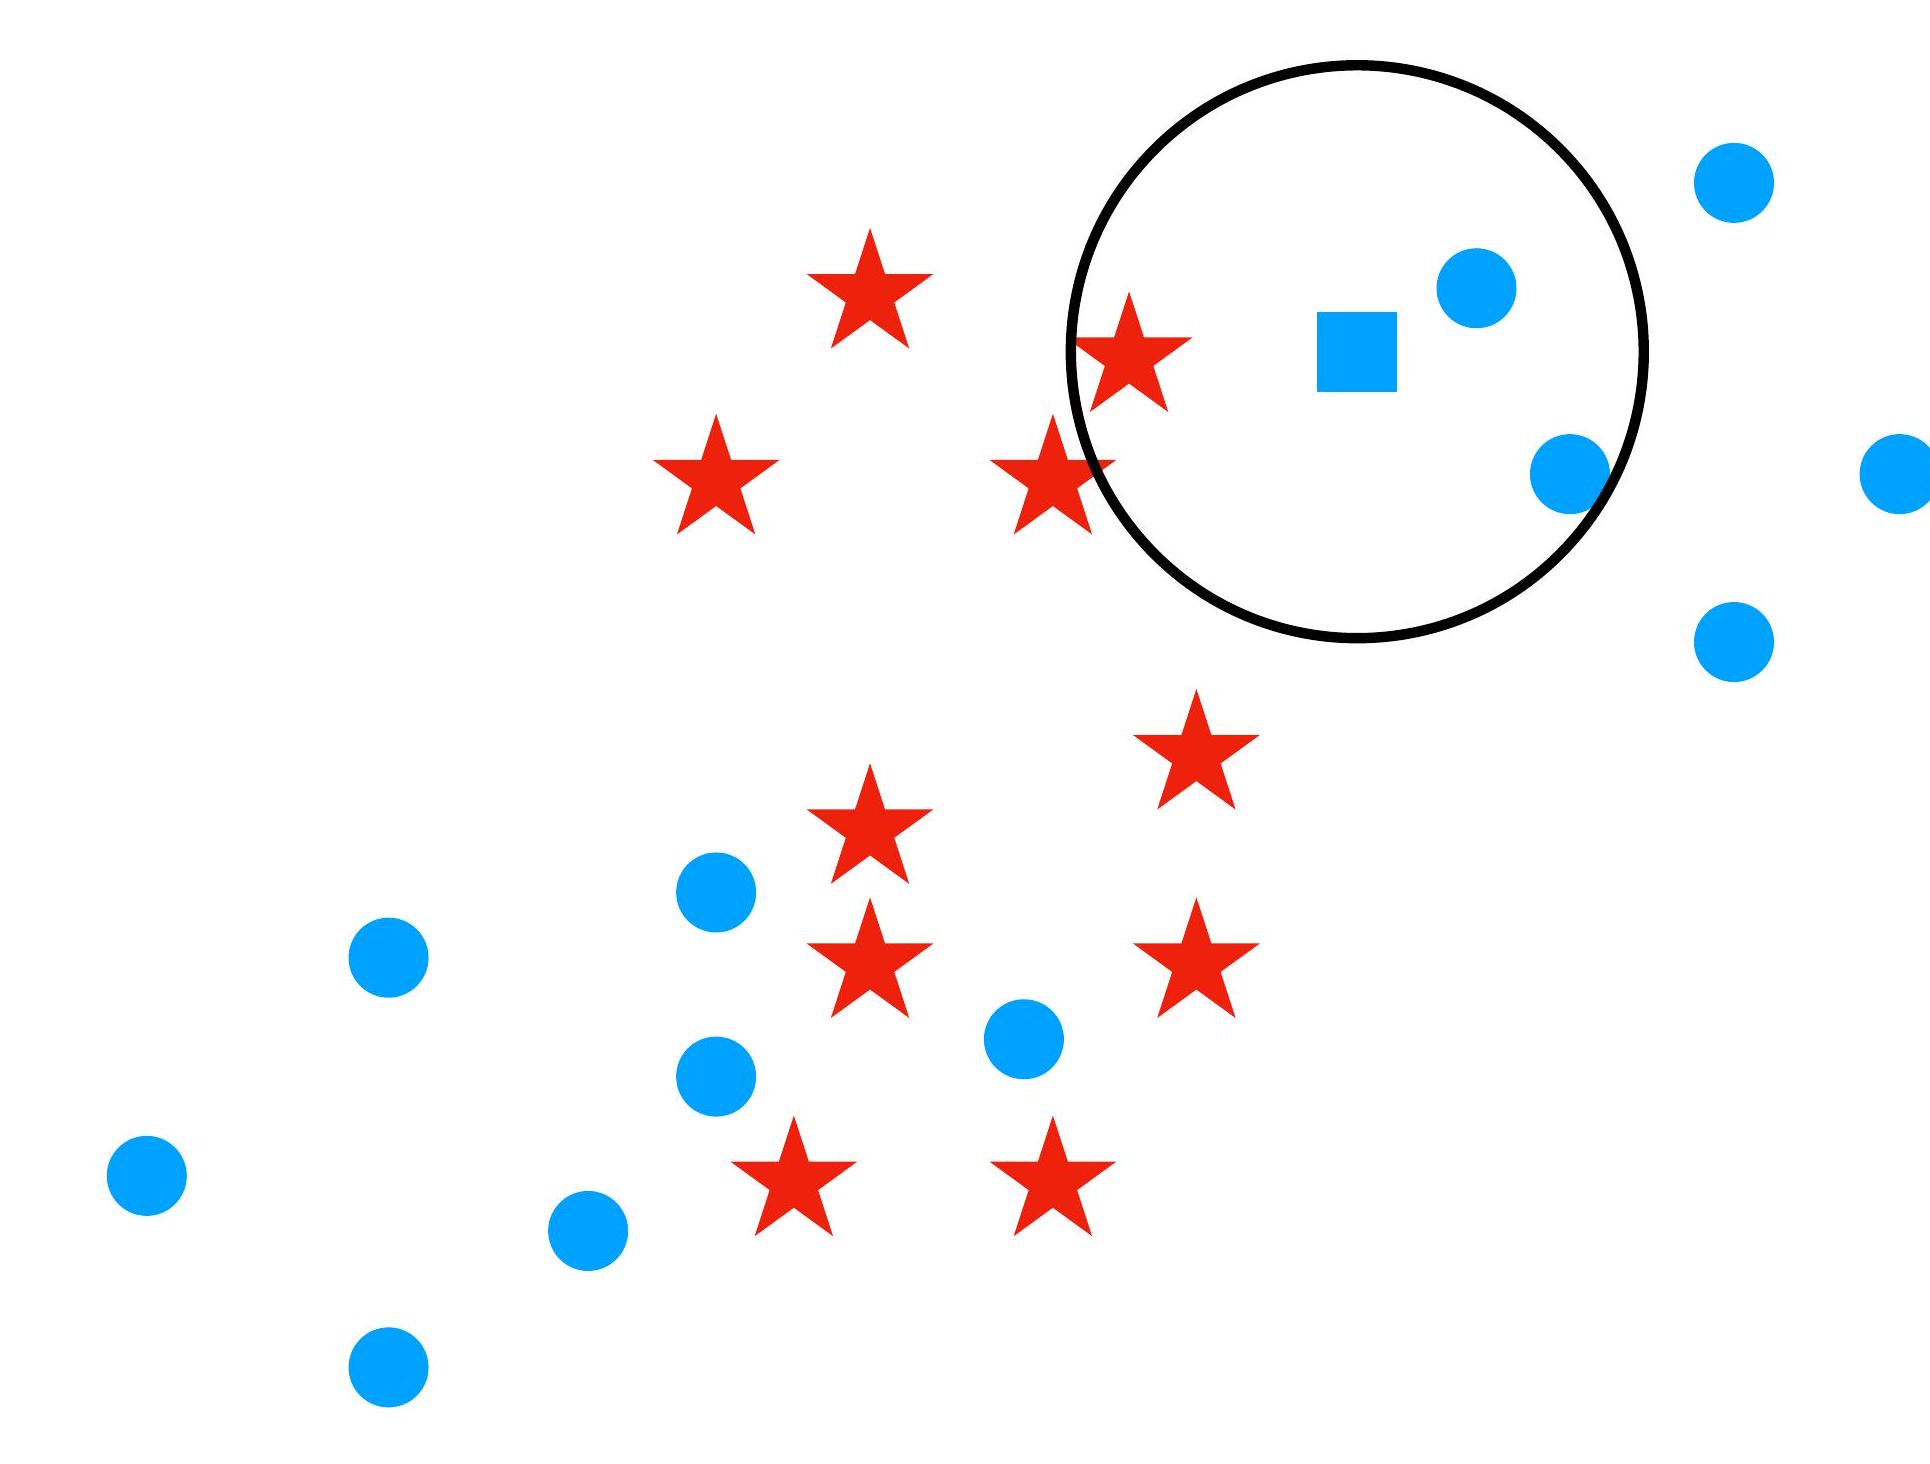
\includegraphics[max width=\textwidth]{2023_12_30_cf784c471dfd1dd5afbag-18}
\end{center}

\begin{center}
\begin{tabular}{|ll|}
\hline
 & Class 1 \\
$\star$ & Class 2 \\
 & Testing point \\
\hline
\end{tabular}
\end{center}

A new point $x$ is classified based on the majority vote of its $\mathbf{k}$-nearest neighbors

\section*{k-Nearest Neighbor}
Pros:

\begin{itemize}
  \item No optimization or training
  \item Easy to implement
  \item Works well in low dimensions, allowing for very complex decision boundaries
\end{itemize}

Cons:

\begin{itemize}
  \item Slow at query time
  \item Not suitable for high-dimensional data
  \item Choosing the right local distance is crucial
\end{itemize}

\begin{center}
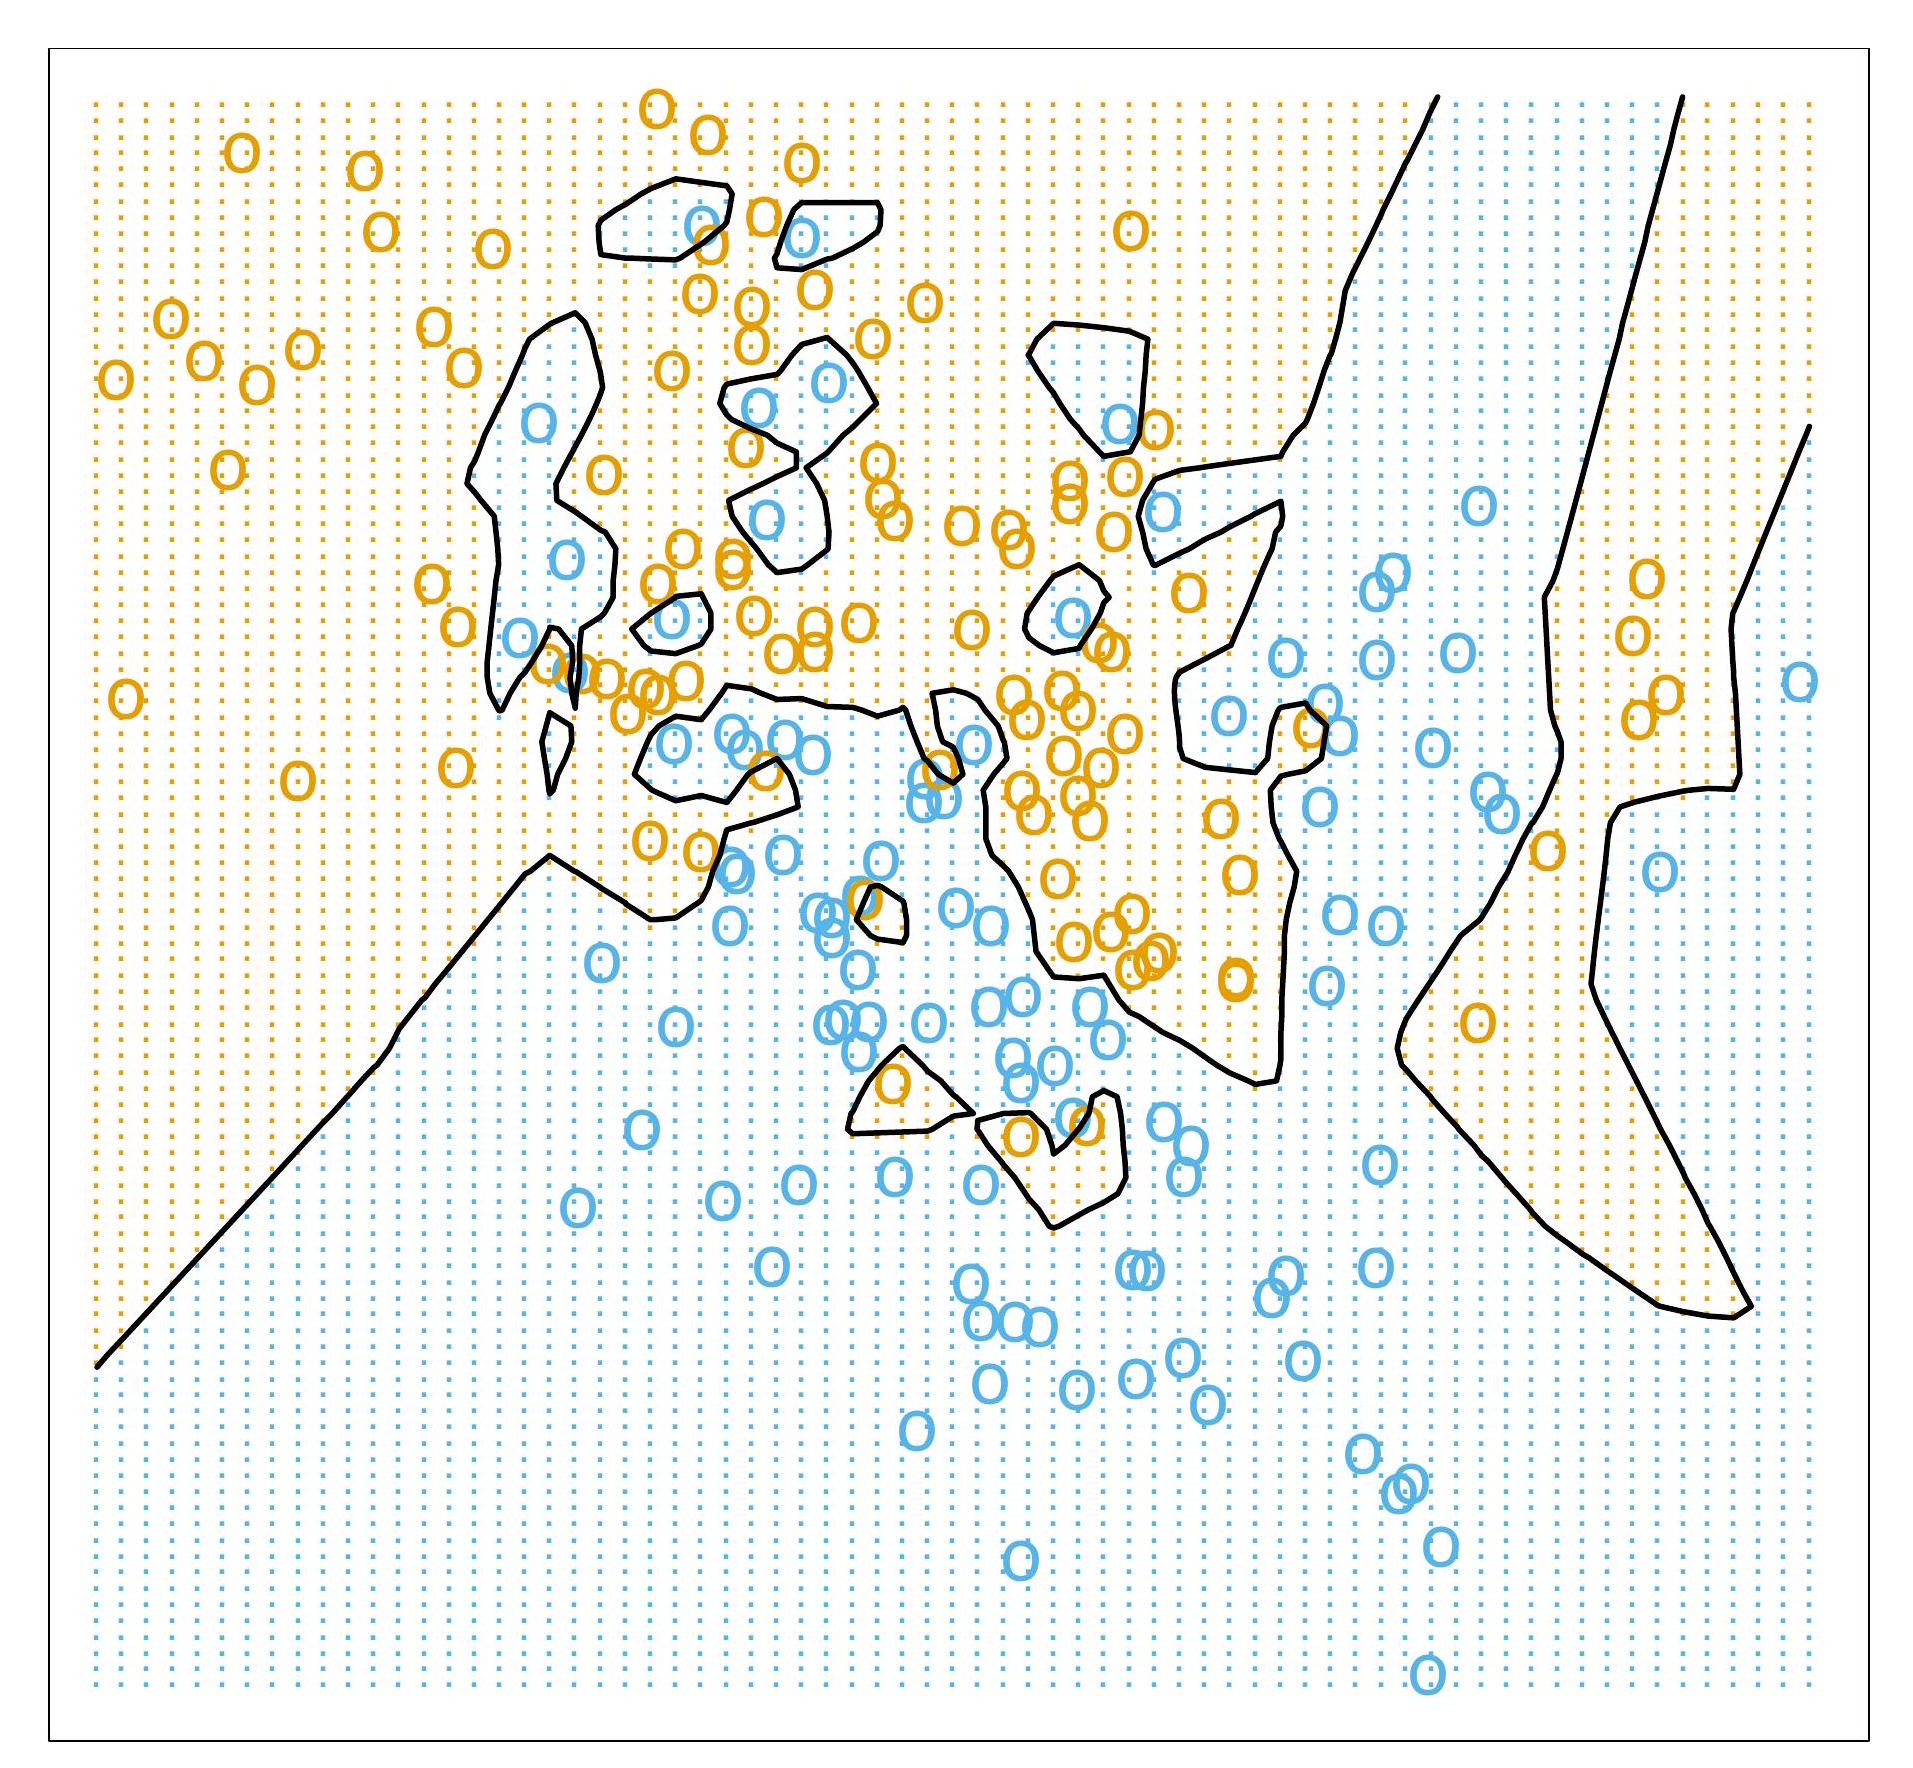
\includegraphics[max width=\textwidth]{2023_12_30_cf784c471dfd1dd5afbag-19}
\end{center}

\section*{Linear Decision boundaries}
Assume we restrict ourselves to linear decision boundaries (hyperplane):

$\Rightarrow$ Prediction: $f(x)=\operatorname{sign}\left(x^{\top} w\right)$

\begin{center}
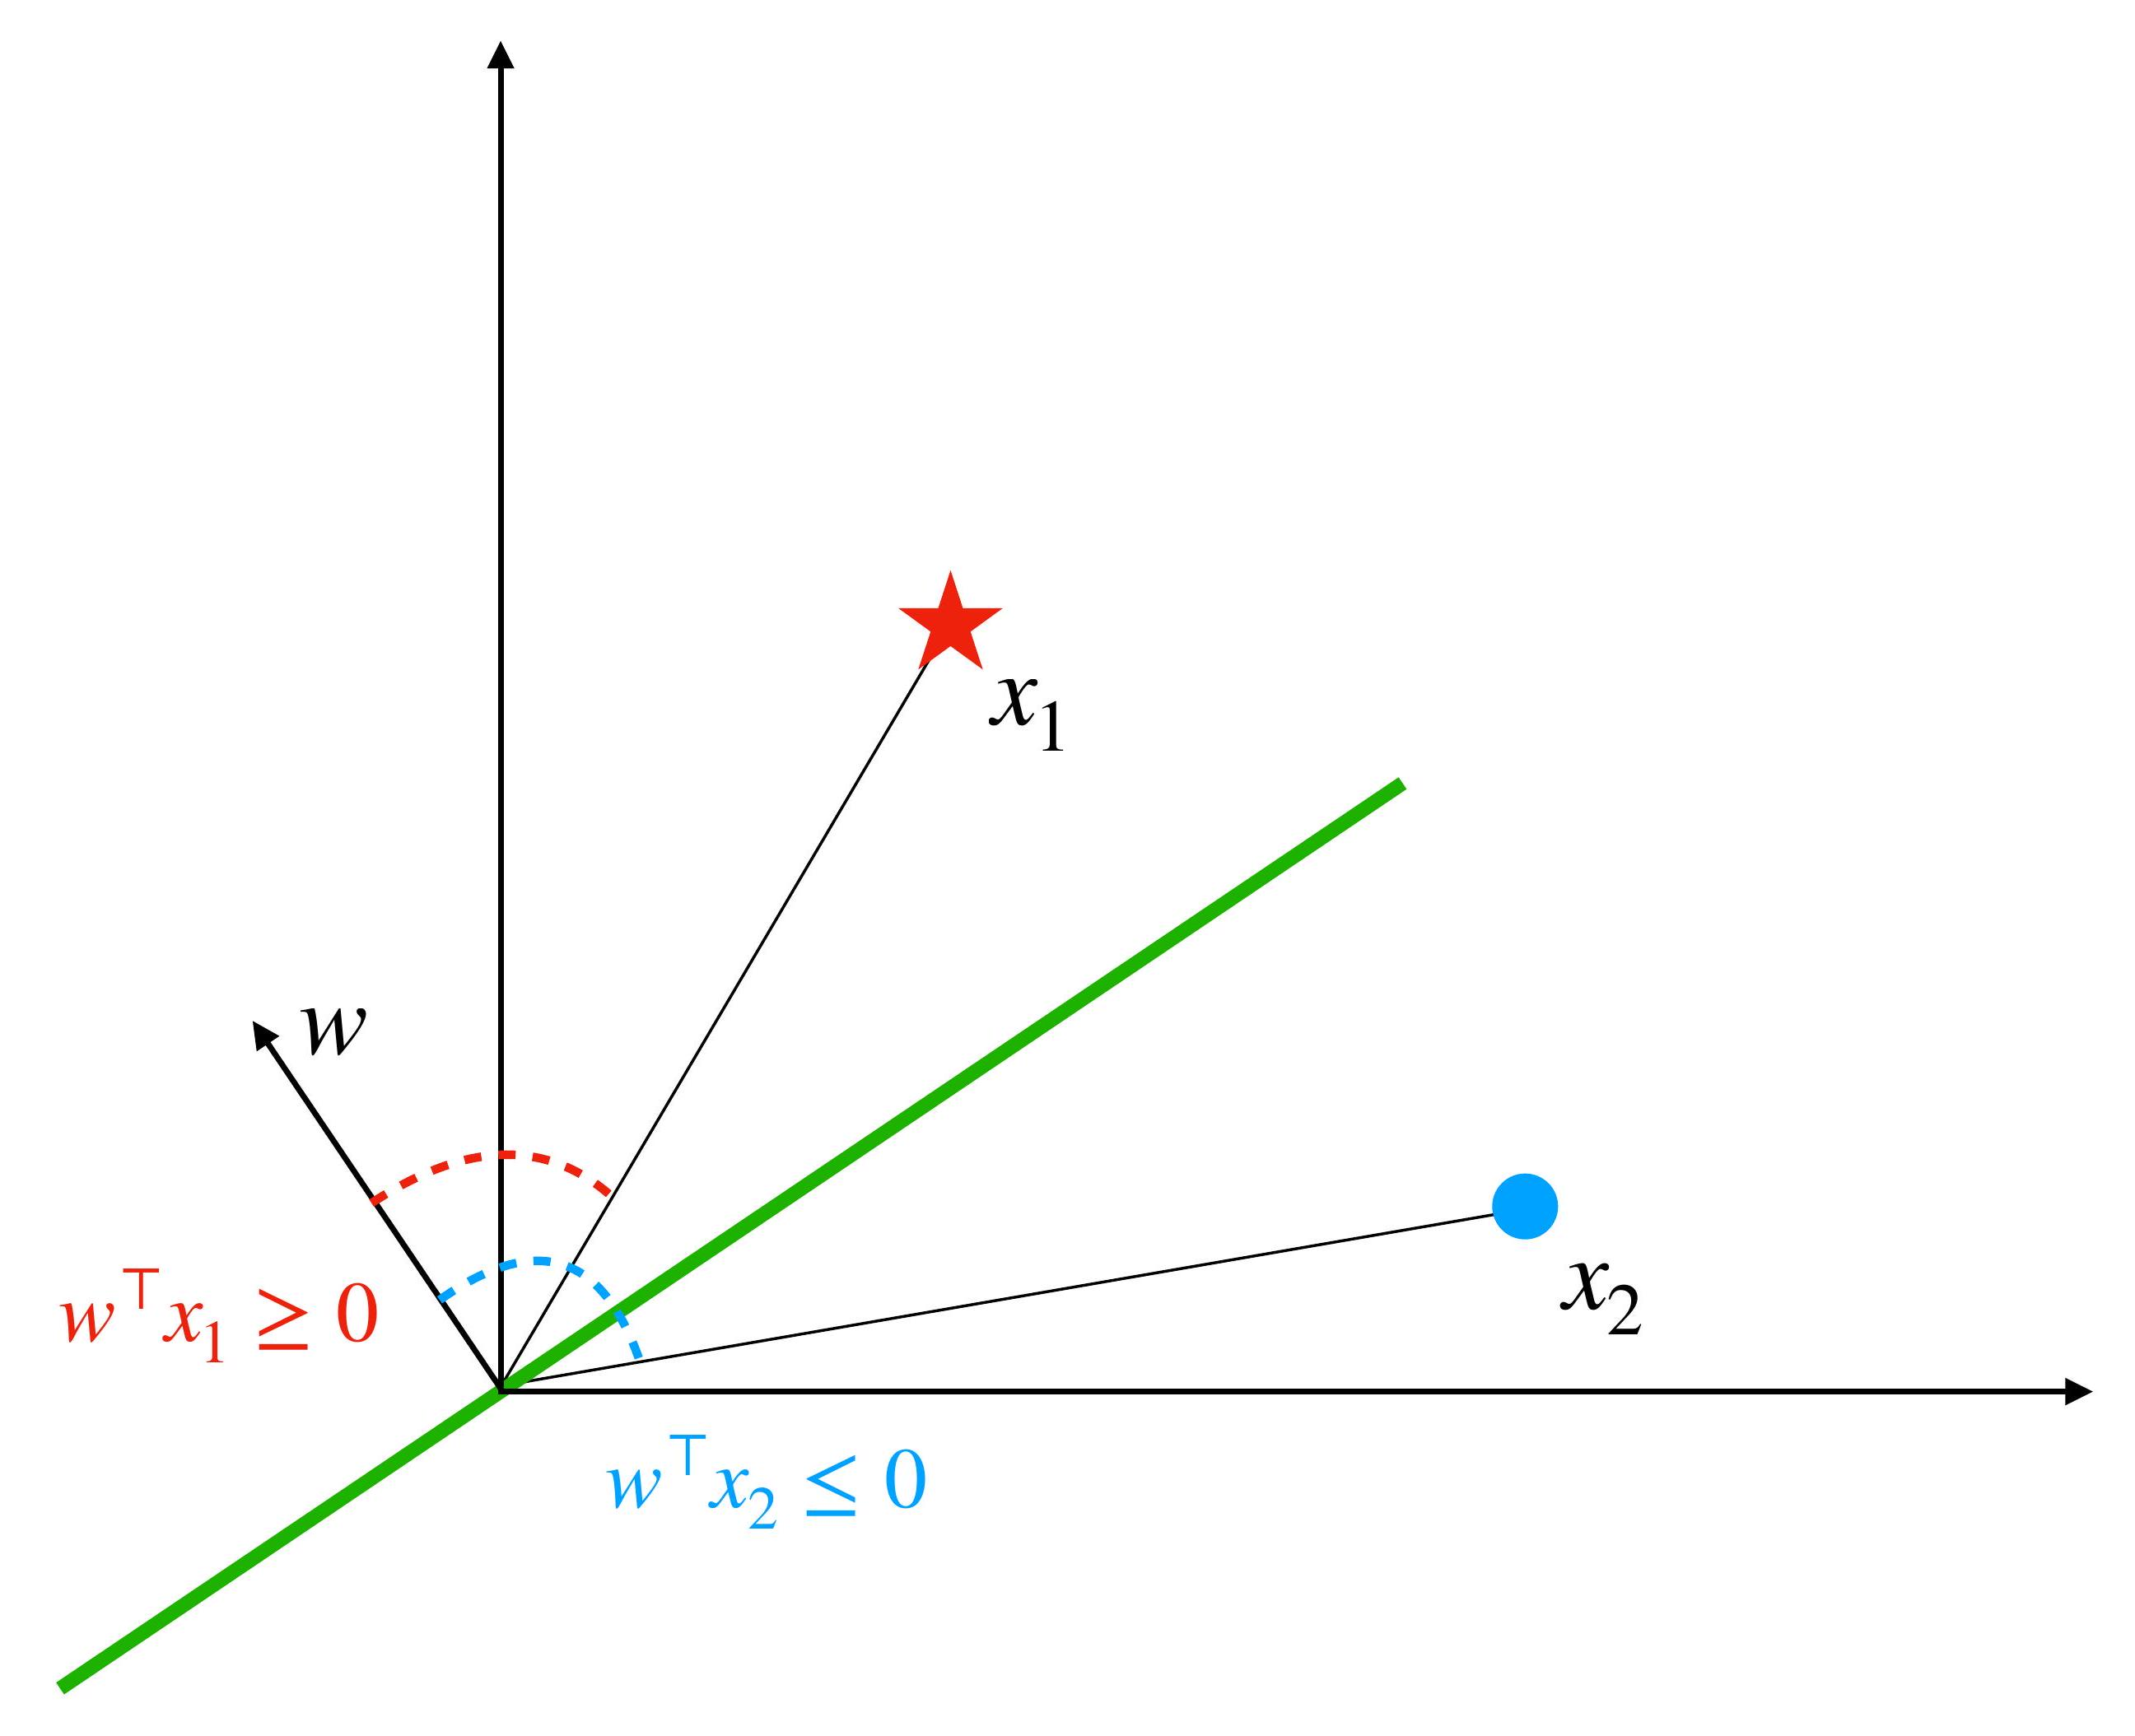
\includegraphics[max width=\textwidth]{2023_12_30_cf784c471dfd1dd5afbag-20}
\end{center}

\section*{Separating hyperplane}
Assume we restrict ourselves to linear decision boundaries (hyperplane): Assume the data are linearly separable, i.e., a separating hyperplane exists

\begin{center}
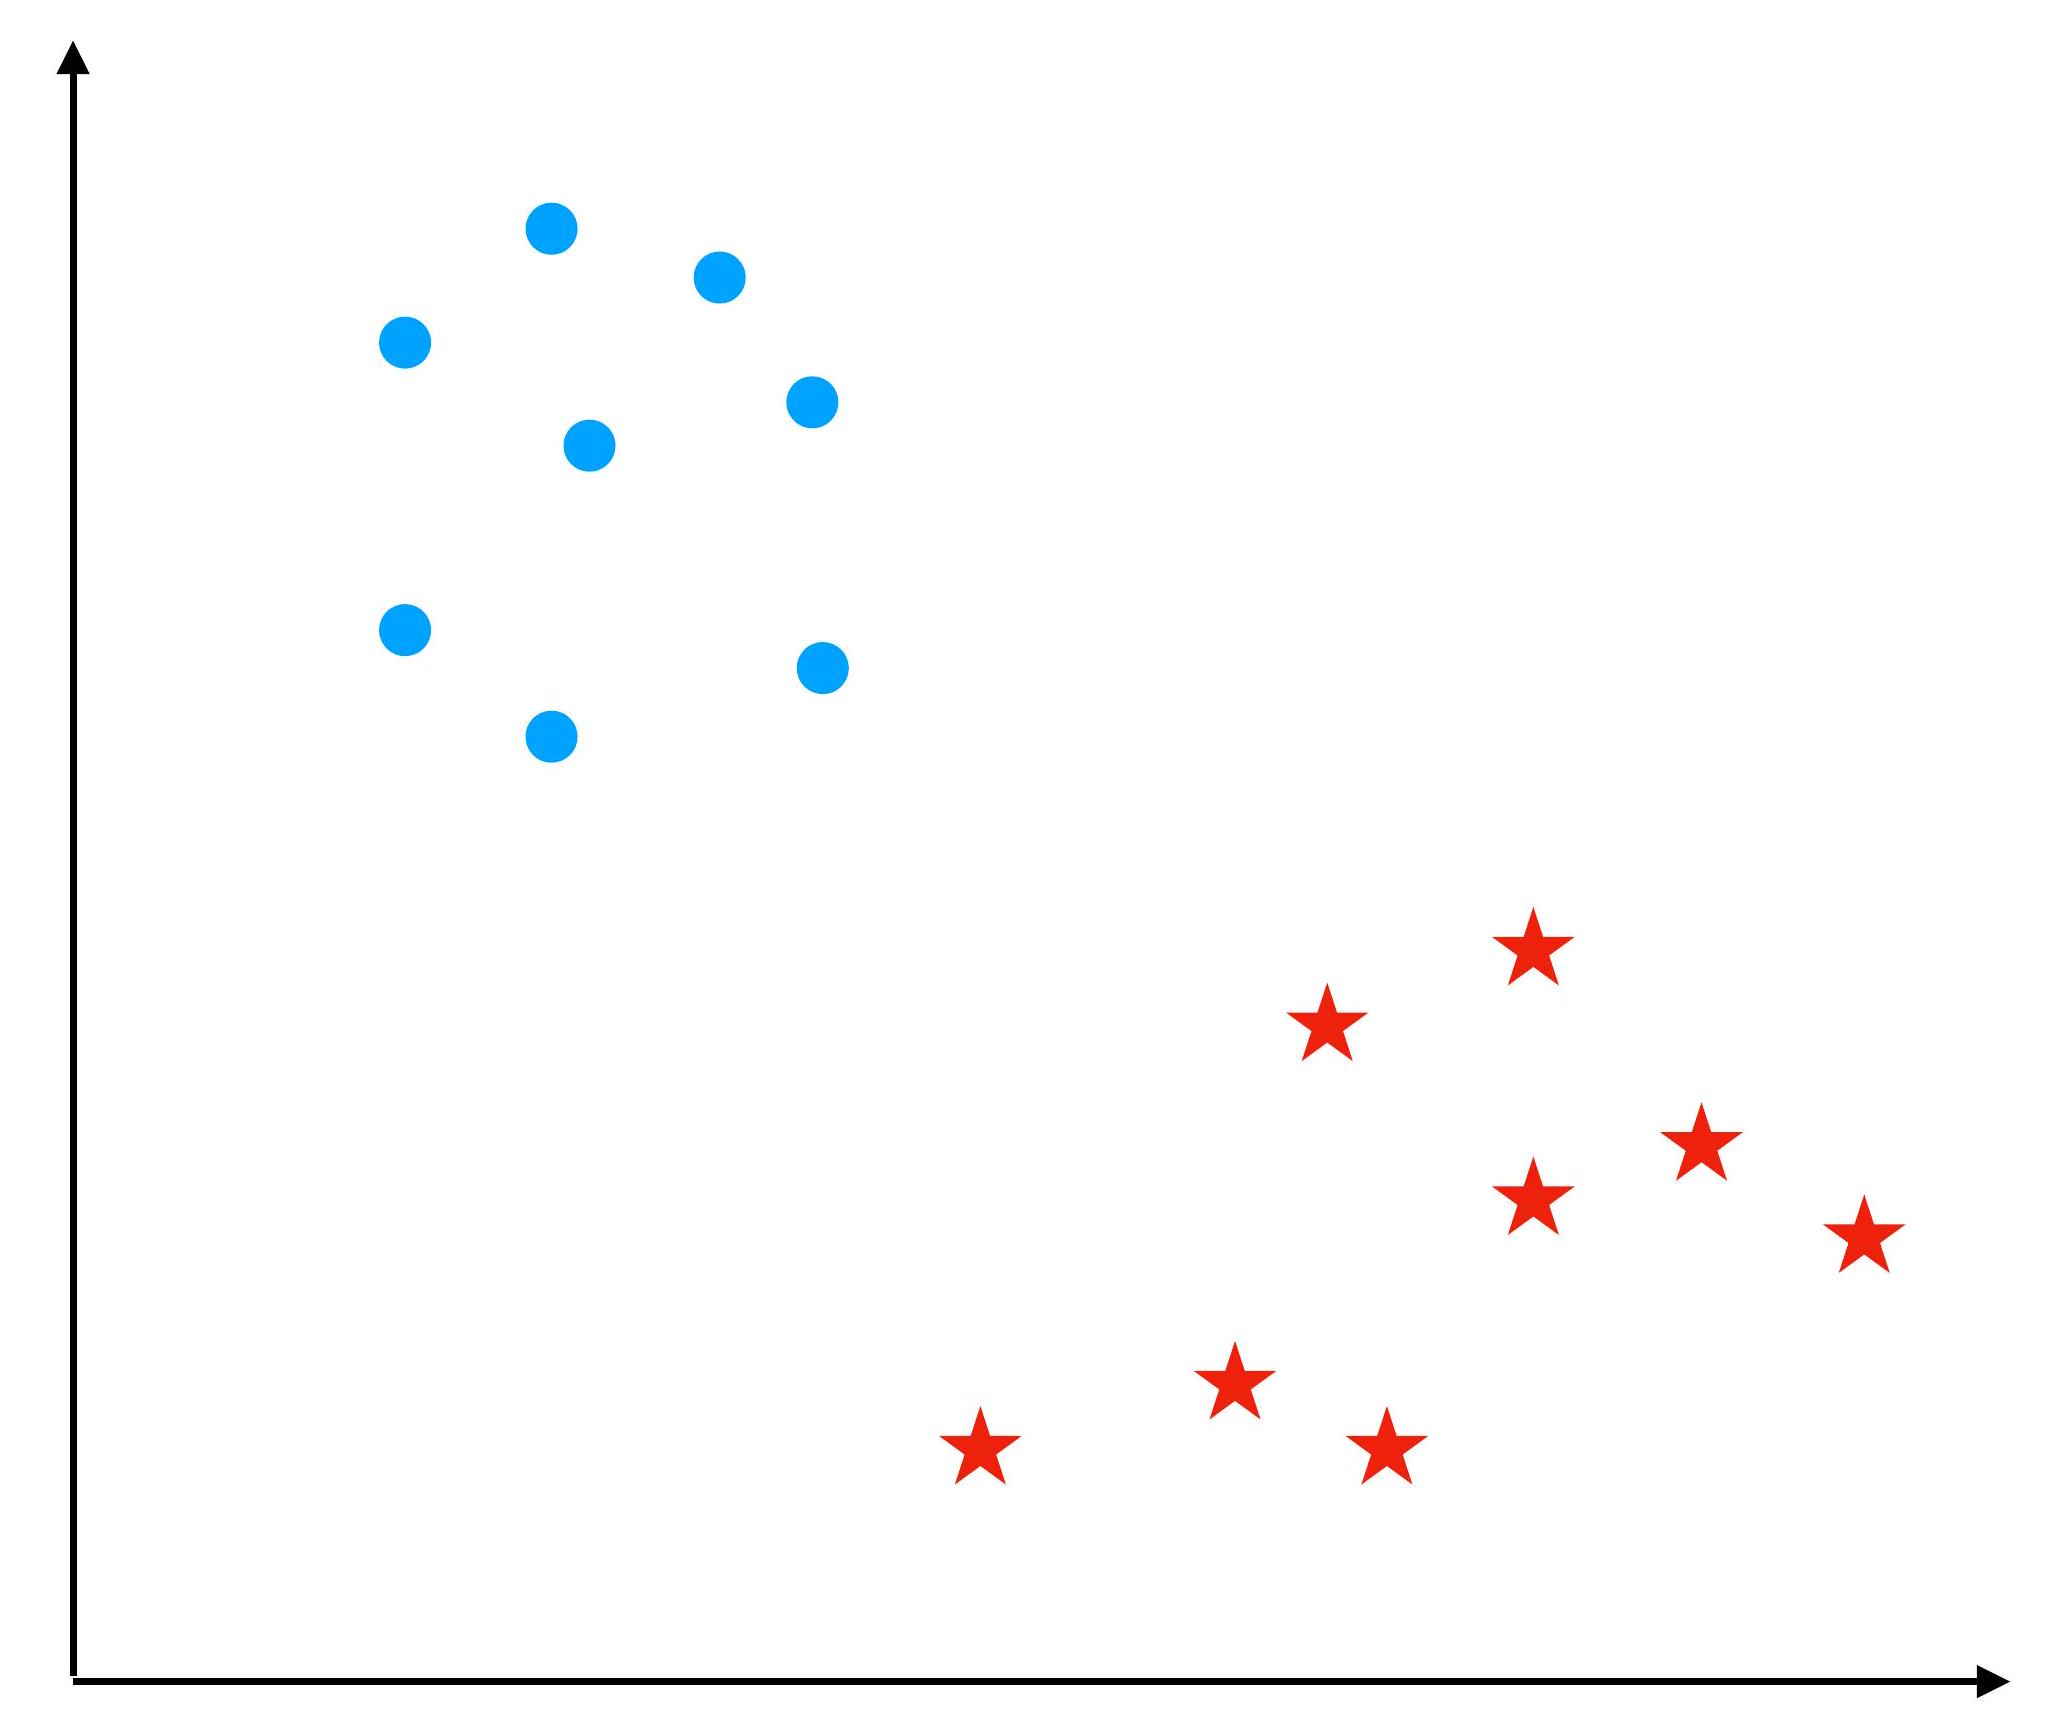
\includegraphics[max width=\textwidth]{2023_12_30_cf784c471dfd1dd5afbag-21}
\end{center}

Which separating hyperplane would you pick?

\section*{Margin}
Key concept: The margin is the distance from the hyperplane to the closest point

\begin{center}
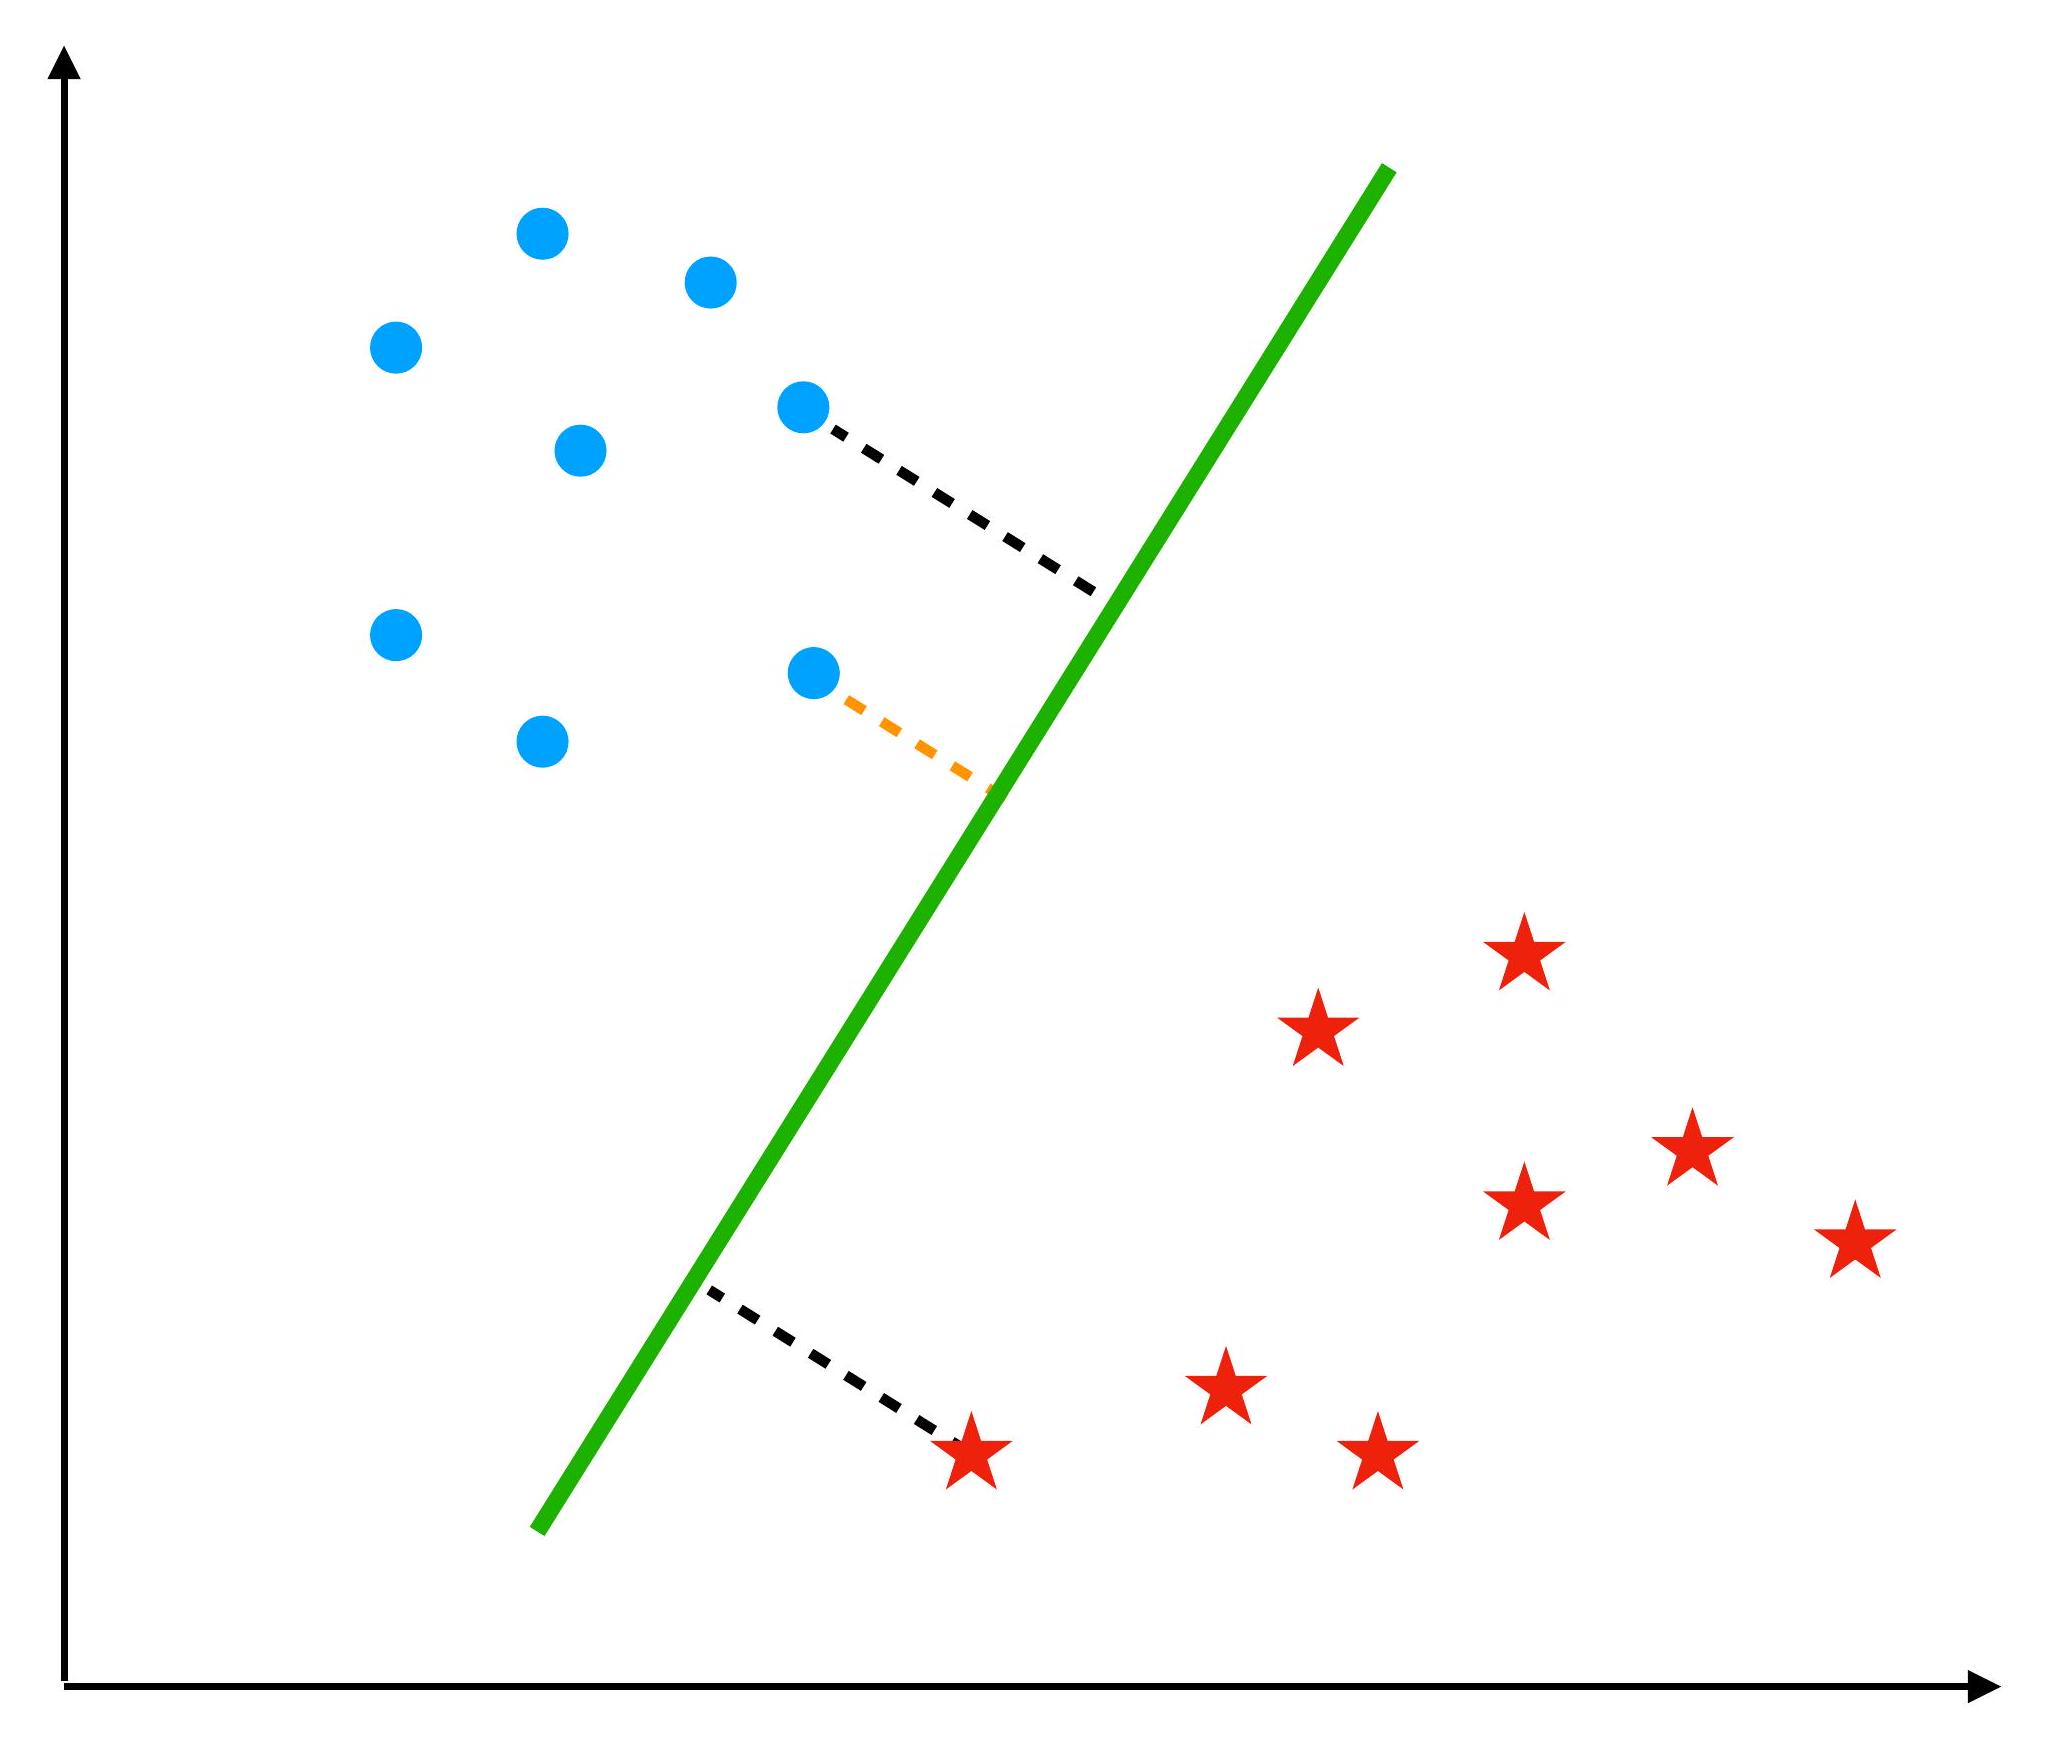
\includegraphics[max width=\textwidth]{2023_12_30_cf784c471dfd1dd5afbag-22}
\end{center}

$\Rightarrow$ Take the one with the largest margin!

\section*{Max-margin separating hyperplane}
Choose the hyperplane which maximizes the margin

\begin{center}
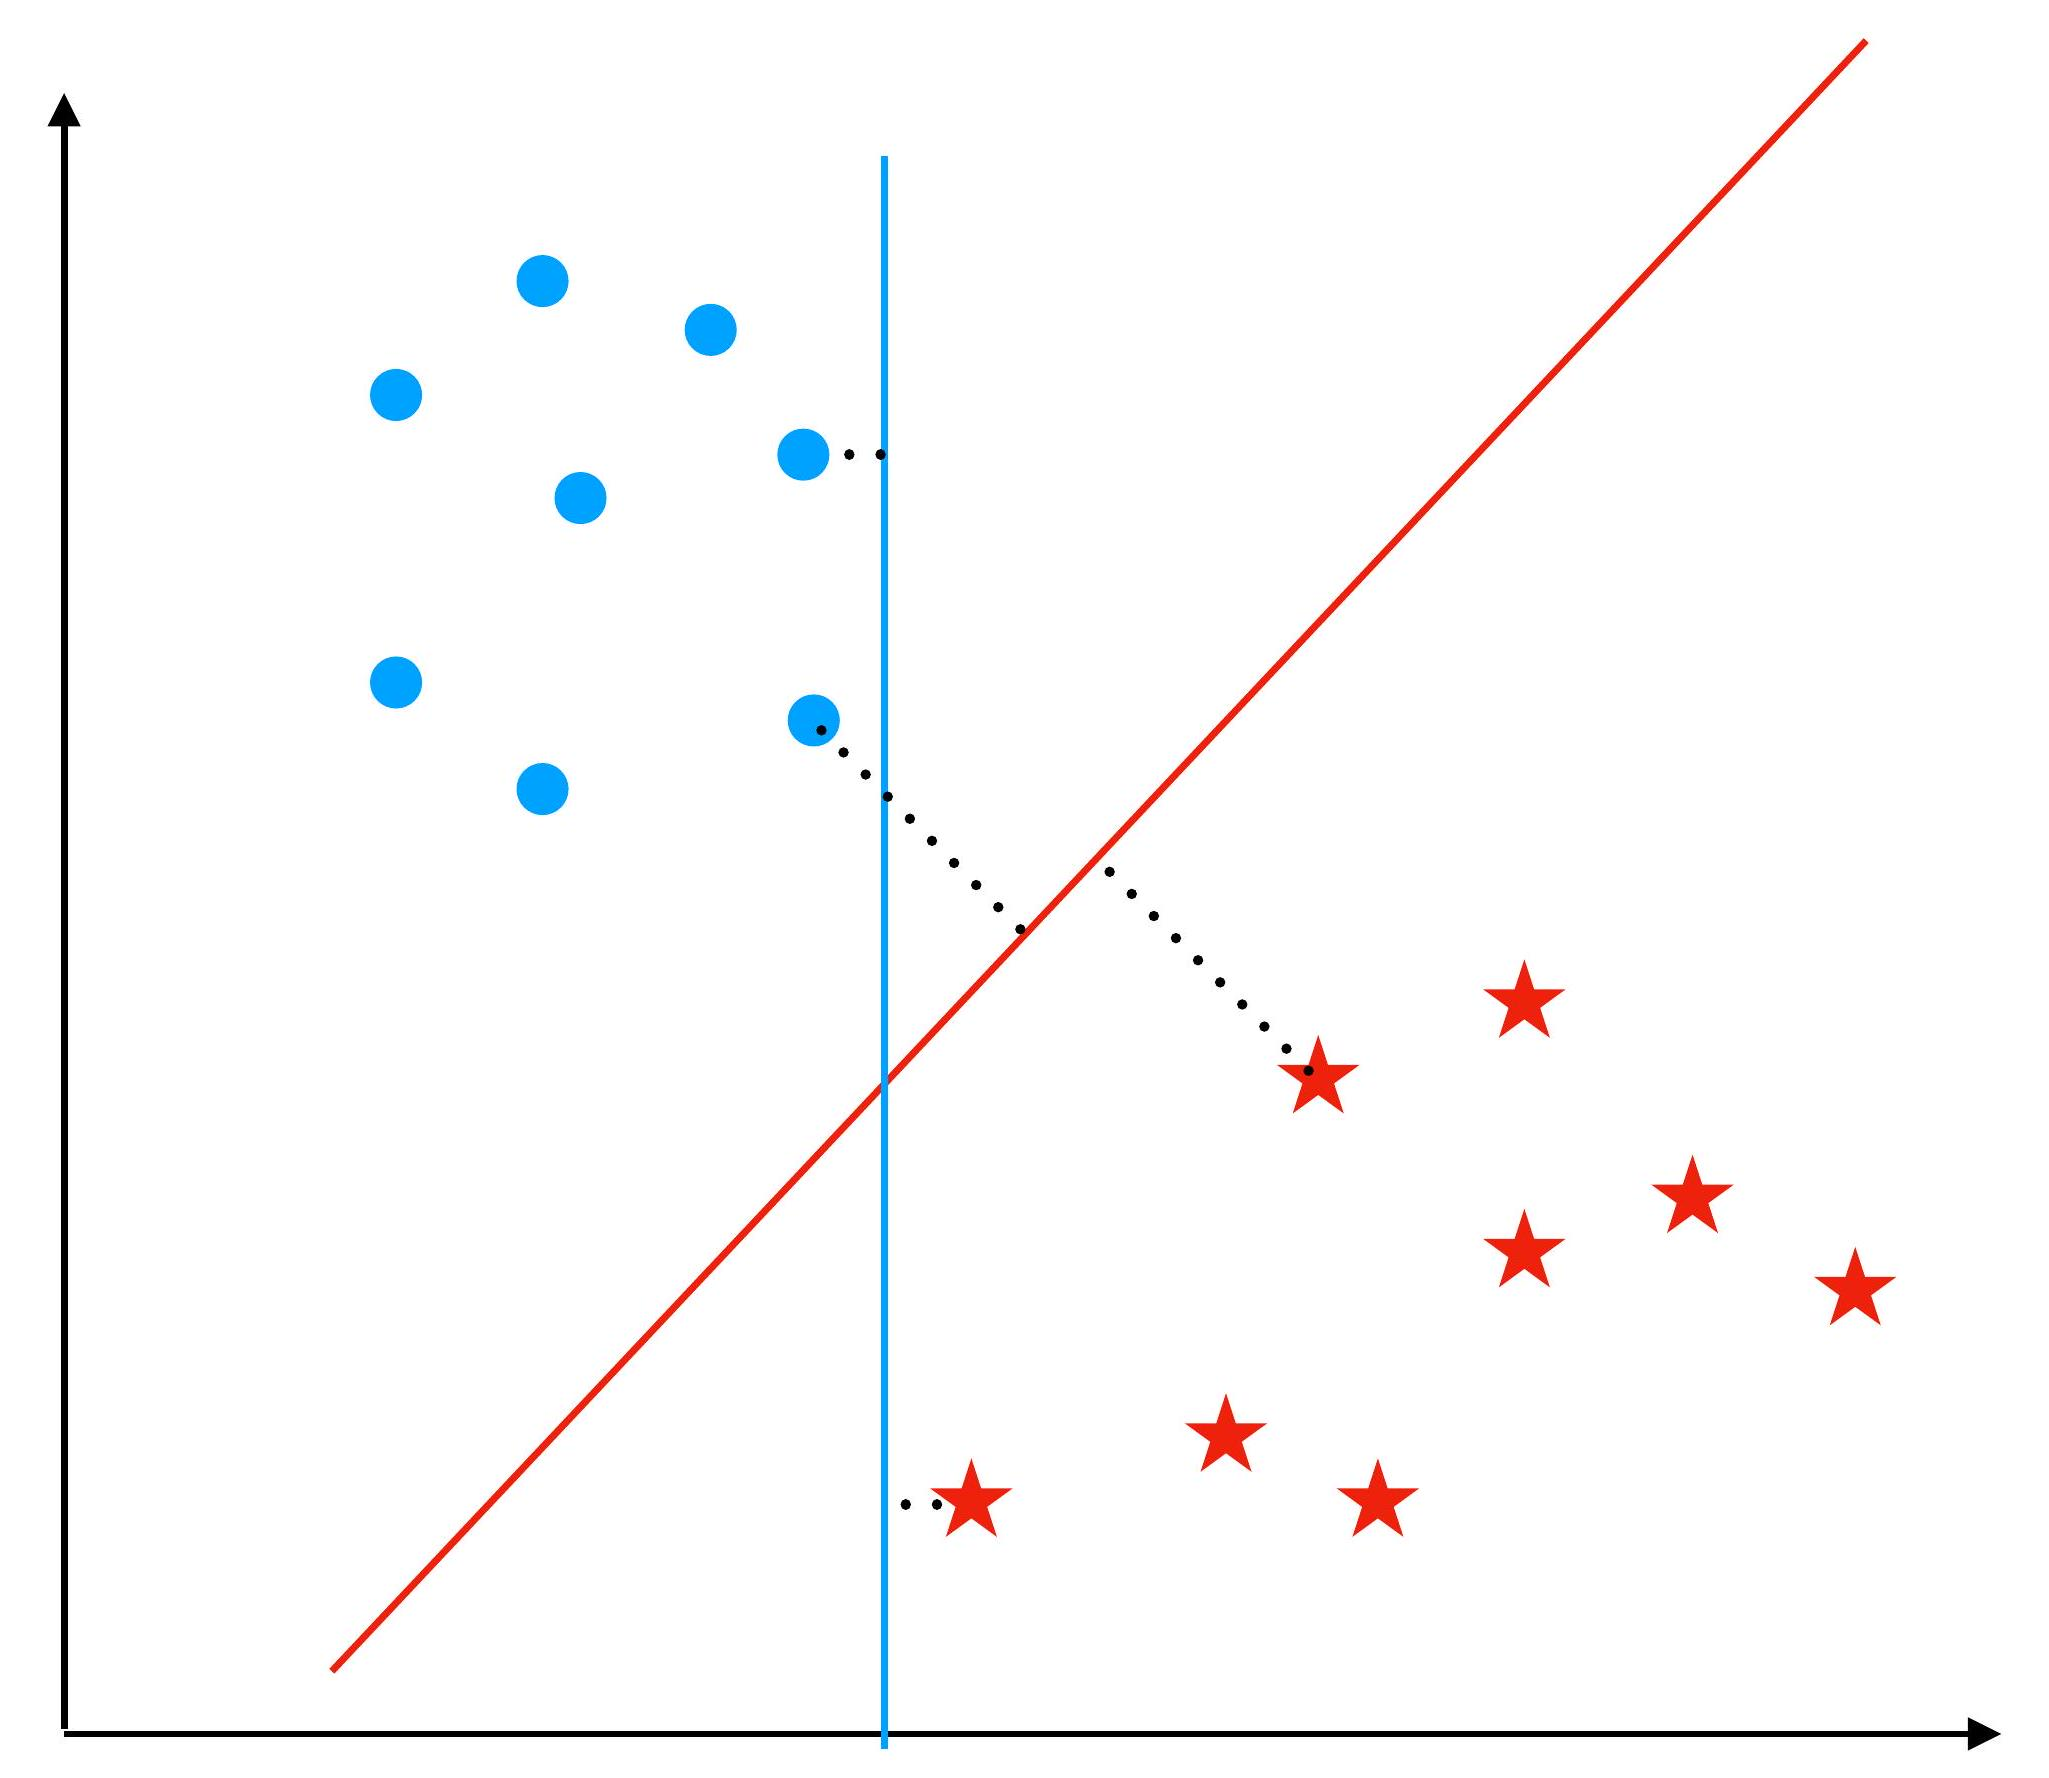
\includegraphics[max width=\textwidth]{2023_12_30_cf784c471dfd1dd5afbag-23}
\end{center}

Why: If we slightly change the training set, the number of misclassifications will stay low

$\Rightarrow$ It will lead us to support vector machine (SVM) and logistic regression

\section*{Nonlinear classifier}
\begin{itemize}
  \item Linear decision boundaries will not always work
\end{itemize}

\begin{center}
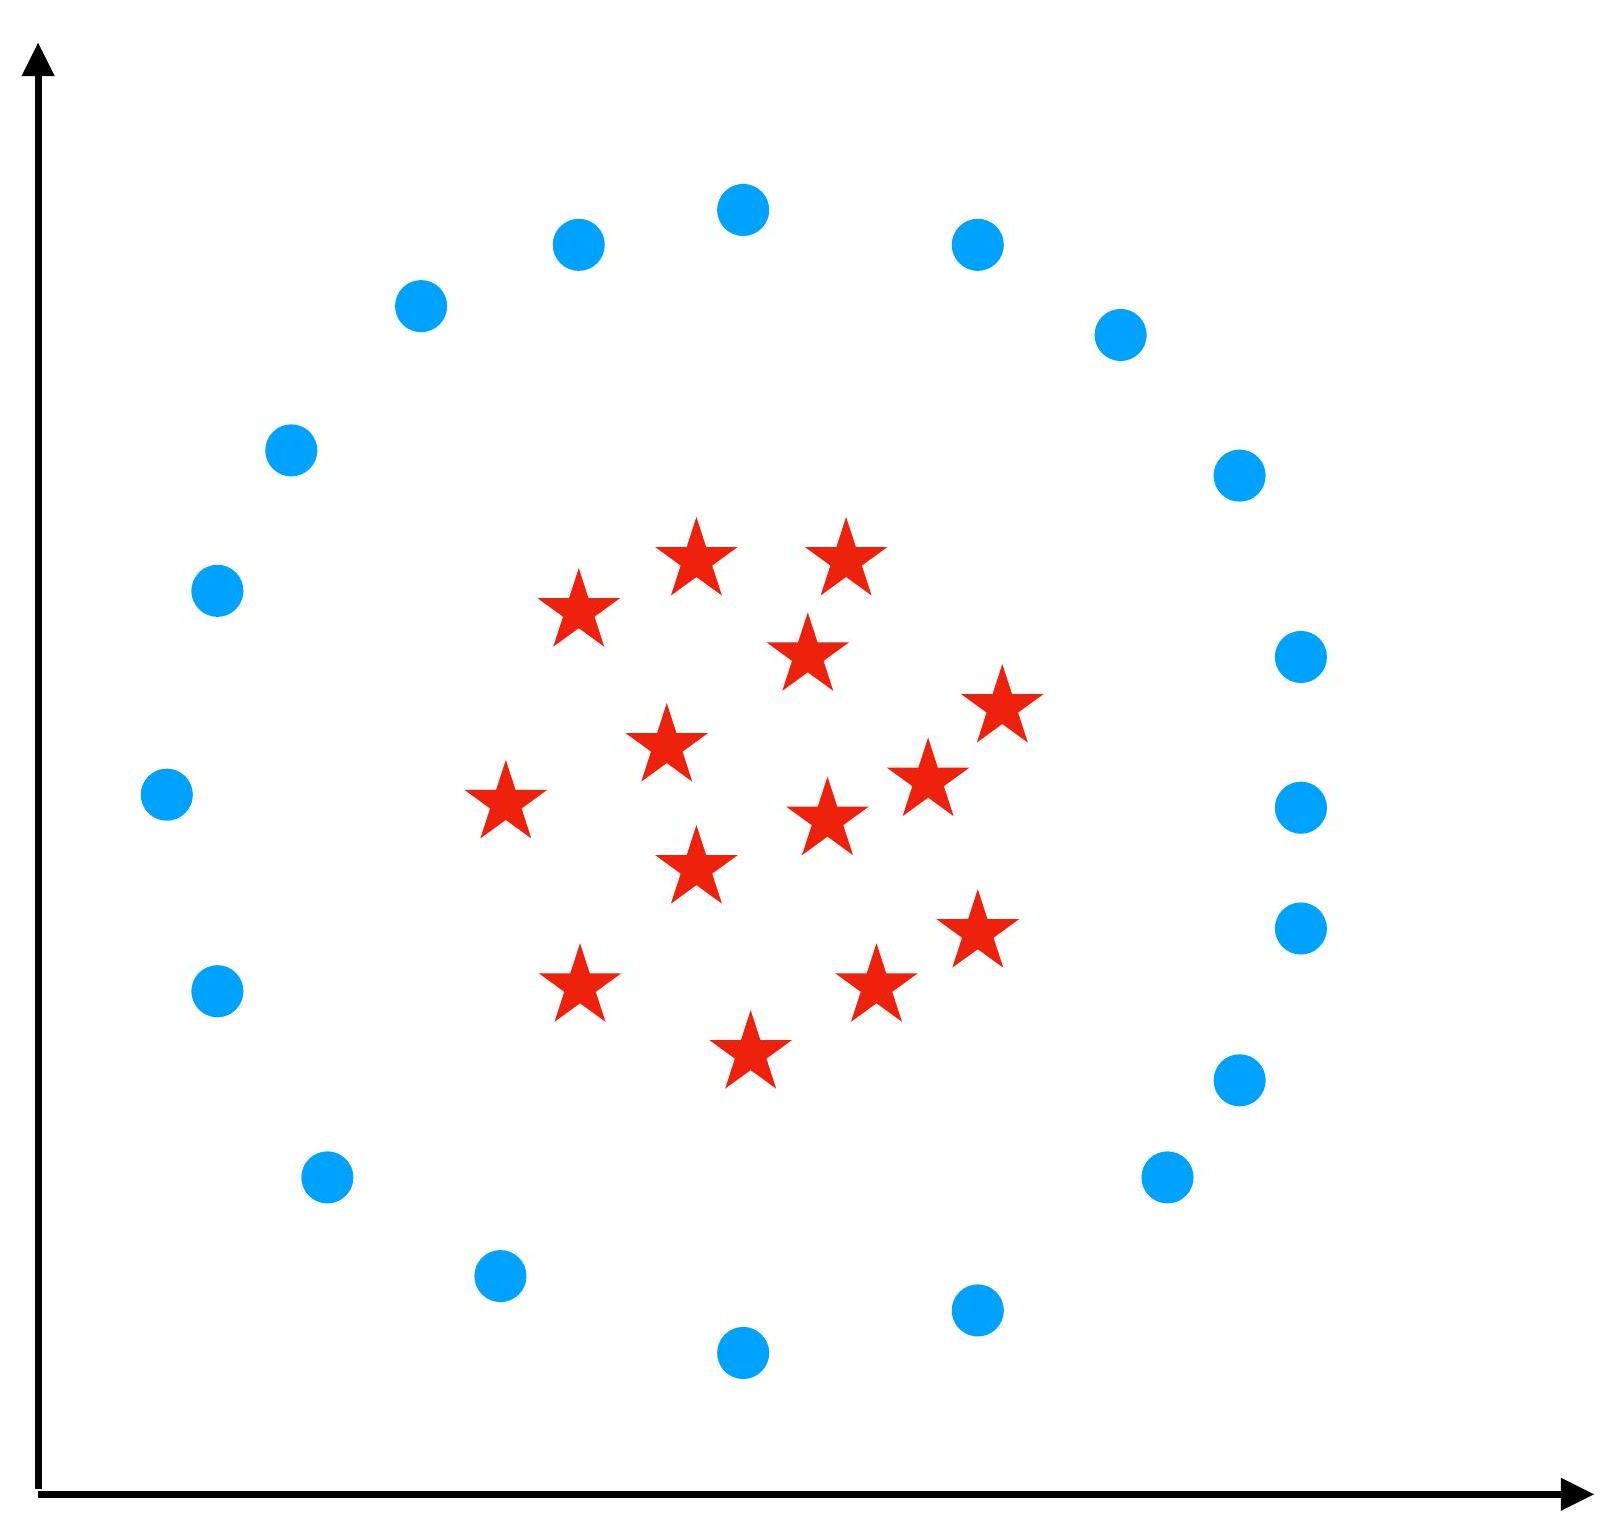
\includegraphics[max width=\textwidth]{2023_12_30_cf784c471dfd1dd5afbag-24}
\end{center}

\section*{Nonlinear classifier}
\begin{itemize}
  \item Linear decision boundaries will not always work

  \item Feature augmentation $\left(x, x^{2}, x^{3}, x^{4}\right)$

\end{itemize}

\begin{center}
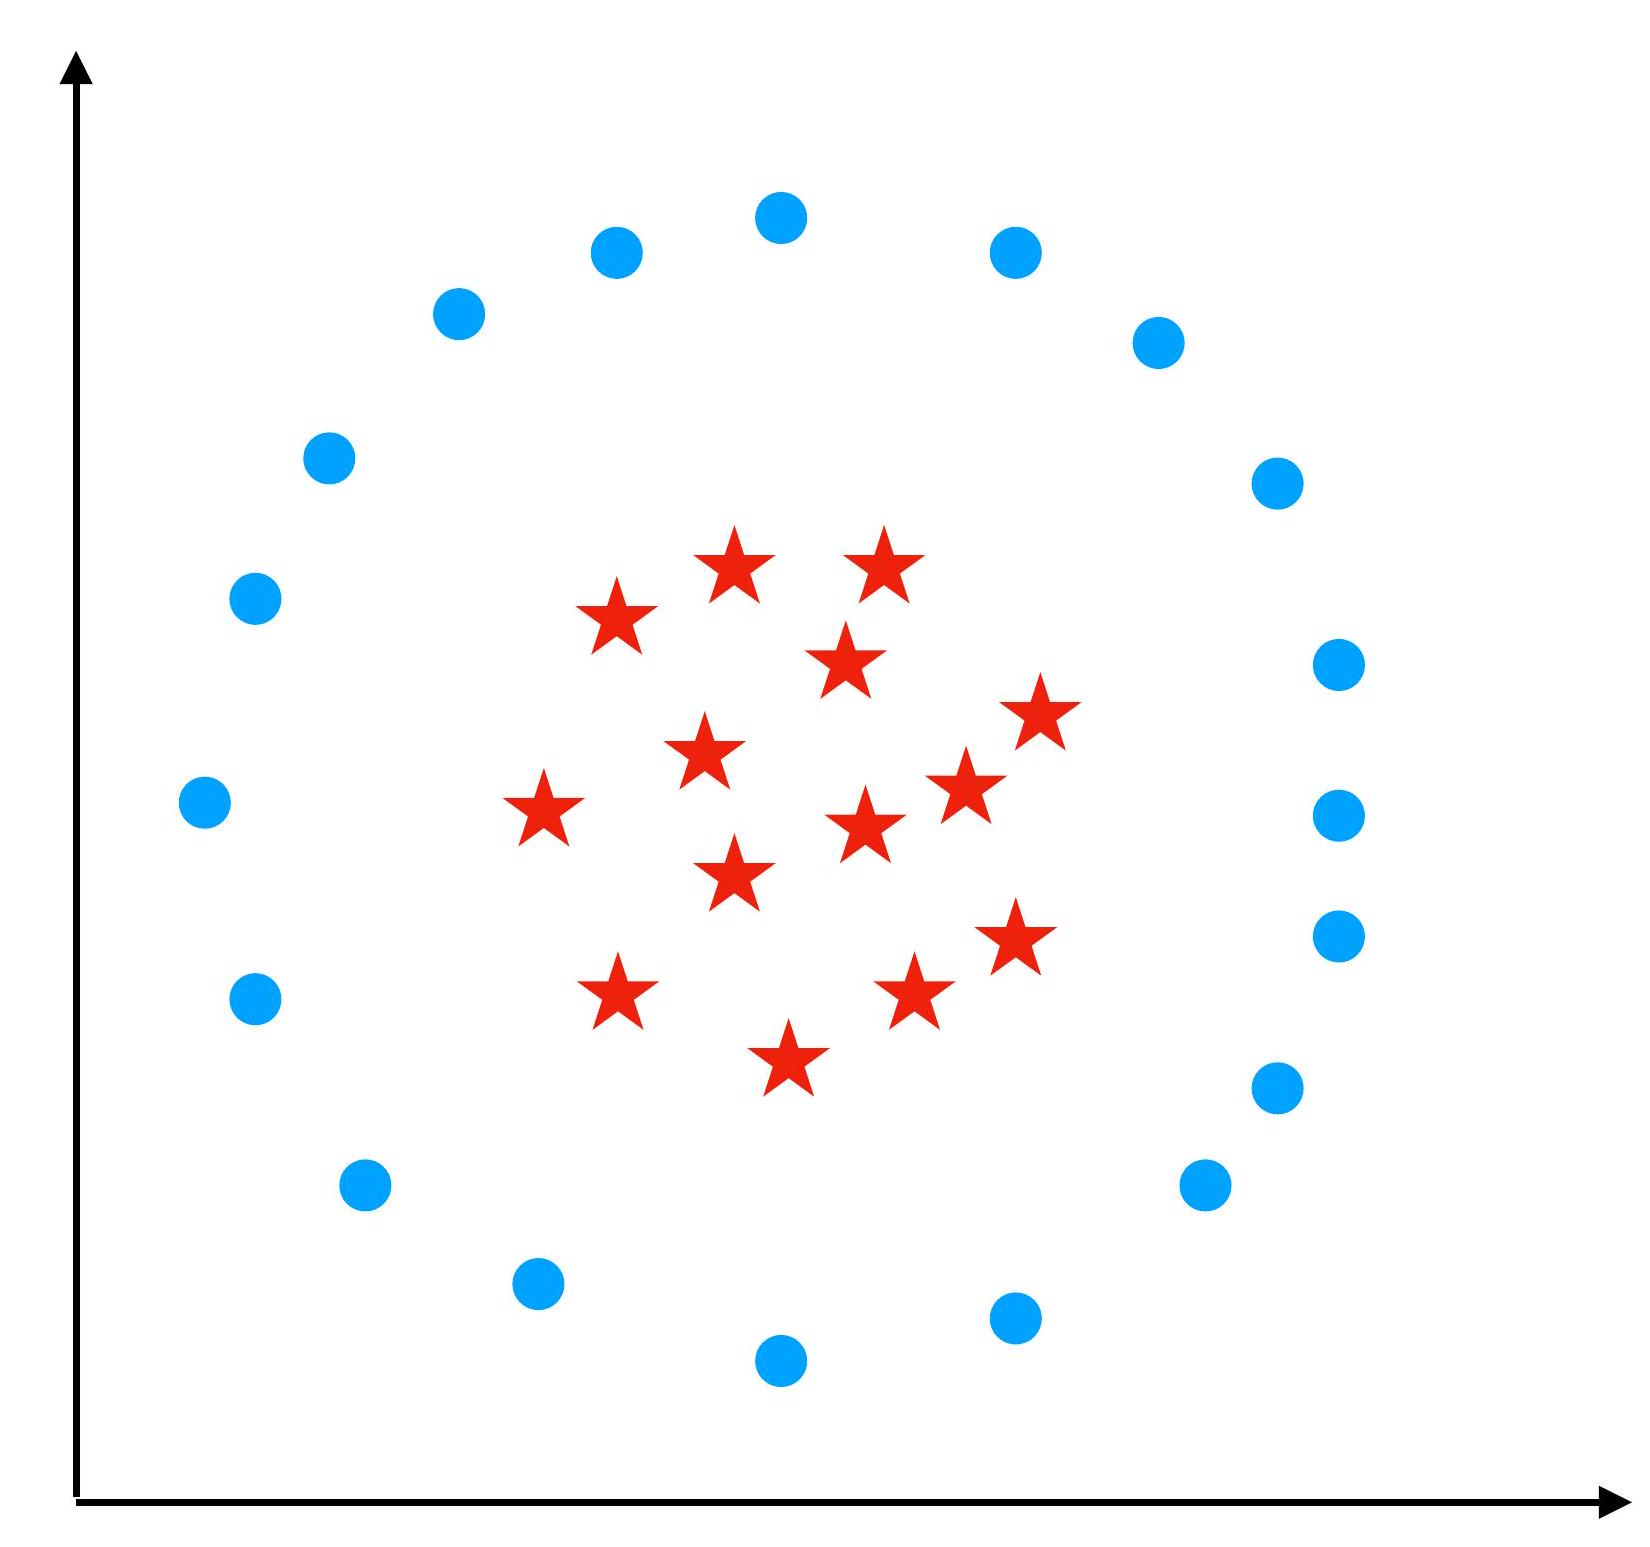
\includegraphics[max width=\textwidth]{2023_12_30_cf784c471dfd1dd5afbag-25}
\end{center}

\section*{Nonlinear classifier}
\begin{itemize}
  \item Linear decision boundaries will not always work

  \item Feature augmentation $\left(x, x^{2}, x^{3}, x^{4}\right)$

  \item Kernel Method

\end{itemize}

\begin{center}
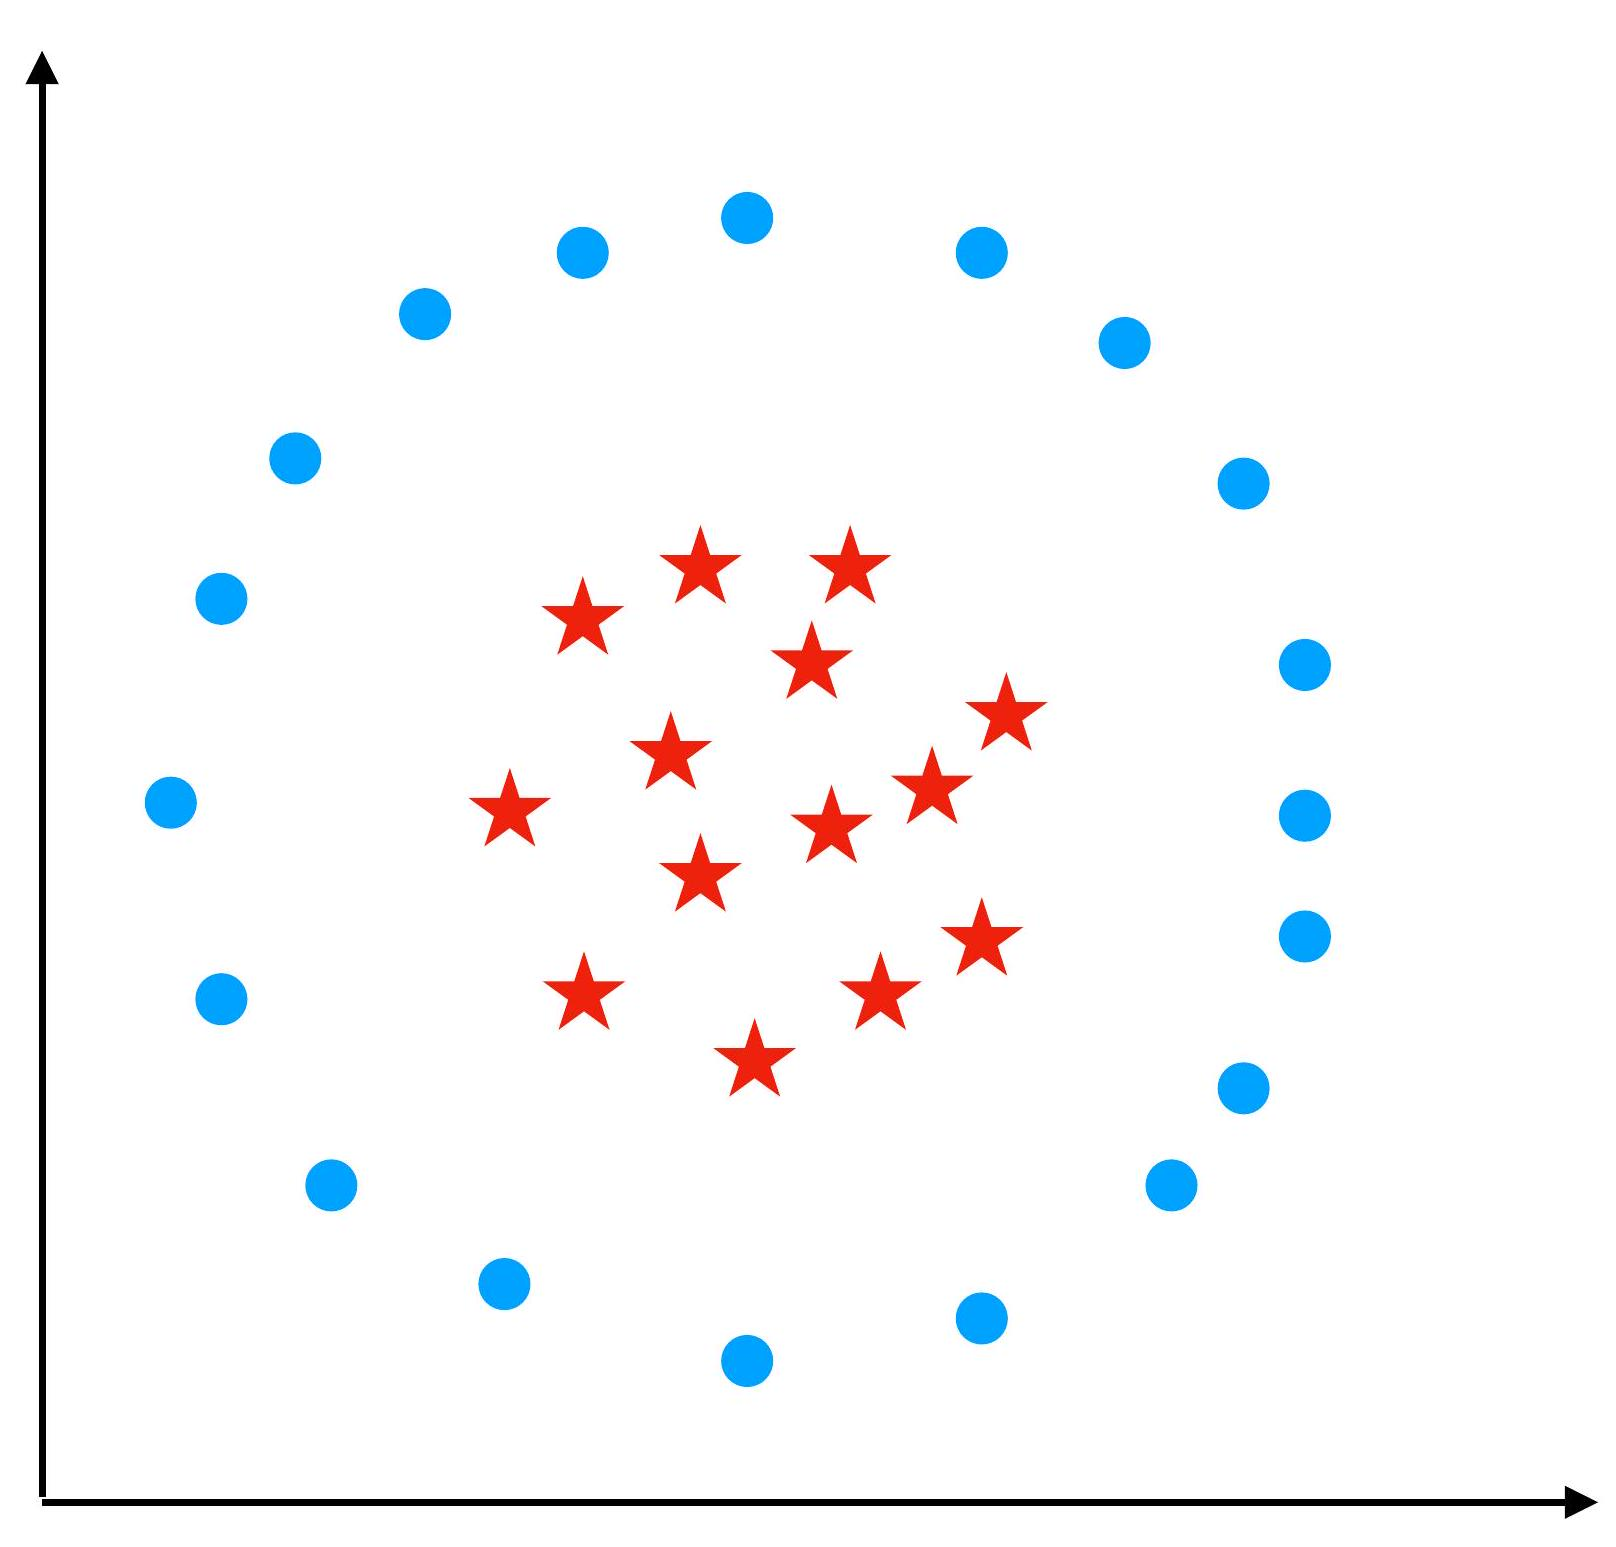
\includegraphics[max width=\textwidth]{2023_12_30_cf784c471dfd1dd5afbag-26}
\end{center}

\section*{Formalizing Binary Classification}
Setting: $(X, Y) \sim \mathscr{D}$ with ranges $\mathscr{X}, \mathscr{Y}=\{-1,1\}$

Loss function: (0-1 Loss) $\ell\left(y, y^{\prime}\right)=1_{y \neq y^{\prime}}= \begin{cases}1 & \text { if } y \neq y^{\prime} \\ 0 & \text { if } y=y^{\prime}\end{cases}$

True risk for the classification:

$$
\begin{aligned}
& \quad L_{\mathscr{D}}(f)=\mathbb{E}_{\mathscr{D}}\left[1_{Y \neq f(X)}\right]=\mathbb{P}_{\mathscr{D}}[Y \neq f(X)] \\
& \text { classification error }
\end{aligned}
$$

Goal: minimize $L_{\mathscr{D}}(f)$

\section*{Bayes classifier}
What is the optimal performance, regardless of the finiteness of the training data?

Def: The classifier $f_{*}=\arg \min L_{\mathscr{D}}(f)$ is called the Bayes classifier $f$

Claim:

$$
f_{*}(x)=\arg \max _{y \in\{-1,1\}} \mathbb{P}(Y=y \mid X=x)
$$

Note: Bayes classifier is an unattainable gold standard, as we never know the underlying data distribution $\mathscr{D}$ in practice

\section*{Proof of the Bayes classifier}
Claim 1: $\forall x \in \mathscr{X}, f_{*}(x) \in \arg \min _{y \in \mathscr{Y}} \mathbb{P}(Y \neq y \mid X=x) \Longrightarrow f_{*} \in \arg \min _{f: \mathscr{X} \rightarrow \mathscr{Y}} L_{\mathscr{D}}(f)$

$$
\begin{aligned}
L_{\mathscr{D}}(f)=\mathbb{E}_{X, Y}\left[1_{Y \neq f(X)}\right] & =\mathbb{E}_{X}\left[\mathbb{E}_{Y \mid X}\left[1_{Y \neq f(X)} \mid X\right]\right] \\
& =\mathbb{E}_{X}[\mathbb{P}(Y \neq f(X) \mid X)] \\
& \geq \mathbb{E}_{X}\left[\min _{y \in \mathscr{Y}} \mathbb{P}(Y \neq y \mid X)\right] \\
& =\mathbb{E}_{X}\left[\mathbb{P}\left(Y \neq f_{*}(X) \mid X\right)\right]=\mathbb{E}_{X, Y}\left[1_{Y \neq f_{*}(X)}\right]=L_{\mathscr{D}}\left(f_{*}\right)
\end{aligned}
$$

Claim 2: $f_{*}(x)=\arg \min _{y \in \mathscr{Y}} \mathbb{P}(Y \neq y \mid X=x)$

$$
f_{*}(x)=\arg \max _{y \in \mathscr{Y}} \mathbb{P}(Y=y \mid X=x)=\arg \min _{y \in \mathscr{Y}} \mathbb{P}(Y \neq y \mid X=x)
$$

\section*{Two classes of classification algorithms}
\begin{itemize}
  \item Non-parametric: approximate the conditional distribution $\mathbb{P}(Y=y \mid X=x)$ via local averaging
\end{itemize}

$\Rightarrow$ Follow nearest neighbors' decisions (KNN)

\begin{itemize}
  \item Parametric: approximate true distribution $\mathscr{D}$ via training data
\end{itemize}

$\Rightarrow$ Minimize the empirical risk on training data (ERM)

\section*{Classification by empirical risk minimization}
How: minimize the empirical risk instead of the true risk:

$$
\min _{f: X \rightarrow Y} L_{\operatorname{train}}(f):=\frac{1}{N} \sum_{n=1}^{N} 1_{f\left(x_{n}\right) \neq y_{n}}=\frac{1}{N} \sum_{n=1}^{N} 1_{y_{n} f\left(x_{n}\right) \leq 0}
$$

Problem: $L_{\text {train }}$ is not convex:

\begin{enumerate}
  \item The set of classifiers is not convex because $\mathcal{Y}$ is discrete

  \item The indicator function 1 is not convex because it is not continuous

\end{enumerate}

\section*{Convex relaxation of the classification risk}
\begin{enumerate}
  \item Instead of learning $f: \mathscr{X} \rightarrow \mathscr{Y}$, learn $g: \mathscr{X} \rightarrow \mathbb{R}$ in a convex subset of continuous functions $\mathscr{G}$, and predict with $f(x)=\operatorname{sign}(g(x))$. The problem becomes
\end{enumerate}

$$
\min _{g \in \mathscr{G}} \frac{1}{N} \sum_{n=1}^{N} 1_{y_{n} g\left(x_{n}\right) \leq 0}
$$

\begin{enumerate}
  \setcounter{enumi}{1}
  \item Replace the indicator function by a convex $\phi: \mathbb{R} \rightarrow \mathbb{R}$ and minimize
\end{enumerate}

$$
\min _{g \in \mathscr{G}} \frac{1}{N} \sum_{n=1}^{N} \phi\left(y_{n} g\left(x_{n}\right)\right)
$$

$\phi$ is a function of the functional margin $y_{n} g\left(x_{n}\right)$

$\Rightarrow$ This is a convex problem!

\begin{center}
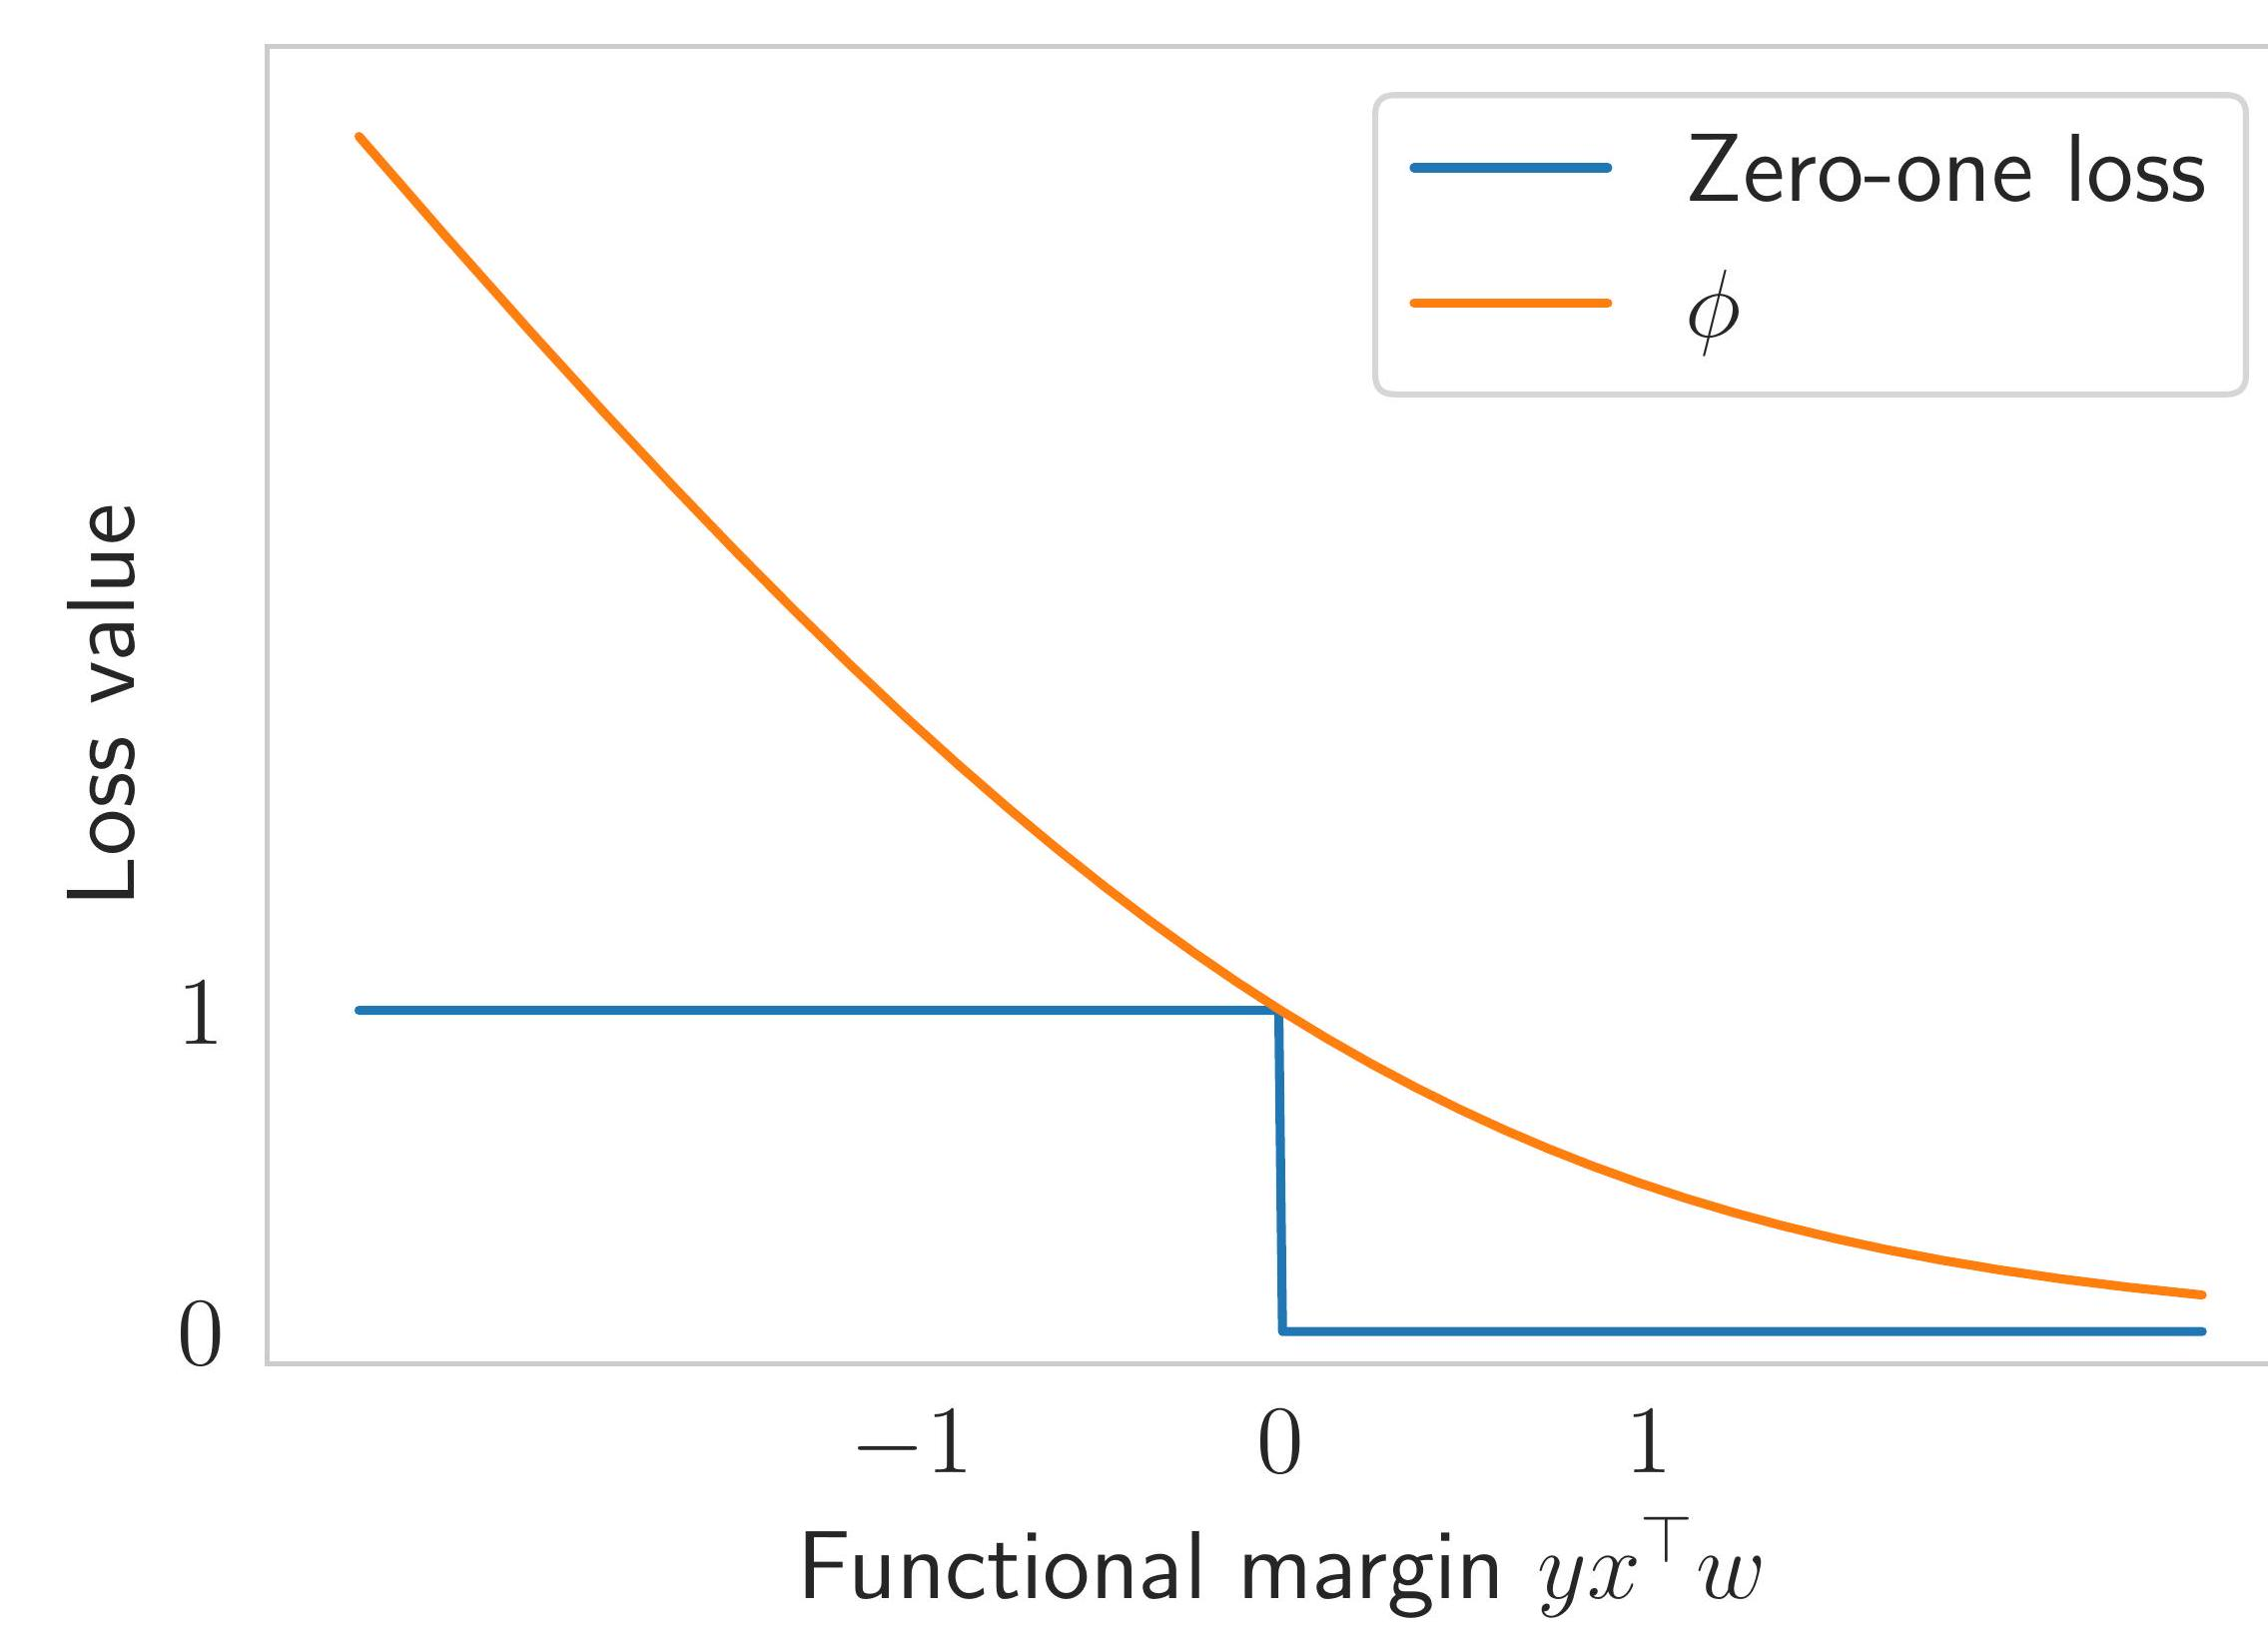
\includegraphics[max width=\textwidth]{2023_12_30_cf784c471dfd1dd5afbag-32}
\end{center}

Remark: possible to bound the zero-one risk $L(f)$ by the $\phi$ risk *

\section*{Losses for Classification}
\begin{center}
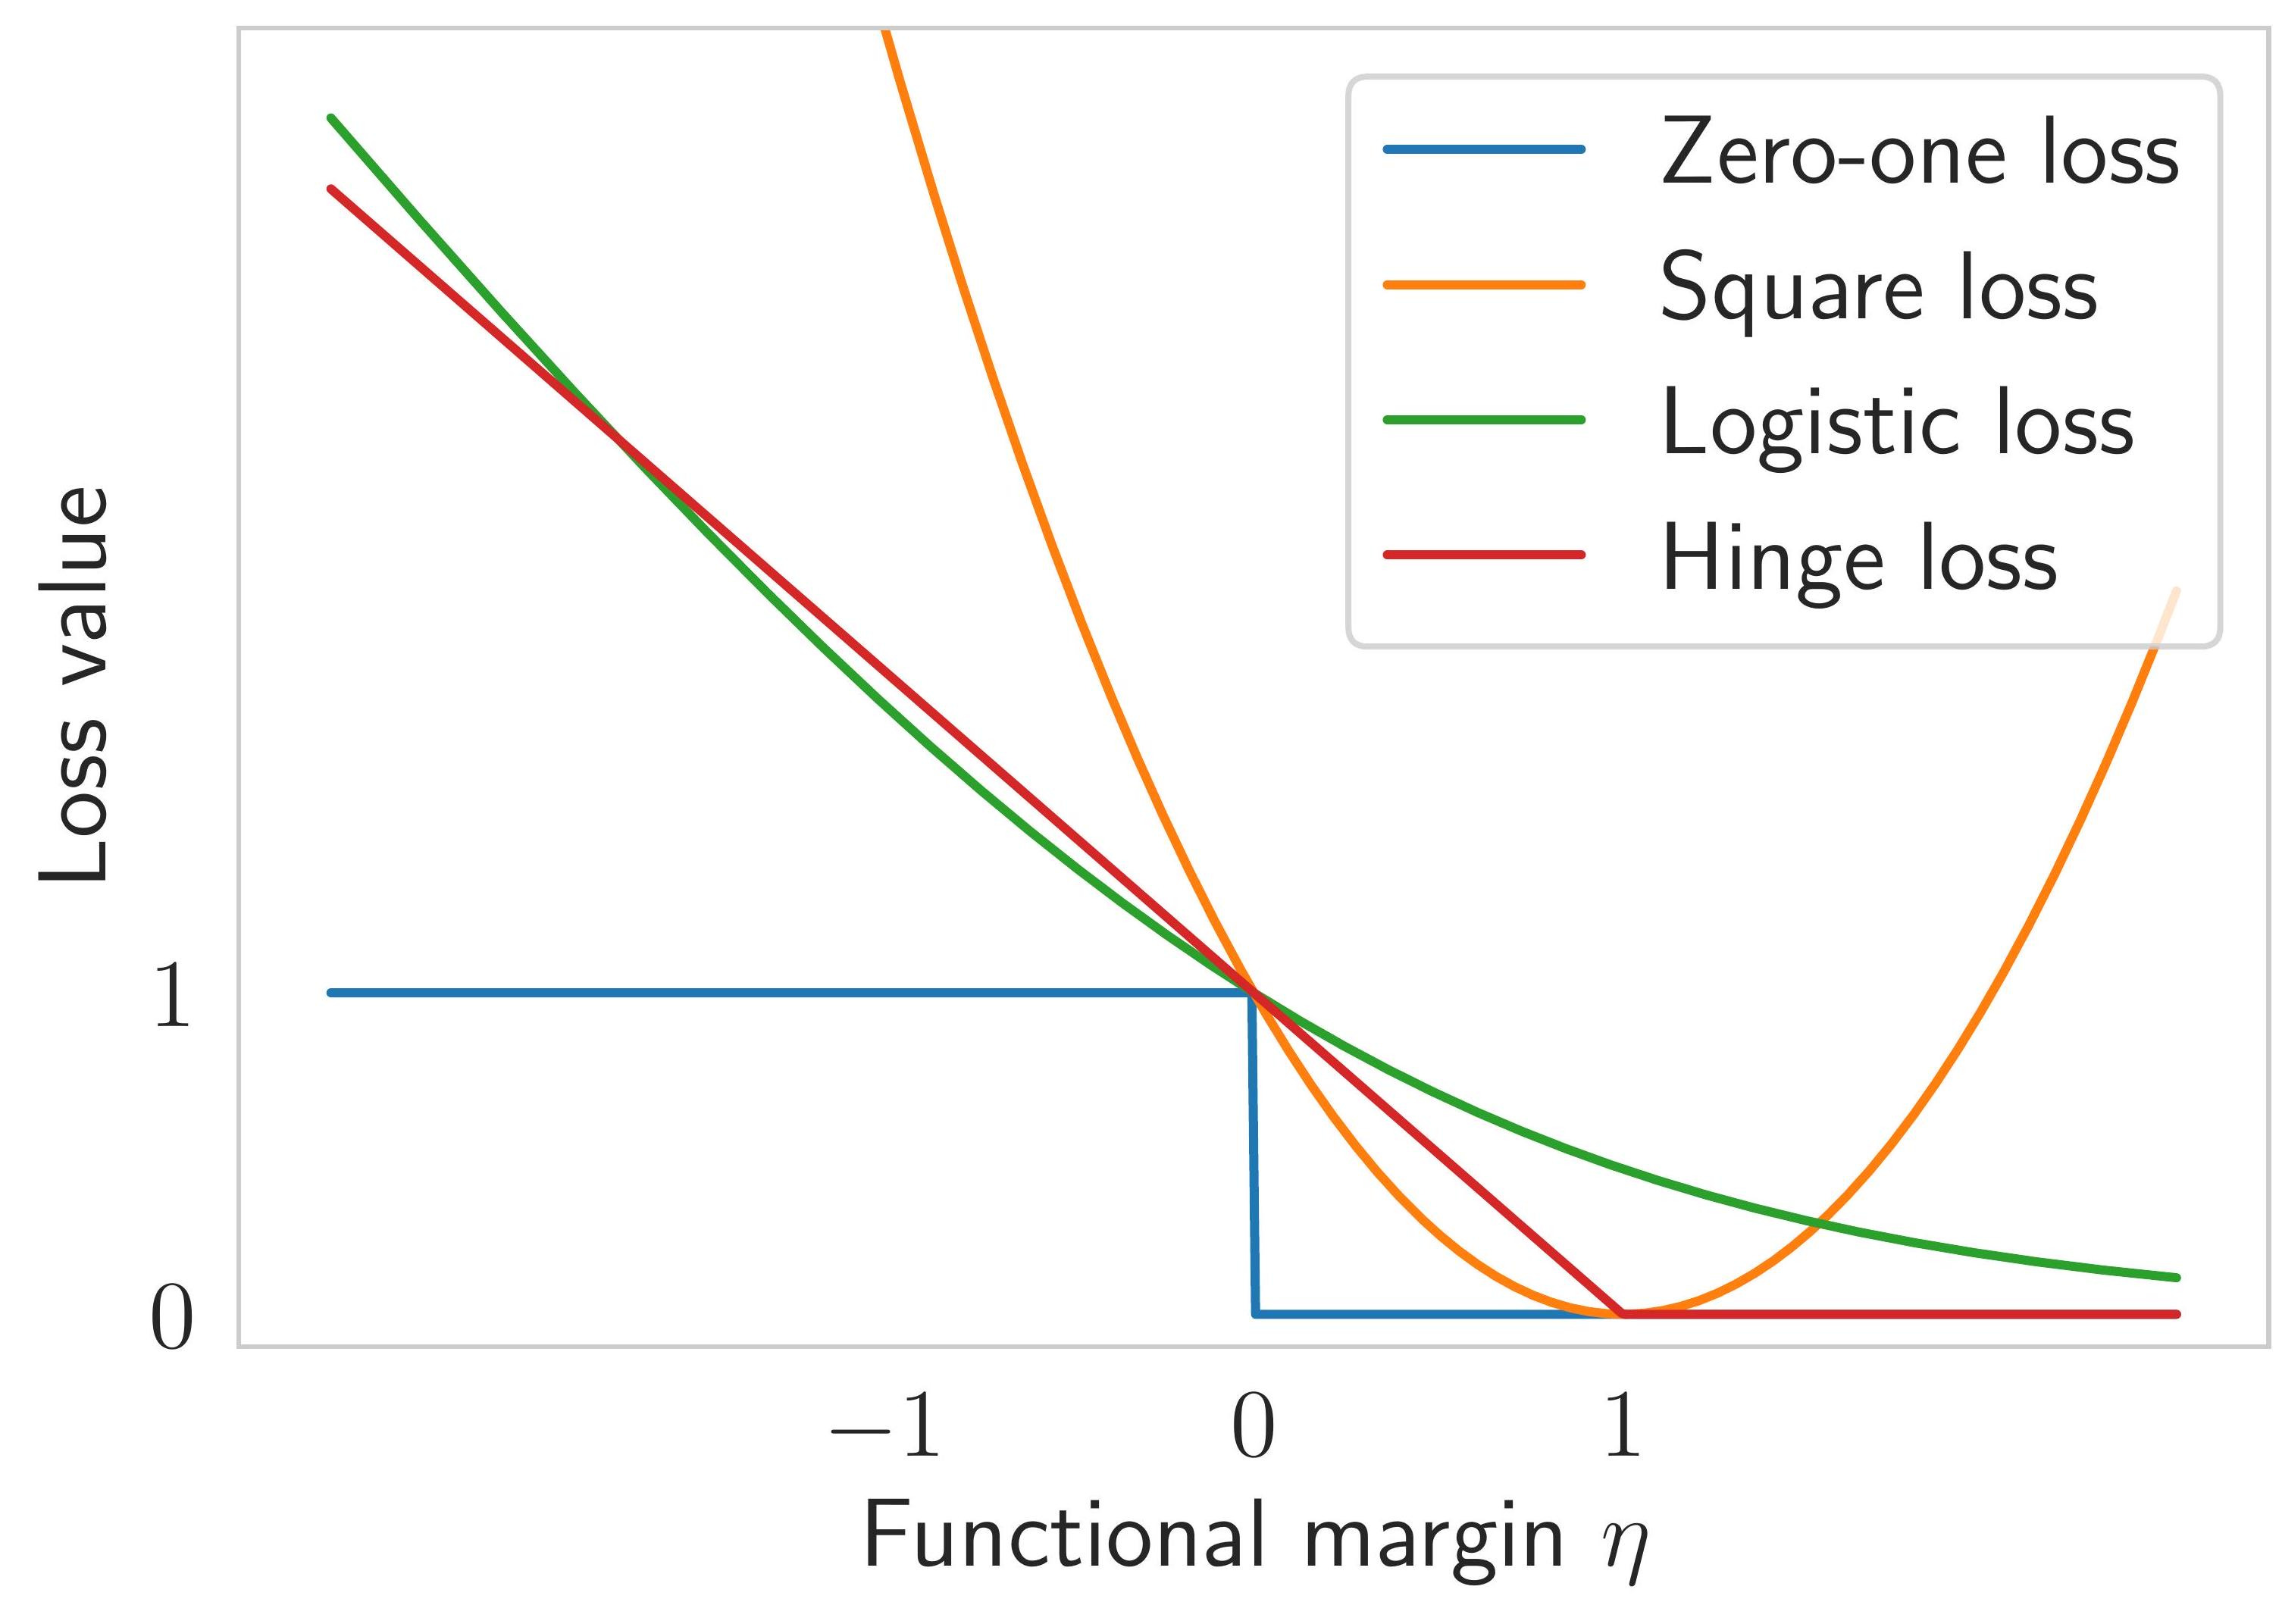
\includegraphics[max width=\textwidth]{2023_12_30_cf784c471dfd1dd5afbag-33}
\end{center}

Logistic loss $\rightarrow$ logistic regression

Hinge loss $\rightarrow$ max margin classification

\section*{Do we still have time?}
\section*{Bonus: a good regressor implies a good classifier}
Consider $\mathscr{Y}=\{0,1\}$, for all regression functions $\eta: \mathscr{X} \rightarrow \mathbb{R}$ we can define a classifier as

$$
\begin{aligned}
\mathscr{X} & \rightarrow\{0,1\} \\
f_{\eta}: x & \mapsto 1_{\eta(x) \geq 1 / 2}
\end{aligned}
$$

Claim:

$$
L_{\mathscr{D}}^{\text {classif }}\left(f_{\eta}\right)-L_{\mathscr{D}}^{\text {classif }}\left(f^{*}\right) \leq 2 \sqrt{L_{\mathscr{D}}^{\ell_{2}}(\eta)-L_{\mathscr{D}}^{\ell_{2}}\left(\eta^{*}\right)}
$$

Where $L_{\mathscr{D}}^{\text {classif }}\left(f_{\eta}\right)=\mathbb{E}_{\mathscr{D}}\left[1_{f(X) \neq Y}\right], L_{\mathscr{D}}^{\ell_{2}}(f)=\mathbb{E}_{\mathscr{D}}\left[(Y-f(X))^{2}\right]$ and $\eta_{*}=\arg \min _{\eta} L_{\mathscr{D}}^{\ell_{2}}(\eta)$

$\Rightarrow$ If $\eta$ is good for regression then $f_{\eta}$ is good for classification too (converse is not true)

\section*{Bonus: does the loss function matter? (Over-parameterization regime)}
Assume sufficient over-parameterization $(n \ll d)$, i.e. all training points are equally close to the separating hyperplane, with high probability

Optimization (training): the outcome of optimization with gradient descent, is the same for both logistic loss and square loss

With square loss: BERT

With cross-entropy: BERT

With square loss: LSTM+Attention

With cross-entropy: LSTM+Attention

With square loss: LSTM+CNN

With cross-entropy: LSTM+CNN

\begin{itemize}
  \item With cross-entropy: LSTM+CNN
\end{itemize}

\begin{center}
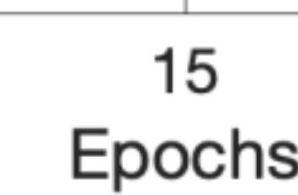
\includegraphics[max width=\textwidth]{2023_12_30_cf784c471dfd1dd5afbag-36(1)}
\end{center}

(a) NLP tasks

Training curves on ImageNet

\begin{center}
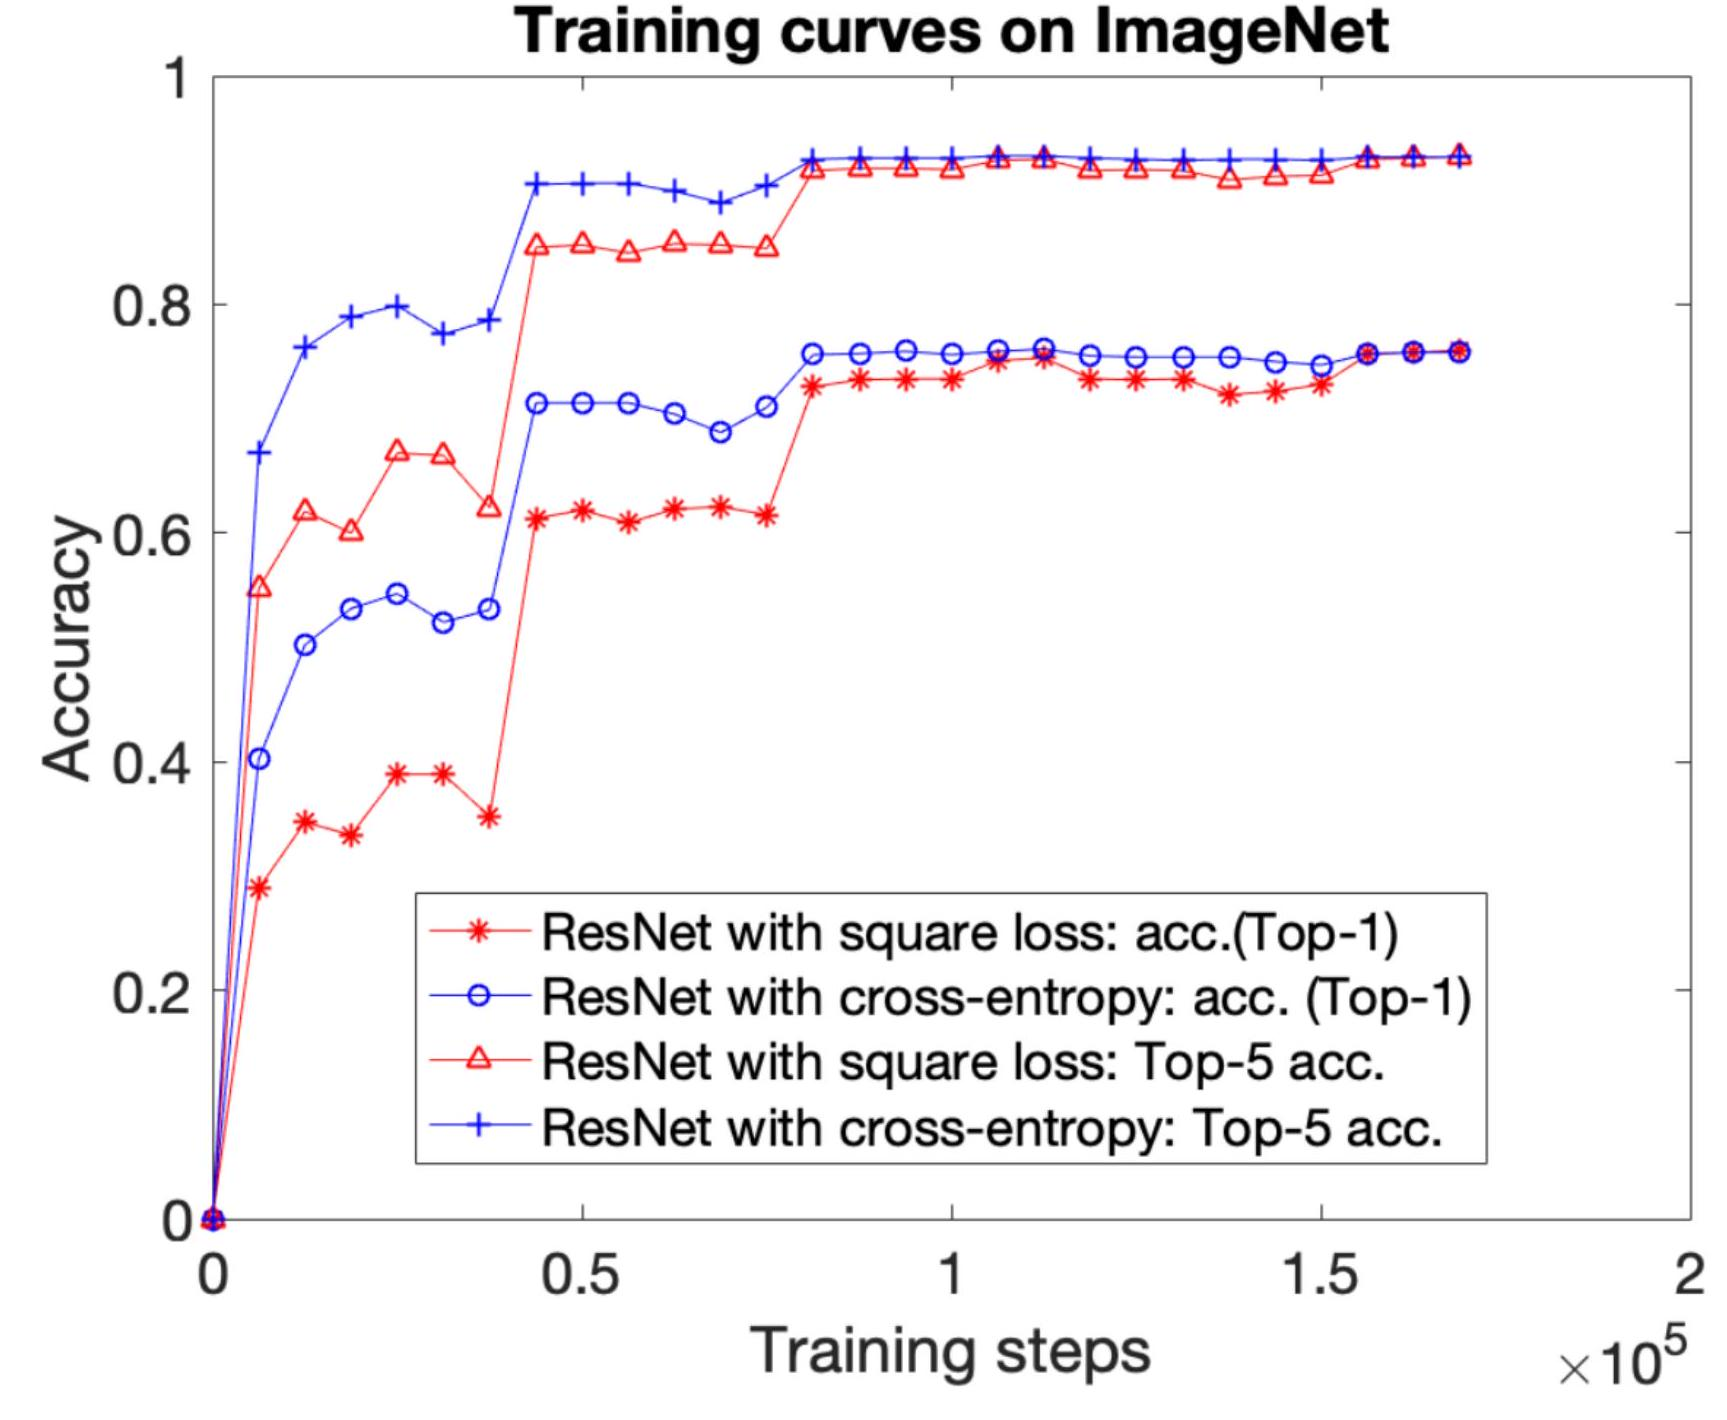
\includegraphics[max width=\textwidth]{2023_12_30_cf784c471dfd1dd5afbag-36}
\end{center}

(c) Vision tasks

\section*{Recap}
\begin{itemize}
  \item Classification:

  \item Mapping inputs to discrete outputs (categorical)

  \item Not a special form of regression!

  \item Ways to perform classification:

  \item Non-parametric: K-Nearest-Neighbors

  \item Parametric: learning X-to-Y mapping via ERM

  \item More complex decision boundaries? Non-linear classifiers

  \item Classification vs. Regression:

  \item Classical regime: classification tasks cannot be well-solved using regression methods

  \item Over-parameterization regime: solutions trained from both regression and classification methods are equivalent

\end{itemize}

\end{document}